\chapter{The stemmatics of \mw{Buchedd Dewi}}
\label{cha:stemm-mwbuch-dewi}
The Welsh life of Saint David, known in Welsh as \mw{Buchedd Dewi} survives in several manuscripts from the fourteenth century onwards. Brynley Roberts states that the Latin \lat{Vita Davidis}, a late eleventh-century composition, was translated only in the late thirteenth century. He does not discuss at length why he dates the translation to this period, but he notes that the Welsh version derived from a later edition in Latin and omits certain practices and doctrinal elements~\autocite[218--219]{Rob_Ystoriaeu11}. \Textcite[liv]{Eva_Welsh88}, however, dates the first Welsh translation to the early fourteenth century rather than the late thirteenth century.

This chapter will demonstrate that their exemplar may be dated on linguistic grounds using my methodology of counting occurrences of lenition of voiceless stops. Also, statistical analysis of the orthography of voiceless stops may help in understanding the transmission and the stemmatics of thirteenth-century texts into the fourteenth century and beyond.



\section{The database}
\label{sec:database}

The database containing instances of lenition used here differs from that in the previous chapters. Here, only lenition of \mw[]{p, t, c} is counted, and research exceptions are not included or discussed even as research exceptions. Instances of free lenition, such as object lenition or adverbial phrase lenition, are only included if lenition is written for at least one mansucript.


More importantly, one entry does not consist of an instance where we would expect lenition in one manuscript text, but rather one instance in three manuscript texts, \gls{j119}, \gls{ll27}, and \gls{ctd22}. In this manner, it is possible to compare not only to what degree each manuscript represents lenition, but also which specific instances of lenition agree or disagree with one another between manuscripts. This way, it is possible to find out whether orthographical lenition was added in a common ancestral manuscript, or independently. This database is found in Appendix~\ref{cha:datab-lenit-mwbuch}. Words are given in \gls{mow} orthography, because the exact spelling of these words may vary between manuscripts. The database contains 210 data points in total.


\section{The manuscripts}
\label{sec:manuscripts-1}

The various manuscripts in which \mw[]{Buchedd Dewi} survives are described by \textcite[lv--lviii]{Eva_Welsh88}. He notes that the text is extant in some fourteen manuscripts, and describes five of these. I have taken three of those five for analysis in this chapter.

\Acrlong{j119}, also called the Book of the Anchorite of Llanddewi Brefi dates to the mid-fourteenth century~\autocite{Tho_TEI13}. The manuscript's first text has a note in its preface. In this note, we find the manuscript was compiled for Gruffudd ap Llywelyn, who lived in northern Carmarthenshire. The note also contains a year, 1346, although it is not quite certain to what it refers exactly. It might only have referred to when the first text was copied, and other texts may have been added later~\autocite[lvi--lvii]{Eva_Welsh88}\todo{add references to Huws' repertory of MSS}.

\Acrlong{ll27}, also called the Red Book of Talgarth, dates to the turn of the fifteenth century. The manuscript was compiled for a nobleman called Hopcyn ap Thomas ab Einion of Ynystawe, north of Swansea, who was also the patron of the Red Book of Hergest~\autocite[lvii]{Eva_Welsh88}.

\Acrlong{ctd22} dates to the first half of the fifteenth century, not long after 1429~\autocite{Eva_Welsh88}. The writer of the manuscript is thought by \textcite[107]{Pow_description81} to be from South Wales. He based this on some dialectal forms found in the manuscript.

\subsection{The relationship between the manuscripts}
\label{sec:relat-betw-manuscr}
\textcite{Eva_Welsh88} discusses the relationship of the manuscripts:

\tqt{It appears that [\gls{ll27}] and [\gls{ctd22}] [\dots] derive originally from the same archetype, which is now lost, but which was different from [\gls{j119}]. That text and [\gls{j119}] must have come either directly or indirectly from the same text, which, however, could hardly have been the original copy. All extant copies have inherited errors made by an early copyist in an earlier text from which they all derive. This earlier text must have been itself a copy, made not long after the original composition of the work in the first half of the fourteenth century. It should be noted here that there are few serious textual divergences among the manuscripts.}{Eva_Welsh88}{lviii}

He posits a stemma for the extant manuscripts, which based on his wording above I reconstruct as in Figure~\ref{fig:stemmadewievans}. The Greek letters used for the proposed earlier texts are my invention, and I will use them to refer to the appropriate node in the stemma throughout this chapter.

\begin{figure}[h]
  \centering
  \begin{forest}
    where n children=0{tier=word}{}
    [α
    [\textit{β}
    [\gls{j119}]
    [γ[\gls{ll27}]
    [\gls{ctd22}]]]
    ]   
  \end{forest}
  \caption{Stemma of \mw[]{Buchedd Dewi} according to Evans.}
  \label{fig:stemmadewievans}
\end{figure}

The methodology by which Evans arrived at this conclusion is explained in \textcite{Evans_BuchedDewi_1959}, and it boils down to comparing and contrasting variant readings and looking for copying errors, without paying special attention to any particular grammatical item:
\tqt{Rhwng y tair llawysgrif yma a'i gilydd \emph{fe ddigwydd amryw byd o fân amrywiadau mewn ffurf, gair a threfn geiriau}, ac y mae'r rhain, o'u hastudio yn ofalus, yn dangos yn gwbl bendant na all un ohonynt fod yn gopi o'r llall. Ni all y tair chwaith, fod yn gopïau annibynnol ac uniongyrchol o'r un testun gwreiddiol.\footnote{Between these three manuscripts, \emph{a good deal of small variations in form, wording and word order are found}, and they show very clearly, by studying them carefully, that not one of them can be a copy of another. The three cannot either be independent and direct copies of the same text. (Emphasis mine) }}{Evans_BuchedDewi_1959}{xxxviii}
He furthermore notes that \gls{ll27} and \gls{ctd22} agree with one another against \gls{j119} more often than \gls{j119} agrees with one of the two others at the expense of the other one. He also notes that a sentence shared between \gls{ll27} and \gls{ctd22} is missing in \gls{j119}~\autocite[xxxviii--xxxix]{Evans_BuchedDewi_1959}\footnote{I find the argument of the missing sentence less compelling, as there is another sentence missing in \gls{ll27} only. See Examples~\ref{ex:missingsj119} and \ref{ex:missingsctd22}.}. This is how he concludes that \gls{ll27} and \gls{ctd22} share a stemmatic node not shared by \gls{j119}. He also notes that the shared exemplar of all three of these copies is not the original translation into Welsh, because all three share errors as a result of copying~\autocite[xxxix]{Evans_BuchedDewi_1959}.

\section{Some examples from \mw{Buchedd Dewi}}
\label{sec:some-examples-from}
This section presents some examples that are not included in the database because readings diverge too much between manuscripts to be counted as data points. Alternatively, they do not constitute lenition in the morphophonemic sense, but still show relevant orthographical variation. 
\begin{mwl}
  \mwc[ex:odalymj119]{\gls{j119} 93r.1}{Yma y treithir o ach deỽi ac o \al{dalym} o'e uuched}{Here the lineage of Dewi and part of his life are discussed.}
  \mwc[ex:odalymll27]{\gls{ll27} 62v.22}{val hynn y treythir o ach dewi ac o \al{beth} o'e vuched a'e wyrtheu}{Like this the lineage of Dewi and a part of his life and his miracles are discussed.}
  \mwc[ex:odalymctd22]{\gls{ctd22} 138r.1}{yma y treithir o ach dewi ac o \al{dalym} oe vuched}{Here the lineage of Dewi and a part of his life are discussed.}
\end{mwl}
Here, we see both \mw[part]{dalym} and \mw[part]{beth} used. Both of these words start with a voiceless stop in their radical form, but they are different words. It is not obvious which one is the original reading, and it is therefore impossible to say which of these readings are orthographical updates to an original \mw[]{t} or \mw[]{p}, and which readings are later additions.

\begin{mwl}
  \mwc[ex:ogaryatj119]{\gls{j119} 93v.9--10}{A thra diodeuy laỽer \al{o garyat} duỽ}{And although you suffer much for love of God.}
  \mwc[ex:ogaryatll27]{\gls{ll27} 63r.23}{a thi a odefy lawer yno \al{yr kareat} ar duỽ}{And there you suffer much for love of God.}
  \mwc[ex:ogaryatctd22]{\gls{ctd22} 139r.1--2}{a thi a diodefy lawer yno \al{yr karyat} duỽ}{And there you suffer much for love of God.}
\end{mwl}
Above, \gls{j119}'s \mw[out of love]{o garyat} is not matched by the same construction in the other manuscripts. In the other manuscripts, this word does not stand in a position that would cause it to be lenited. Again, it is difficult to say which of these readings is the original one.

\begin{mwl}
  \mwc[ex:dosdij119]{\gls{j119} 94r.9}{dos \al{ti} heb y sant}{``Come,'' said the saint}
  \mwc[ex:dosdill27]{\gls{ll27} 63v.16--17}{Dos \al{di} heb y sant}{``Come,'' said the saint}
  \mwc[ex:dosdictd22]{\gls{ctd22} 139v.10--11}{Dos \al{di} heb y sant}{``Come,'' said the saint}
\end{mwl}
Lenition in \mw[you]{ti/di} is optional here, as lenition does not impinge on grammaticality or meaning in any way. It is an instance of petrification. Still, the contrast between unlenited and lenited forms provides evidence that scribes changed the orthography between \mw[]{t} and \mw[]{d}, even if this specific example does not tell us which one is the original.

\begin{mwl}
  \mwc[ex:ysgotj119]{\gls{j119} 95v.20--21}{Ac yna yd argannuv tyỽyssaỽc a elỽit boya. Ac \al{yscot} oed y mỽc hỽnnỽ}{And then the prince who was called Boya, and he was an Irishman, discovered that smoke.}
  \mwc[ex:ysgotll27]{\gls{ll27} 65r.8--9}{Ac yna yd arganvu tywyssaỽc a elwit boya \al{o gysgot} y mỽc hỽnnỽ}{And then the prince who was called Boya from shadow discovered that smoke.}
  \mwc[ex:ysgotctd22]{\gls{ctd22} 142r--142v.15--1}{ac yna yd arganuu tywyssaỽc a elwit boya ac \al{yscott} oed.\ y niver hỽnnỽ}{And then the prince who was called Boya, and he was an Irishman, discovered that number.}
\end{mwl}
Here, we find both \mw[and an Irishman]{ac yscot} and \mw[from shadow]{o gysgod}. The former reading is the uncorrupted one, as the Latin has \lat{Scottus}~\autocite[155]{Wad_Vitae13}. The innovation towards \mw[from shadow]{o gysgot} shows that the scribe of \gls{ll27} looked for instances of \mw[]{c} to modernise to \mw[]{g}, because that is what he did here hypercorrectly.

\begin{mwl}
  \mwc[ex:wdostij119]{\gls{j119} 97v.1--2}{Tidi ỽrda gỽnuydedic pony \al{ỽdosti} heb ef}{``You, blessed nobleman, do you not know?'', said he.}
  \mwc[ex:wdostill27]{\gls{ll27} 66r.24}{Tydi wr da gỽynuydedic pony wdost \al{di} heb ef}{``You, blessed nobleman, do you not know?'', said he.}
  \mwc[ex:wdostictd22]{\gls{ctd22} 145r.3--4}{Tydi wrda gỽynuededic pony wdost \al{ti} heb ef}{``You, blessed nobleman, do you not know?'', said he.}
\end{mwl}
This example shows grammatically and semantically trivial variation between \mw[you]{ti} and \mw[]{di}, and is exactly equivalent to Examples~\ref{ex:dosdij119}, \ref{ex:dosdill27}, and \ref{ex:dosdictd22}.

\begin{mwl}
  \mwc[ex:eistebawpj119]{\gls{j119} 98r.9}{A gỽedy eiste \al{paỽb} yn y mod y dylyynt}{And after everybody sitting in the way they ought to}
  \mwc[ex:eistebawpll27]{\gls{ll27} 66v.24}{A gỽedy eisted \al{o baỽp} yn y mod y dylyynt}{And after everybody sitting in the way they ought to}
  \mwc[ex:eistebawpctd22]{\gls{ctd22} 146r.4--5}{a gỽedy eisted \al{o baỽp} yn y mod y dylyynt}{And after everybody sitting in the way they ought to}
\end{mwl}
Both readings --- \mw[everyone sitting]{eiste paỽb, eisted o baỽp} --- are equally valid, but lenition is only expected in the latter reading. It is therefore impossible to say whether expected lenition is represented in all cases, because it is not expected in all readings.

\begin{mwl}
  \mwc[ex:aeprouassamj119]{\gls{j119} 99r.2--3}{A ni \al{a'e prouassam} pob eilỽers.}{And we proved it one by one.}
  \mwc[ex:aeprouassamll27]{\gls{ll27} 67v.7}{a ni \al{a'e profassam} bob eilwers.}{And we proved it one by one.}
  \mwc[ex:aeprouassamctd22]{\gls{ctd22} 147v.3}{a ni \al{a prouassam} bob eilwers.}{And we proved one by one.}
\end{mwl}
It is unclear here whether the infixed object particle \mw[him]{'e} is added to account for lack of lenition in Examples~\ref{ex:aeprouassamj119} and \ref{ex:aeprouassamll27}, or alternatively lack of lenition in Example~\ref{ex:aeprouassamctd22} is due to the deletion of the object particle. Because two readings are reconstructable, the example cannot be counted.

\begin{mwl}
  \mwc[ex:trydedweithj119]{\gls{j119} 99v.6}{a rodes \al{tryded} ỽeith o gyduundeb yr holl seint}{And he gave a third time of agreement of all the saints.}
  \mwc[ex:trydedweithll27]{\gls{ll27} 68r.4--5}{Ar \al{dryded} weith o gytuundeb yr hoỻ seint}{And the third time of agreement of all the saints.}
  \mwc[ex:trydedweithctd22]{\gls{ctd22} 148v.2--3}{ar \al{dryded} weith o gyttundeb yr holl seint}{And the third time of agreement of all the saints.}
\end{mwl}
Here, \mw[third]{tryded} is unambiguously in leniting position following a feminine article in \gls{ll27} and \gls{ctd22}, but not in \gls{j119}. In \gls{j119}, it could potentially have been lenited because it is the object of its clause, but this type of lenition was still represented haphazardly in the \gls{mw} period. At any rate, the example cannot be counted because the reason for lenition differs between the manuscripts

\begin{mwl}
  \mwc[ex:advgynj119]{\gls{j119} 100v.13--14}{gann dyrchauel ohonaỽ y benn brynn vchel y lle y buassei bregeth \al{kynn} o hynny}{by his rising to the top of the high hill, the place where a sermon had been before that.}
  \mwc[ex:advgynll27]{\gls{ll27} 68v.22--23}{gan dyrchafel ohonaỽ y benn brynn uchel.\ y lle y buassei bregeth \al{kynn} no hynny.}{by his rising to the top of the high hill, the place where a sermon had been before that.}
  \mwc[ex:advgynctd22]{\gls{ctd22} 150r.11--12}{gan drychafel ohanaỽ y ben bryn uchel.\ y lle y buassei pregeth \al{gyn} no hynny}{by his rising to the top of the high hill, the place where ha sermon had been before that.}
\end{mwl}
Here, we see \mw[before]{gyn} being lenited in \gls{ctd22}. This lenition could be thought of as an instance of adverb lenition, because \mw[before that]{gyn no hynny} is an adverbial phrase to the verb. However, \mw[before]{gyn} is not typically lenited in this position in \gls{mw} or even \gls{mow}, perhaps because it may be analysed as a conjunction as well as an adverb. 

\begin{mwl}
  \mwc[ex:yngynj119]{\gls{j119} 100v.24}{ac yn \al{gynn gyffredinet}}{And as common as}
  \mwc[ex:yngynll27]{\gls{ll27} 69r.5}{ac yn \al{gyffredinet}}{And [as] common as}
  \mwc[ex:yngynctd22]{\gls{ctd22} 150v.6}{ac yn \al{gyn gyffredinet}}{And as common as}
\end{mwl}
The word \mw[]{gyn} is erroneously removed in \gls{ll27}. Its removal is probably the result of an eyeskip, because \mw[]{gy-} is found twice in a row. Alternatively, equatives are sometimes formed using \mw[]{cy(f)-}, \eg \mw[of the same color]{kyfliw}~\autocite[\S 41]{evans_grammar_1964}, and the scribe of \gls{ll27} took \mw[]{gyffredinet} as such a word.  In any case, we do not know now whether \gls{ll27} would have had \mw[]{cyn} or \mw[]{gyn} otherwise, and the lenited words found are lenited due to different causes, so this instance cannot be counted.

\begin{mwl}
  \mwc[ex:thangneuedj119]{\gls{j119} 101v.23}{arglỽyd kymer dy ỽas \al{y'thangneued}.}{Lord, take your servant to your peace.}
  \mwc[ex:thangneuedll27]{\gls{ll27} 69v.19--20}{arglỽyd kymer dy was \al{y'th dangnefed}.}{Lord, take your servant to your peace.}
  \mwc[ex:thangneuedctd22]{\gls{ctd22} 152r.10}{arglỽyd kymer di dy was \al{y'th dagneued}.}{Lord, take your servant to your peace.}
\end{mwl}
Here, Example~\ref{ex:thangneuedj119} from \gls{j119} has \mw[]{y thangneued} for \mw[your peace]{y'th dangneued}. Perhaps the scribe of \gls{j119} erroneously interpreted the expression as `her peace', which does not make sense in context. This does beg the question what sort of exemplar would invite such an erroneous reading. Hypothetical \mw[]{tht} in *\mw[]{ythtangneued} could perhaps be mistaken for an archaic spelling of /θ/\footnote{Spelling \mw[]{tht} for /θ/ is in fact found in the Black Book of Chirk (\gls{sA})~\autocite[147]{Rus_Scribal95}.}. If so, this example is evidence that \gls{j119}'s exemplar did not have orthographic lenition here.

\begin{mwl}
  \mwc[]{\gls{j119} 102v.1--2}{Yna y gỽelut ti \al{gyfuredec} gann seint yr ynys honn.}{There you saw an assembly of the saints of this island}
  \mwc[]{\gls{ll27} 70r.19--20}{Yna y gỽelit \al{kyfredec} gan seint yr ynys honn.}{There an assembly was seen of the saints of this island.}
  \mwc[]{\gls{ctd22} 153r.10--11}{yna y gỽelit \al{ymgyfredec} gan seint yr enys hon.}{There an assembly was seen of the saints of this island.}
\end{mwl}
Here, we see the versions vacillating between interpreting \mw[]{gwelit} as a second-person singular and as an impersonal form. The former of these may optionally cause object lenition, but impersonal forms never cause object lenition~\autocite[67]{van_development14}. Moreover, \mw[assembly]{ymgyfredec} cannot be compared to the other forms because it starts with a vowel.

\begin{mwl}
  \mwc[ex:missingsj119]{\gls{j119} 102v.21--22}{A gỽedy daruot idaỽ rodi y venndith y baỽp.}{And after it happened that he gave his blessing to everyone.}
  \mwc[ex:missingsctd22]{\gls{ctd22} 154r.1--3}{A gwedy daruot ydaỽ rodi y vendith y baỽp}{And after it happened that he gave his blessing to everyone.}
\end{mwl}

The whole sentence found in Examples~\ref{ex:missingsj119} and~\ref{ex:missingsctd22} is missing in \gls{ll27}.

\section{Results}
\label{sec:results-1}
As can be seen in Table~\ref{tab:replendewi}, lenition of \mw[]{c} is represented in all instances. The other consonants are represented less regularly.
\begin{table}[h]
  \centering
  \begin{tabular}{lddd}
\toprule
\tch{MS} & \tch{\mw{p}} & \tch{\mw{t}} & \tch{\mw{c}} \\ \midrule
\gls{ctd22} &  81.3 &  90.2 & 100.0 \\
\gls{j119} &  68.0 &  65.9 & 100.0 \\
\gls{ll27} &  89.3 &  85.4 & 100.0 \\ \bottomrule
\end{tabular}

  \caption{Percentual representation of lenition of voiceless stops in three versions of \mw[]{Buchedd Dewi}}
  \label{tab:replendewi}
\end{table} 

\begin{figure}[h]
  \centering
  % Created by tikzDevice version 0.11 on 2018-12-11 10:42:14
% !TEX encoding = UTF-8 Unicode
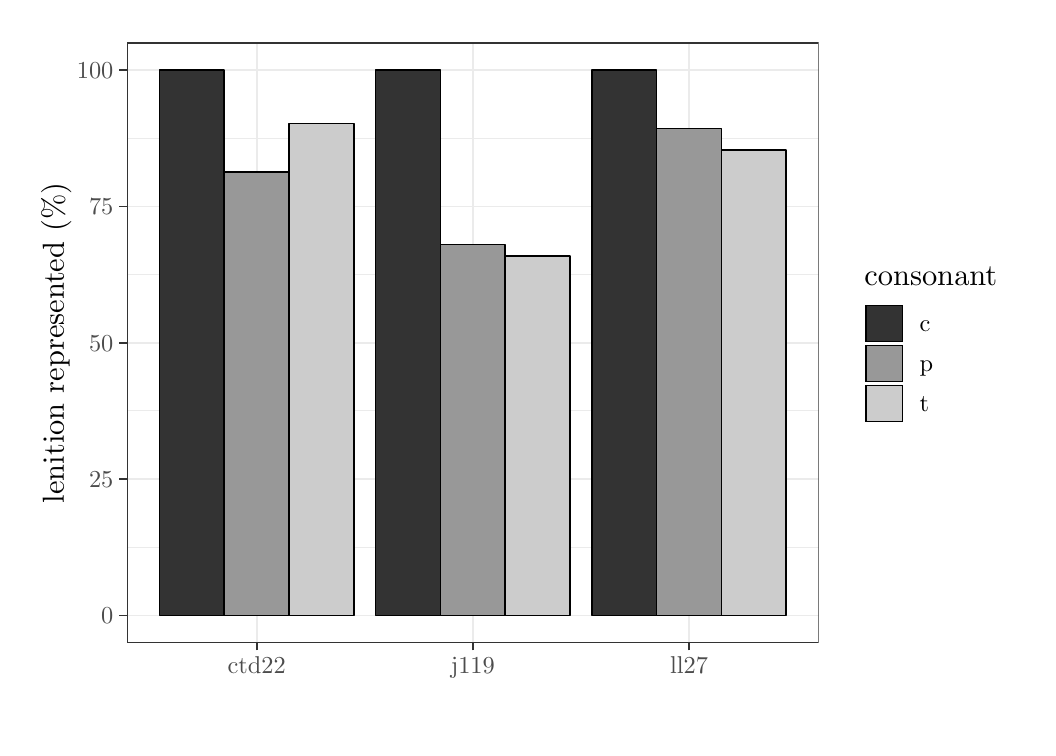
\begin{tikzpicture}[x=1pt,y=1pt]
\definecolor{fillColor}{RGB}{255,255,255}
\path[use as bounding box,fill=fillColor,fill opacity=0.00] (0,0) rectangle (361.35,252.94);
\begin{scope}
\path[clip] (  0.00,  0.00) rectangle (361.35,252.94);
\definecolor{drawColor}{RGB}{255,255,255}
\definecolor{fillColor}{RGB}{255,255,255}

\path[draw=drawColor,line width= 0.6pt,line join=round,line cap=round,fill=fillColor] (  0.00,  0.00) rectangle (361.35,252.94);
\end{scope}
\begin{scope}
\path[clip] ( 35.92, 30.72) rectangle (285.83,247.45);
\definecolor{fillColor}{RGB}{255,255,255}

\path[fill=fillColor] ( 35.92, 30.72) rectangle (285.83,247.45);
\definecolor{drawColor}{gray}{0.92}

\path[draw=drawColor,line width= 0.3pt,line join=round] ( 35.92, 65.20) --
	(285.83, 65.20);

\path[draw=drawColor,line width= 0.3pt,line join=round] ( 35.92,114.46) --
	(285.83,114.46);

\path[draw=drawColor,line width= 0.3pt,line join=round] ( 35.92,163.71) --
	(285.83,163.71);

\path[draw=drawColor,line width= 0.3pt,line join=round] ( 35.92,212.97) --
	(285.83,212.97);

\path[draw=drawColor,line width= 0.6pt,line join=round] ( 35.92, 40.58) --
	(285.83, 40.58);

\path[draw=drawColor,line width= 0.6pt,line join=round] ( 35.92, 89.83) --
	(285.83, 89.83);

\path[draw=drawColor,line width= 0.6pt,line join=round] ( 35.92,139.08) --
	(285.83,139.08);

\path[draw=drawColor,line width= 0.6pt,line join=round] ( 35.92,188.34) --
	(285.83,188.34);

\path[draw=drawColor,line width= 0.6pt,line join=round] ( 35.92,237.59) --
	(285.83,237.59);

\path[draw=drawColor,line width= 0.6pt,line join=round] ( 82.78, 30.72) --
	( 82.78,247.45);

\path[draw=drawColor,line width= 0.6pt,line join=round] (160.87, 30.72) --
	(160.87,247.45);

\path[draw=drawColor,line width= 0.6pt,line join=round] (238.97, 30.72) --
	(238.97,247.45);
\definecolor{drawColor}{RGB}{0,0,0}
\definecolor{fillColor}{gray}{0.80}

\path[draw=drawColor,line width= 0.6pt,line join=round,fill=fillColor] ( 94.49, 40.58) rectangle (117.92,218.29);
\definecolor{fillColor}{RGB}{152,152,152}

\path[draw=drawColor,line width= 0.6pt,line join=round,fill=fillColor] ( 71.06, 40.58) rectangle ( 94.49,200.75);
\definecolor{fillColor}{gray}{0.20}

\path[draw=drawColor,line width= 0.6pt,line join=round,fill=fillColor] ( 47.63, 40.58) rectangle ( 71.06,237.59);
\definecolor{fillColor}{gray}{0.80}

\path[draw=drawColor,line width= 0.6pt,line join=round,fill=fillColor] (172.59, 40.58) rectangle (196.02,170.41);
\definecolor{fillColor}{RGB}{152,152,152}

\path[draw=drawColor,line width= 0.6pt,line join=round,fill=fillColor] (149.16, 40.58) rectangle (172.59,174.55);
\definecolor{fillColor}{gray}{0.20}

\path[draw=drawColor,line width= 0.6pt,line join=round,fill=fillColor] (125.73, 40.58) rectangle (149.16,237.59);
\definecolor{fillColor}{gray}{0.80}

\path[draw=drawColor,line width= 0.6pt,line join=round,fill=fillColor] (250.68, 40.58) rectangle (274.11,208.83);
\definecolor{fillColor}{RGB}{152,152,152}

\path[draw=drawColor,line width= 0.6pt,line join=round,fill=fillColor] (227.26, 40.58) rectangle (250.68,216.51);
\definecolor{fillColor}{gray}{0.20}

\path[draw=drawColor,line width= 0.6pt,line join=round,fill=fillColor] (203.83, 40.58) rectangle (227.26,237.59);
\definecolor{drawColor}{gray}{0.20}

\path[draw=drawColor,line width= 0.6pt,line join=round,line cap=round] ( 35.92, 30.72) rectangle (285.83,247.45);
\end{scope}
\begin{scope}
\path[clip] (  0.00,  0.00) rectangle (361.35,252.94);
\definecolor{drawColor}{gray}{0.30}

\node[text=drawColor,anchor=base east,inner sep=0pt, outer sep=0pt, scale=  0.88] at ( 30.97, 37.55) {0};

\node[text=drawColor,anchor=base east,inner sep=0pt, outer sep=0pt, scale=  0.88] at ( 30.97, 86.80) {25};

\node[text=drawColor,anchor=base east,inner sep=0pt, outer sep=0pt, scale=  0.88] at ( 30.97,136.05) {50};

\node[text=drawColor,anchor=base east,inner sep=0pt, outer sep=0pt, scale=  0.88] at ( 30.97,185.31) {75};

\node[text=drawColor,anchor=base east,inner sep=0pt, outer sep=0pt, scale=  0.88] at ( 30.97,234.56) {100};
\end{scope}
\begin{scope}
\path[clip] (  0.00,  0.00) rectangle (361.35,252.94);
\definecolor{drawColor}{gray}{0.20}

\path[draw=drawColor,line width= 0.6pt,line join=round] ( 33.17, 40.58) --
	( 35.92, 40.58);

\path[draw=drawColor,line width= 0.6pt,line join=round] ( 33.17, 89.83) --
	( 35.92, 89.83);

\path[draw=drawColor,line width= 0.6pt,line join=round] ( 33.17,139.08) --
	( 35.92,139.08);

\path[draw=drawColor,line width= 0.6pt,line join=round] ( 33.17,188.34) --
	( 35.92,188.34);

\path[draw=drawColor,line width= 0.6pt,line join=round] ( 33.17,237.59) --
	( 35.92,237.59);
\end{scope}
\begin{scope}
\path[clip] (  0.00,  0.00) rectangle (361.35,252.94);
\definecolor{drawColor}{gray}{0.20}

\path[draw=drawColor,line width= 0.6pt,line join=round] ( 82.78, 27.97) --
	( 82.78, 30.72);

\path[draw=drawColor,line width= 0.6pt,line join=round] (160.87, 27.97) --
	(160.87, 30.72);

\path[draw=drawColor,line width= 0.6pt,line join=round] (238.97, 27.97) --
	(238.97, 30.72);
\end{scope}
\begin{scope}
\path[clip] (  0.00,  0.00) rectangle (361.35,252.94);
\definecolor{drawColor}{gray}{0.30}

\node[text=drawColor,anchor=base,inner sep=0pt, outer sep=0pt, scale=  0.88] at ( 82.78, 19.71) {\gls{ctd22}};

\node[text=drawColor,anchor=base,inner sep=0pt, outer sep=0pt, scale=  0.88] at (160.87, 19.71) {\gls{j119}};

\node[text=drawColor,anchor=base,inner sep=0pt, outer sep=0pt, scale=  0.88] at (238.97, 19.71) {\gls{ll27}};
\end{scope}
\begin{scope}
\path[clip] (  0.00,  0.00) rectangle (361.35,252.94);
\definecolor{drawColor}{RGB}{0,0,0}

\node[text=drawColor,rotate= 90.00,anchor=base,inner sep=0pt, outer sep=0pt, scale=  1.10] at ( 13.08,139.08) {lenition represented (\%)};
\end{scope}
\begin{scope}
\path[clip] (  0.00,  0.00) rectangle (361.35,252.94);
\definecolor{fillColor}{RGB}{255,255,255}

\path[fill=fillColor] (296.83,104.39) rectangle (355.85,173.78);
\end{scope}
\begin{scope}
\path[clip] (  0.00,  0.00) rectangle (361.35,252.94);
\definecolor{drawColor}{RGB}{0,0,0}

\node[text=drawColor,anchor=base west,inner sep=0pt, outer sep=0pt, scale=  1.10] at (302.33,159.73) {consonant};
\end{scope}
\begin{scope}
\path[clip] (  0.00,  0.00) rectangle (361.35,252.94);
\definecolor{fillColor}{RGB}{255,255,255}

\path[fill=fillColor] (302.33,138.80) rectangle (316.78,153.26);
\end{scope}
\begin{scope}
\path[clip] (  0.00,  0.00) rectangle (361.35,252.94);
\definecolor{drawColor}{RGB}{0,0,0}
\definecolor{fillColor}{gray}{0.20}

\path[draw=drawColor,line width= 0.6pt,line cap=round,fill=fillColor] (303.04,139.51) rectangle (316.07,152.54);
\end{scope}
\begin{scope}
\path[clip] (  0.00,  0.00) rectangle (361.35,252.94);
\definecolor{fillColor}{RGB}{255,255,255}

\path[fill=fillColor] (302.33,124.35) rectangle (316.78,138.80);
\end{scope}
\begin{scope}
\path[clip] (  0.00,  0.00) rectangle (361.35,252.94);
\definecolor{drawColor}{RGB}{0,0,0}
\definecolor{fillColor}{RGB}{152,152,152}

\path[draw=drawColor,line width= 0.6pt,line cap=round,fill=fillColor] (303.04,125.06) rectangle (316.07,138.09);
\end{scope}
\begin{scope}
\path[clip] (  0.00,  0.00) rectangle (361.35,252.94);
\definecolor{fillColor}{RGB}{255,255,255}

\path[fill=fillColor] (302.33,109.89) rectangle (316.78,124.35);
\end{scope}
\begin{scope}
\path[clip] (  0.00,  0.00) rectangle (361.35,252.94);
\definecolor{drawColor}{RGB}{0,0,0}
\definecolor{fillColor}{gray}{0.80}

\path[draw=drawColor,line width= 0.6pt,line cap=round,fill=fillColor] (303.04,110.61) rectangle (316.07,123.64);
\end{scope}
\begin{scope}
\path[clip] (  0.00,  0.00) rectangle (361.35,252.94);
\definecolor{drawColor}{RGB}{0,0,0}

\node[text=drawColor,anchor=base west,inner sep=0pt, outer sep=0pt, scale=  0.88] at (322.28,143.00) {\mw{c}};
\end{scope}
\begin{scope}
\path[clip] (  0.00,  0.00) rectangle (361.35,252.94);
\definecolor{drawColor}{RGB}{0,0,0}

\node[text=drawColor,anchor=base west,inner sep=0pt, outer sep=0pt, scale=  0.88] at (322.28,128.54) {\mw{p}};
\end{scope}
\begin{scope}
\path[clip] (  0.00,  0.00) rectangle (361.35,252.94);
\definecolor{drawColor}{RGB}{0,0,0}

\node[text=drawColor,anchor=base west,inner sep=0pt, outer sep=0pt, scale=  0.88] at (322.28,114.09) {\mw{t}};
\end{scope}
\end{tikzpicture}

  \caption{Percentual representation of lenition of voiceless stops in the various recensions of \mw[]{Buchedd Dewi}.}
  \label{fig:barchartdewi}
\end{figure}



The consistency with which lenition of \mw[]{c} is written implies that the Welsh exemplar was written at a time when lenited \mw[]{c} was already written with \mw[]{g}. This pattern of writing lenition of \mw[]{c}, but not \mw[]{p, t} is found from the second half of the thirteenth century onwards. This is evidence that \textcite{Rob_Ystoriaeu11} was right in positing the late thirteenth century as the time when the Welsh translation was composed and \textcite{Eva_Welsh88} was wrong in positing the fourteenth century.

Lenition of the remaining two consonants, \mw[]{p, t}, is written inconsistently. For these consonants, there are two possible scenarios: either lenition is added independently in the three manuscripts, or it is added in a common exemplar and then copied by two or three of these manuscripts. Statistics may help in deciding between these scenarios.

From here on, only lenition of \mw[]{p, t} are discussed, and \mw[]{c} is left out. I do this because \mw[]{c} appears inherited. This leaves 116 data points.

\section{A statistical excursus}
\label{sec:statistical-excursus}


Chapter~\todo{laws}\ref{cha:welsh-laws} shows that texts originally composed in the thirteenth century and then copied in the fourteenth century replace \mw{p, t, c} for lenited voiceless stops with \mw{b, d, g}, but that they never do so completely. Chapter~\todo{brut}\ref{cha:indep-comp-mwbr} shows that original texts composed from the fourteenth century onwards do write lenited voiceless stops with \mw{b, d, g} consistently.

Taking the insights from these two chapters together, we are able to test whether a Welsh text found in the fourteenth century or later has a Welsh-language ancestor from the thirteenth century or earlier. If lenition of voiceless stops is represented haphazardly, this is evidence it dates from before the fourteenth century. Subfigure~\ref{sfig:pre1250} illustrates this scenario. If lenition of voiceless stops is written consistently, then there is no evidence of a pre-fourteenth-century composition. Subfigure~\ref{sfig:post1250} illustrates this scenario.

It is also possible to diagnose whether two exemplars of a text originally composed in the thirteenth century or earlier have a shared common ancestor from after the thirteenth century. Subfigure~\ref{sfig:intermediate} illustrates this scenario. If we hypothesise that two texts have a stemma of the type found in Subfigure~\ref{sfig:intermediate}, we would expect partial orthographic lenition of voiceless stops in both manuscripts, but the specific instances of lenition or lack thereof would agree with each other in more instances than what would be expected from chance.

\begin{figure}[h]
  \centering
  \subfloat[]{
    \label{sfig:pre1250}
    \begin{forest}
      [μ < 1250
      [X > 1300]
      [Y > 1300]]
    \end{forest}}
  \subfloat[]{
    \label{sfig:post1250}
    \begin{forest}
      [μ > 1300
      [X > 1300]
      [Y > 1300]]
    \end{forest}}
    \subfloat[]{
    \label{sfig:intermediate}
    \begin{forest}
      [μ < 1250
      [ν > 1300
      [X > 1300]
      [Y > 1300]]]
    \end{forest}}
  \caption{Hypothetically reconstructable stemmata based on the orthography of lenited voiceless stops.}
  \label{fig:possiblestemmata}
\end{figure}

The scenario of Subfigure~\ref{sfig:post1250} is easy to differentiate from the scenarios of Subfigure~\ref{sfig:pre1250} and Subfigure~\ref{sfig:intermediate}: the only thing one would have to check is whether lenition of voiceless stops is represented consistently. It is harder to differentiate between the remaining two scenarios. In the scenario of Subfigure~\ref{sfig:pre1250}, haphazard lenition would be found in both surviving manuscripts, but lenition or lack thereof would not correspond to one another to a degree beyond what would be predicted by chance. In order to argue for the scenario of Subfigure~\ref{sfig:intermediate}, one would have to demonstrate that the orthography of lenited voiceless stops agrees in so many specific instances that the partial addition of orthographically lenited voiceless stops is unlikely to be due to chance.

We can only say that a pattern is unlikely to be due to chance if we actually know what chance looks like. It is therefore necessary to form a picture of what chance would look like. The expected percentage of instances agreeing between manuscripts X and Y would be calculated as follows:
\[P(\text{X} = \text{Y}) = (P(\text{len.X}) \times P(\text{len.Y})) + (P(\text{len.X}^C) \times P(\text{len.Y}^C))\]
Here, \(P\) stands for the probability of the event in brackets following it, so \(P(\text{X}=\text{Y})\) stands for the probability of manuscript X and Y agreeing, \(P(\text{len.X})\) stands for the rate by which lenition is added in manuscript X, and \(P(\text{len.Y})\) means the same thing for manuscript Y. The \(^C\) stands for the complement of an event, \ie the event not happening. So, the equation above may be phrased as: the probability of X and Y independently agreeing on orthographical lenition is equal to the product of their respective probabilities of adding lenition plus the product of their respective probabilities of not adding lenition.

To make this formula more concrete, let's assume manuscript X adds orthographical lenition in 60\% of its instances, and manuscript Y adds orthographical lenition in 30\% of its instances. X and Y do not share a common ancestor that postdates orthographical lenition. In this case, the expected probability of X and Y agreeing on the orthography of lenition in a specific instance would be:

\[(0.6 \times 0.3) + (0.4 \times 0.7) = 0.18 + 0.28 = 0.46\]

So, any instance of a lenited voiceless stop would have an 18\% probability of being orthographically represented in both manuscripts by coincidence, and would have a 28\% probability of not being represented in both manuscripts. They would thus have a probability of 46\% of agreeing. A corpus of 100 instances of lenition of voiceless stops would be expected find 46 in agreement, and 54 in disagreement.

What kind of patterns should we ascribe to common inheritance of orthographical lenition? First of all, chance can be the cause of every single pattern, so one cannot completely exclude coincidence as the cause for a group of extremely similar looking manuscripts. We can merely reject chance as a factor because it is \emph{unlikely} to have been the cause of a particular pattern, not because it is \emph{impossible}.

Sciences employing quantitative methods typically reject the null hypothesis if a correlation at least as strong as the observed results has a lower than one in twenty probability of being observed due to chance.  The null hypothesis is the hypothesis that there is no relationship between two measured phenomena. In this case, it would be the hypothesis that the orthography of lenition in manuscript X is unrelated to that in manuscript Y, \ie lenition is added independently in two manuscripts. The opposite of the null hypothesis is the alternative hypothesis, which is the hypothesis that two measured phenomena are related. In this case, this would mean that the orthography of lenition in two mansucripts is related through a common ancestor.

% \subsection{Simulating the null hypothesis in R}
% \label{sec:simul-null-hypoth}

In order to find out whether the occurrences of lenition of \mw[]{p, t} in \gls{j119}, \gls{ll27}, and \gls{ctd22} occur independently of one another, one would have to simulate a scenario where lenition occurs to the same degree as is found in two of our manuscripts, but is distributed randomly. Then, one could compare how lenition and non-lenition is expected to be shared between two manuscripts against their observed counterparts. These results may  be compared to the observed results in order to see how far removed the observed results are from the expected results.

\section{Pearson's chi-squared test }
\label{sec:pearsons-chi-squared}


A statistical test called Pearson's chi-squared test (\(\chi^2\)) of independence may be applied to compare a set of observed values with its expected counterparts. This test allows one to assess whether the  observations on two or more variables are independent of each other.

It assesses the independence of two variables by calculating their expected values and then measures the difference between these values and their observed counterparts. These measurements generate a \(\chi^2\)-score which may in turn be used to calculate the probability of the null hypothesis being true \ie the probability of  representation of lenition in one manuscript and representation of lenition in another being independent variables. When this probability that the observations are independent is lower than five per cent (\emph{p} < 0.05), a correlation is usually held to exist.

In order to perform this test, one first needs to create a contingency table for the observed values, where the different rows represent one variable, and columns represent another variable. Each row in this table represents one variant of the row variable, and each column represents one variant of the column variable~\autocite[754]{MS_Statistics09}.

For example, when comparing how lenition is represented in manuscripts X and Y, manuscript X could be the row variable and Y the column variable. This table would then consist of two rows: one containing instances where lenition is not represented in X, \ie archaisms (A), and one for instances where it is represented, \ie innovations (I).  It would also consist of two columns: one containing the archaisms in Y, and another containing the innovations in Y. The top left cell in this \(2 \times 2\) table would contain the number of instances that are archaisms in both manuscripts (AA), the bottom left cell would contain the amount of archaisms in manuscript X that are innovations in manuscript Y (AI), the top right cell would contain the number innovations in manuscript X and archaisms in manuscript Y (IA), and the bottom right cell would contain the number of shared innovations (II). Table~\ref{tab:obsll27ctd22} is an example of such a contingency table for observed values.

The next step is to calculate the expected values from these observed values. Expected values may be calculated for each cell in row \(i\) and column \(j\) in a contingency table using the following formula:
\[E_{ij}=\frac{(R_i)(C_j)}{n}\]
where \(R_i\) stands for the total of row \(i\), \(C_j\) for the total of column \(j\), and \(n\) for the sample size~\autocite[755--756]{MS_Statistics09}. Table~\ref{tab:expll27ctd22} is an example of a table containing expected cell counts.



Now, the \(\chi^2\) test allows us to test whether the rows and columns are associated to a statistically significant degree, \ie whether there is a dependence between the orthography of lenition in manuscript X and Y. The \(\chi^2\) statistic is the sum of the squared residual values:
\[\chi^2=\sum{\frac{(O-E)^2}{E}}\]
Here, \(O\) stands for the observed values, \eg the values given in Table~\ref{tab:obsll27ctd22}, and \(E\) stands for expected values, \eg the value given in Table~\ref{tab:expll27ctd22}. A large value for \(\chi^2\) implies that the observed counts are not close to their expected counterparts, and therefore that the null hypothesis of independence is false~\autocite[756--757]{MS_Statistics09}. The higher the \(\chi^2\) statistic, the lower the probability that the variables are independent, \eg that representation of lenition in manuscript X is independent from that of manuscript Y. When dealing with a \(2 \times 2\) contingency table, the minimal value for the \(\chi^2\) statistic required to reject the null hypothesis at \textit{p} < 0.05 is 3.841~\autocite[798]{MS_Statistics09}.

If we find that a dependence between the two variables indeed exists, it may be worthwhile to individually calculate the squared residuals that, when summed, form the \(\chi^2\) statistic. This may be done as follows:
\[\frac{(O-E)^2}{E}\]
Doing so allows one to quantify how much each cell value contributes to the significance of the result. This, in turn, may help in deciding which individual instances are worth taking a closer look at. An example of these individual squared residuals is given in Table~\ref{tab:contrll27ctd22}.

% This is exactly what I have done using a programming language for statistical computing called R. I have written a function\todo{I should include the code for this function in an appendix} that takes the following values as its input:
% \begin{itemize}
% \item Corpus size, \ie the amount of data points to be simulated for
%   each manuscript;
% \item Amount of instances of lenition in MS 1;
% \item Amount of instances of lenition in MS 2;
% \end{itemize}
% As its output, it returns four numbers:
% \begin{itemize}
% \item AA, \ie the amount of shared archaisms between MS 1 \& 2;
% \item AI, \ie the amount of archaisms in MS 1 that are innovations in MS 2;
% \item IA, \ie the amount of innovations in MS 1 that are archaisms in MS 2;
% \item II, \ie the amount of shared innovations between MS 1 \& 2.
% \end{itemize}

% Running this function once creates a single set of four numbers showing one instance of the values randomly distributed lenition could generate. Running this function many times over with the same input allows one to calculate the mean value for each of these numbers. It also generates a distribution of these values. Such a distribution of values arising from a simulation makes it possible to calculate the percentile observed values fall in.

% A percentile is a measure indicating the value below which a given percentage of observations fall. So if we simulate a 100 values, and 80 per cent of these simulated values are lower than or equal to the observed value, then we can say that the observed value falls in the 80\textsuperscript{th} percentile.

% If an observed value falls within the 95\textsuperscript{th} percentile of all simulated values, then we can say that the probability that the simulation would return a value at least as high is lower than five per cent. In other words, the probability of the observed value being at least as high as it is would be lower than five per cent. If this is the case, the observed value may be said to be statistically significant.

The \(\chi^2\) test can be unreliable when the absolute amount of expected values is too low. In a two-by-two contingency table such as the ones discussed here, each expected cell count should be at least 5. This condition is in fact not always met using the data from \mw[]{Buchedd Dewi}. In such a case, Yates' correction for continuity may be applied to the \(\chi^2\) test by subtracting 0.5 from the difference between every observed value and its expected counterpart:

\[\chi_\text{Yates}^2 =  \frac{(|O - E| - 0.5)^2}{E}\]

A test using this correction is more conservative than one not using it, \ie it produces lower \(\chi^2\) statistics and therefore gives more results that fail to reject the null hypothesis. For contingency tables given in this chapter, I have found that applying this correction never gives cause to reject the null hypothesis.\todo{find authoritative source to back me up on this continuity correction}


\subsection{The chi-square tests applied}
\label{sec:chisqapplied}

The observed values for the relationship between \gls{ll27} and \gls{ctd22} are found in Table~\ref{tab:obsll27ctd22}. 

\begin{table}[h]
  \centering
  \begin{tabular}{ccddd}
\toprule
 & & \tchhh{\gls{ll27}} \\
& & \tch{A} & \tch{I} & \tch{Total}\\
\multirow{3}{*}{\gls{ctd22}} & A  & 6 & 12 & 18\\
& I & 8 & 90 & 98\\
& Total & 14 & 102 & 116\\\bottomrule
\end{tabular}
  \caption{Observed values for the relationship between \gls{ll27} and \gls{ctd22}}
  \label{tab:obsll27ctd22}
\end{table}

% The corpus size is 117. Lenition of \mw[]{p, t} is represented in 103 instances in \gls{ll27}, and in 98 instances in \gls{ctd22}. The expected amount of shared innovations is calculated by multiplying the product of the respective rates of lenition by the corpus size (\(N\)):

% \[P(\text{rep.\gls{ll27}}) \times P(\text{rep.\gls{ctd22}}) \times N = \frac{103}{117} \times \frac{98}{117} \times 117 \approx 86 \]

% So we would expect 86 forms to be lenited in both \gls{ll27} and \gls{ctd22}, compared to the observed 90 forms. The expected amount of shared archaisms is similarly calculated, only the complement of the rate of lenitionis used, \ie the rate of non-lenition:

% \[P(\text{rep.\gls{ll27}}^C) \times P(\text{rep.\gls{ctd22}}^C) \times N = \frac{117-103}{117} \times \frac{117-98}{117} \times 117 \approx 2 \]

% So we would expect about 2 forms to be lenited in both texts, compared to the observed 6 forms. Both the observed shared archaisms (AA) and the observed shared innovations (II) are more numerous than their expected counterparts. This gives credence to the idea that the specific instances of lenition of \mw[]{p, t} in \gls{ll27} and \gls{ctd22} are inherited through a common ancestor.

The expected values for Table~\ref{tab:obsll27ctd22} are given in Table~\ref{tab:expll27ctd22}. As can be seen, they sometimes differ quite a bit from their observed counterparts. Especially the observed number of shared archaisms far exceeds its expected counterpart. 

\begin{table}[h]
  \centering
  \begin{tabular}{ccddd}
\toprule
 & & \tchhh{\gls{ll27}} \\
& & \tch{A} & \tch{I} & \tch{Total}\\
\multirow{3}{*}{\gls{ctd22}} & A  & 2.17 & 15.83 & 18\\
& I & 11.83 & 86.17 & 98\\
& Total & 14 & 102 & 116\\\bottomrule
\end{tabular}
  \caption{Expected values for the relationship between \gls{ll27} and \gls{ctd22}}
  \label{tab:expll27ctd22}
\end{table}

% Using my own function in R, I performed 1000 simulations of two manuscripts with 117 data points, with the first manuscript having 103 instances of lenition, and the second having 98, just like \gls{ll27} and \gls{ctd22}. The function then counted how many data points fell in each of the four categories (AA, AI, IA, II). The observed numbers of agreement compared to these simulations  corresponded to the percentiles given in Table~\ref{tab:percentilesll27ctd22}.

% \begin{table}[htbp]
%   \centering
%   \begin{tabular}{ccdd}
%     \toprule
%        &    & \tchh{\gls{ll27}}   \\
%        &    & \tch{A}  & \tch{I} \\
%     \multirow{2}{*}{\gls{ctd22}} & A  & 99.8 & 0.0 \\
%        & I  & 93.5 & 99.8 \\\bottomrule
%     \end{tabular}%
%     \caption{Percentiles }
%     \label{tab:percentilesll27ctd22}%
% \end{table}%

% Table~\ref{tab:percentilesll27ctd22} must be read as follows: the percentile 99.8 means that 99.8\% of simulations yielded a value equal to or lower than the observed value, and 0.2\% yielded a higher value. Therefore, any result corresponding to a percentile greater than 95 or lesser than 5 is significant, because the probability of such a result is lower than 5\%.

A \(\chi^2\) test performed on the correspondences between these two manuscripts yields the following result: \(\chi^2\) = 9.08, yielding the probability \emph{p} < 0.005 at one degree of freedom, so the correlation between the orthography of lenition in \gls{ll27} and \gls{ctd22} is  significant at \textit{p} < .05.

Because a dependence between the two variables is established, it is fitting to find out what values specifically make for this outcome. More concretely, we want to know to what degree it is either the shared archaisms or the shared innovations that make the relationship between archaisms and innovations in \gls{ll27} and \gls{ctd22} statistically significant. Table~\ref{tab:contrll27ctd22} gives the \(\chi^2\) statistic broken down for the individual cell values.

\begin{table}[h]
  \centering
  \begin{tabular}{ccddd}
\toprule
 & & \tchhh{\gls{ll27}} \\
& & \tch{A} & \tch{I} & \tch{Total}\\
\multirow{3}{*}{\gls{ctd22}} & A  & 6.74 & 0.93 & 7.67\\
& I & 1.24 & 0.17 & 1.41\\
& Total & 7.98 & 1.1 & 9.08\\\bottomrule
\end{tabular}
  \caption{Squared residuals for the relationship between \gls{ll27} and \gls{ctd22}}
  \label{tab:contrll27ctd22}
\end{table}

These calculations tell us the following:
\begin{itemize}
\item The amount of archaisms and innovations shared between \gls{ll27} and \gls{ctd22} is beyond what we may attribute to chance.
\item The amount of shared archaisms between \gls{ll27} and \gls{ctd22} is the furthest removed from what would be expected from chance, compared to shared innovations or archaisms in one manuscript that are innovations in another.
\end{itemize}

Two more pairs of relationships may be analysed: the relationship between \gls{j119} and \gls{ll27}, and the relationship between \gls{j119} and \gls{ctd22}. Table~\ref{tab:continj119ll27} gives the contingency tables for the former relationship, and Table~\ref{tab:continctd22j119} gives the contingency tables for the latter relationship. For both of these pairings, the \(\chi^2\) statistic, \ie the sum of the squared residuals, exceeds the \(\chi^2\) statistic of \gls{ll27} and \gls{ctd22}. All three pairings show a statistically significant relationship at \textit{p} < .05. The squared residuals are again the highest for the shared archaisms in both cases, so it is the archaisms shared between any pair that merit further research. The next section will focus on these archaisms

\begin{table}[h]
  \centering
  \subfloat[Observed values.]{%
    \begin{tabular}{ccddd}
\toprule
 & & \tchhh{\gls{j119}} \\
& & \tch{A} & \tch{I} & \tch{Total}\\
\multirow{3}{*}{\gls{ll27}} & A  & 11 & 3 & 14\\
& I & 27 & 75 & 102\\
& Total & 38 & 78 & 116\\\bottomrule
\end{tabular}%
  }%
  \hfill
  \subfloat[Expected values.]{%
    \begin{tabular}{ccddd}
\toprule
 & & \tchhh{\gls{j119}} \\
& & \tch{A} & \tch{I} & \tch{Total}\\
\multirow{3}{*}{\gls{ll27}} & A  & 4.59 & 9.41 & 14\\
& I & 33.41 & 68.59 & 102\\
& Total & 38 & 78 & 116\\\bottomrule
\end{tabular}%
  }
  
  \subfloat[Squared residuals.]{%
    \begin{tabular}{ccddd}
\toprule
 & & \tchhh{\gls{j119}} \\
& & \tch{A} & \tch{I} & \tch{Total}\\
\multirow{3}{*}{\gls{ll27}} & A  & 8.97 & 4.37 & 13.34\\
& I & 1.23 & 0.6 & 1.83\\
& Total & 10.2 & 4.97 & 15.17\\\bottomrule
\end{tabular}%
  }
  \caption{Contingency tables for the relationship between \gls{j119} and \gls{ll27}.}
  \label{tab:continj119ll27}
\end{table}

\begin{table}[h]
  \centering
  \subfloat[Observed values.]{%
    \begin{tabular}{ccddd}
\toprule
 & & \tchhh{\gls{ctd22}} \\
& & \tch{A} & \tch{I} & \tch{Total}\\
\multirow{3}{*}{\gls{j119}} & A  & 13 & 25 & 38\\
& I & 5 & 73 & 78\\
& Total & 18 & 98 & 116\\\bottomrule
\end{tabular}%
  }%
  \hfill
  \subfloat[Expected values.]{%
    \begin{tabular}{ccddd}
\toprule
 & & \tchhh{\gls{ctd22}} \\
& & \tch{A} & \tch{I} & \tch{Total}\\
\multirow{3}{*}{\gls{j119}} & A  & 5.9 & 32.1 & 38\\
& I & 12.1 & 65.9 & 78\\
& Total & 18 & 98 & 116\\\bottomrule
\end{tabular}%
  }

  \subfloat[Squared residuals.]{%
    \begin{tabular}{ccddd}
\toprule
 & & \tchhh{\gls{ctd22}} \\
& & \tch{A} & \tch{I} & \tch{Total}\\
\multirow{3}{*}{\gls{j119}} & A  & 8.56 & 1.57 & 10.13\\
& I & 4.17 & 0.77 & 4.93\\
& Total & 12.73 & 2.34 & 15.06\\\bottomrule
\end{tabular}%
  }
  \caption{Contingency tables for the relationship between \gls{j119} and \gls{ctd22}.}
  \label{tab:continctd22j119}
\end{table}


\section{The evidentiary value of these tests}
\label{sec:evidence-from-these}



The p-value is well below .05 for all three combinations of manuscripts. The most obvious interpretation of these observations would be that lenition of \mw[]{p, t} was added to an exemplar common to all three manuscripts. This means we may reconstruct the stemma found in Figure~\ref{fig:stemmachisquare} based purely on \(\chi^2\)-tests.

\begin{figure}[h]
  \centering
  \begin{forest}
    where n children=0{tier=word}{}
    [α
    [\textit{β}
    [\gls{j119}]
    [\gls{ll27}]
    [\gls{ctd22}]
    ]{\draw[<-]()--++(1.5cm,0cm) node[anchor=west]{lenited \mw{p, t} partially represented};}
    ]{\draw[<-]()--++(1.5cm,0cm) node[anchor=west]{lenited \mw{c} fully represented};}
  \end{forest}
  \caption{Stemma of  \mw[]{Buchedd Dewi} as far as the \(\chi^2\)-tests are concerned.}
  \label{fig:stemmachisquare}
\end{figure}

We were able to confirm the date of the original Welsh translation (manuscript α) to the second half of the thirteenth century based on its representation of lenited \mw{c} alone. We may similarly date manuscript \textit{β} to around 1300 or later, because this is when lenition of \mw{p, t} was written. Note that \textcite[liv]{Eva_Welsh88} posited the fourteenth century as the period in which the Welsh translation (\textit{α}) was produced. I hold this to be unlikely due to the complete representation of lenited \mw[]{c}, but partial representation of lenited \mw[]{p, t}. However, it does seem that the last common ancestor of the extant texts (\textit{β}) dates from the fourteenth century. 

A comparison of Figure~\ref{fig:stemmachisquare}. with Figure~\ref{fig:stemmadewievans} on page \pageref{fig:stemmadewievans} shows that the \(\chi^2\)-tests are able to confirm the existence of hypothetical manuscript \textit{β}, but they do not provide evidence for any further division between the manuscripts. We are unable to establish the existence or the position of a manuscript \textit{γ} hypothesised by Evans based on these tests.

The statistics demonstrate that there is a correlation between whether an instance of \mw{p, t} is lenited in two manuscripts, and this correlation is found for every single pairing of manuscripts. This is evidence for a common core of lenited \mw[]{p, t} inherited from a single manuscript, although more instances were added to each manuscript independently. 

However, there still remains the possibility that the orthography of lenition correlates in two manuscripts for other reasons than common inheritance. The tests conducted  only confirm that the variable of representation of lenition in one manuscript is dependent on this  variable in another manuscript. Strictly speaking, they do not necessarily confirm that this dependency of representation of lenition is inherited from a common exemplar.

Alternatively, the dependency could have arisen because the various scribes modernised their texts under the same general principles, \eg if two scribes added lenition independently, but both scribes added lenition following \mw[your]{dy}, but not following \mw[on]{ar}, then the dependency of representation of lenition in their respective manuscripts would turn out to be significant, but this would not be due to common inheritance. The implications of this possibility, and how to exclude this possibility are discussed in Section~\ref{sec:shar-innov-arch}. 


\section{The shared archaisms}
\label{sec:beyond-stat-again}

Both the issue of further subgrouping the three manuscripts and the  possibility that the dependency of representation is not due to common inheritance require further investigation. The results may help us in deciding where in particular to look. We saw that the largest contributions made to the \(\chi^2\)-statistic came from the shared archaisms, so the observed amounts of shared archaisms depart the most from their expected counterparts. This begs the question what these examples are, and what they have in common. 

% Let's take a closer look at one example, the instance of \mw[as {[}the{]} kingdom]{yn teyrnas}:

% \begin{mwl}
%   \mwc[ex:ynteyrnasj119]{\gls{j119} 99r.17--21}{a mi heb ef a ỽeleis angel yn dyuot attaỽ ac yn galỽ arnaỽ ac yn erchi idaỽ vynet y ỽlat y gyuanhedu y lle a barchassei duỽ idaỽ yn teyrnnas demetica. Sef yỽ honno mynyỽ yn y deheu.}{``And I,'' said he, ``saw an angel coming towards him and calling to him and requesting him to go to the country to settle the place that God kept apart for him in/as the kingdom of Dyfed. This is that kingdom: Mynyw in the south.''}
%   \mwc[ex:ynteyrnasll27]{\gls{ll27} 67v.20--23}{a mi a weleis heb ef angel yn dyuot attaỽ ac yn galỽ arnaỽ. ac yn erchi idaỽ vynet y wlat y gyfanhedu y ỻe a barchassei duỽ idaỽ yn teyrnas demetica. Sef yỽ honno mynyỽ yn y deheu.}{``And I saw,'' said he, ``an angel coming towards him and calling to him and requesting him to go to the country to settle in the place that God kept apart for him in/as the kingdom of Dyfed. This is that kingdom: Mynyw in the south.''}
%   \mwc[ex:ynteyrnasctd22]{\gls{ctd22} 148r.3--7}{a mi a weleis heb ef agel yn dyuot attaỽ ac yn galỽ arnaỽ ac yn erchi idaỽ vynet y wlat y gyuanhedu y lle a barthassei duỽ ydaỽ y teyrnas demetica. sef yỽ honno mynyỽ yn y deheu.}{``And I saw,'' said he, ``an angel coming towards him and calling to him and requesting him to go to the country to settle in the place that God kept apart for him in/as the kingdom of Dyfed. This is that kingdom: Mynyw in the south.''}
% \end{mwl}

% In \gls{mow}, the verb \mow[divide]{parthu} goes with the \mow[into]{yn} which causes lenition, as can be seen from some of their examples in~\textcite[s.v.~\textit{parthaf; parthu}]{bevan_geiriadur_2014}:  `\mow{parthodd ef J bobyl yn dair byddin}. [\dots] \mow{wrth barthu‘r gramar, yn bedair colofn}'. The verb \mow[]{parchu} in the meaning of `keep apart, ordain' is somewhat rare and does not have any examples followed by \mow[]{yn} save for the one in \mw[]{Buchedd Dewi} discussed here. Under this analysis orthographic lenition is indeed expected but lacking in \mw[]{teyrnas}. On the other hand, the next sentence identifies not Dyfed, but Mynyw as the area kept apart. Mynyw lies in Dyfed, so \mw[]{yn} should be analysed as the \mw[]{yn} causing nasalisation rather than lenition, disqualifying this instance as a shared lack of orthographical lenition, as there is no lenition in the first place. In this case, a better translation would perhaps be `the place that God kept apart for him in the kingdom of Dyfed, namely Mynyw in the south'.

\begin{mwl}
  \mwc[ex:hyttrannoethj119]{\gls{j119} 96v.9--10}{Ac yna deỽi ae disgyblon a dyrỽwestassant y nos honno hyt \al{trannoeth}.}{And then David and his disciples fasted that night until the next day.}
  \mwc[ex:hyttrannoethll27]{\gls{ll27} 65v.15--16}{Ac yna dewi ae disgyblon a dyrwestassant y nos honno hyt \al{trannoeth}.}{And then David and his disciples fasted that night until the next day.}
  \mwc[ex:hyttrannoethctd22]{\gls{ctd22} 143v.6--8}{ac yna dewi ae disgyblon a dyrwestassant y nos honno hyt \al{trannoeth}.}{And then David and his disciples fasted that night until the next day.}
\end{mwl}

It is beyond doubt that \mw[until]{hyt} causes lenition, but this instance contains the \gls{doubconclus} \mw{-t t-}. Because of this environment, non-representation of lenition could be argued to be trivial, because there is no phonological lenition to be represented in the first place. On the other hand, it could be argued that the very fact that writing lenition is optional here makes these instances good candidates for analysing the relationship between different manuscript versions.

In the particular case of the example above this point is moot. All three manuscripts lack orthographical lenition, so they cannot be used to triangulate the exact relationship between them. However, the next example supports the argument that non-leniting phonological value do have evidential value in stemmatics, because non-lenition and lenition sometimes stand in opposition in this phonological environment.

\begin{mwl}
  \mwc[ex:ynysprydeinj119]{\gls{j119} 101r.18--19}{Ac vrth hynny y gỽnaethpỽyt deỽi sant yn tyỽyssaỽc ac yn pennadur ar seint ynys \al{prydein}}{And accordingly saint David was made prince and ruler of the saints on the island of Britain.}
  \mwc[ex:ynysprydeinll27]{\gls{ll27} 69r.22--23}{Ac ỽrth hynny y gỽnaethpỽyt dewi sant yn bennadur ac yn tywyssaỽc ar seint ynys \al{prydein}.}{And accordingly saint David was made  ruler and prince of the saints on the island of Britain.}
  \mwc[ex:ynysprydeinctd22]{\gls{ctd22} 151r.11--12}{ac ỽrth hynny y gỽnaethpỽyt dewi sant yn bennadỽr.\ ac yn dywyssaỽc ar seint ynys \al{prydein}.}{And accordingly saint David was made  ruler and prince of the saints on the island of Britain.}
\end{mwl}

Here, the orthographical non-lenition of  consonant cluster \mw{-s \gls{T}-} is also expected from a phonological point of view, because there is no phonetic or phonological difference between voiced and voiceless stops following \mw[]{-s}. However, many other instances of \mw{-s \gls{T}-} do write lenition, \ie \mw[island of Britain]{ynys brydein}. All other instances of \mw[]{ynys brydein} do show lenition in \gls{ctd22}, and so does one instance in \gls{ll27}\footnote{They are found in \gls{ll27} 69.15 and \gls{ctd22} 147r.12, 151r.2, 151r.10, and 151v.2.}. This makes this particular shared archaism non-trivial from an orthographic point of view, so the existence of this variation in orthography implies that non-leniting consonant clusters may be used in establishing the stemmatic relationship between  manuscripts. 


\begin{table}[h]
  \begin{tabular}{wlddcddcddc}
    \toprule
    & & \multicolumn{3}{c}{\gls{j119}} & \multicolumn{3}{c}{\gls{ll27}} & \multicolumn{3}{c}{\gls{ctd22}} \\
    \tch{Word} & \tch{Cause lenition}  & \tch{f.} & \tch{l. } & \tch{len.} & \tch{f.} & \tch{l. } & \tch{len.} & \tch{f.} & \tch{l. } & \tch{len.} \\
    \midrule
    ben & \mw{uch} & 93r & 14 & \TRUE & 63r & 6  & \FALSE & 138r & 14 & \FALSE \\
    Badrig & fem.\ noun & 93v & 8  & \FALSE & 63r & 22 & \TRUE & 138v & 16 & \FALSE \\
    bregethu & obj. & 94r & 13 & \FALSE & 63v & 20 & \TRUE & 139v & 15 & \FALSE \\
    bennaduriaeth & parenthesis & 94r & 22 & \FALSE & 64r & 1  & \TRUE & 140r & 8  & \FALSE \\
    Baulinus & \mw{at} & 95r & 12 & \FALSE & 64v & 7  & \TRUE & 141r & 15 & \FALSE \\
    Bebiog & \mw{y} ‘to' & 95r & 23 & \FALSE & 64v & 16 & \FALSE & 141v & 10 & \TRUE \\
    dan & obj. & 95v & 17 & \FALSE & 65r & 5  & \TRUE & 142r & 12 & \FALSE \\
    dan & obj. & 95v & 16 & \FALSE & 65r & 5  & \TRUE & 142r & 12 & \FALSE \\
    Basg & fem.\ noun & 97r & 25 & \FALSE & 66r & 23 & \TRUE & 145r & 2  & \FALSE \\
    dri & \mw{y} ‘to' & 97v & 4  & \FALSE & 66r & 27 & \FALSE & 145r & 7  & \TRUE \\
    dair & \mw{yn} & 98r & 18 & \FALSE & 67r & 4  & \FALSE & 146r & 14 & \TRUE \\
    Brydain & fem.\ noun & 98v & 21 & \FALSE & 67v & 2  & \FALSE & 147r & 12 & \TRUE \\
    bregethu & obj. & 98v & 22 & \TRUE & 67v & 3  & \FALSE & 147r & 13 & \FALSE \\
    bregethu & parenthesis & 100v & 13 & \FALSE & 68v & 22 & \TRUE & 150r & 10 & \FALSE \\
    dywysog & \mw{yn} & 101r & 9  & \FALSE & 69r & 14 & \FALSE & 151r & 1  & \TRUE \\
    bennadur & obj. & 101r & 11 & \FALSE & 69r & 15 & \TRUE & 151r & 3  & \FALSE \\
    bennadur & obj. & 101r & 12 & \FALSE & 69r & 15 & \TRUE & 151r & 5  & \FALSE \\
    Brydain & fem.\ noun & 101r & 18 & \FALSE & 69r & 21 & \FALSE & 151r & 10 & \TRUE \\
    dywysog & \mw{yn} & 101r & 19 & \FALSE & 69r & 23 & \FALSE & 151r & 12 & \TRUE \\
    bregethu & obj. & 101r & 21 & \TRUE & 69r & 24 & \FALSE & 151r & 14 & \FALSE \\
    Brydain & fem.\ noun & 101r & 24 & \FALSE & 69r & 27 & \FALSE & 151v & 2  & \TRUE \\
    \bottomrule
  \end{tabular}%
  \caption{Instances where exactly one manuscript represents lenition.}
  \label{tab:exact1mslen}
\end{table}
All other shared archaisms are instances where exactly one manuscript has lenition represented. These are the found in Table~\ref{tab:exact1mslen}. Many instances show the consonant cluster \mw[]{-s \gls{T}-} discussed above, including \mw[Easter night]{nos basc} (\gls{ll27}~66r.23). Beyond this, we have some personal names that are lenited irregularly: \mow[]{Badrig, Baulinus} and  \mow{Bebiog}. In \gls{mow}, lenition of personal names is quite rare, and is even rarer for non-Welsh names such as Paulinus~\autocite[702]{thomas_gramadeg_1996}\footnote{In \gls{mw} lenition is still common here, but translations from Latin may differ from original Welsh compositions in this regard. See Chapter~\ref{cha:indep-comp-mwbr}.}. 

The remaining instances of non-representation do not lend themselves to an easy explanation from a \gls{mow} point of view. Words such as leniting \mw[as, into]{yn} and \mw[to]{y} lenite \mw[]{p, t} consistently, and object lenition and parenthesis also trigger lenition consistently. In \gls{mw}, however, we find that the latter two of these examples are applied much less consistently than the former two. Their difference is that when \mw[]{yn, y} cause lenition, this lenition may be classified as contact lenition, while object lenition and lenition due to parenthesis are examples of free lenition. From a diachronic perspective, contact lenition may as a rule be explained as the reflex of a pre-apocope morpheme-final vowel. Synchronically in \gls{mw} and \gls{mow}, this means that contact lenition is triggered when the lenited word follows a morpheme whose property is to cause lenition. Free lenition, by contrast, is triggered under specific syntactic circumstances, and is usually a post-apocope innovation. Free lenition has gradually gained ground over the \gls{mw} period, and a fixed set of rules governing free lenition over the several hundred years of this period cannot be formulated for this whole period. 

As noted, the database contains  116 entries for \mw[]{p, t}. Of these entries, 95 are instances of contact lenition while only 21 are instances of free lenition. When discounting the instances of \mw[]{-s \gls{T}-} and the personal names, Table~\ref{tab:exact1mslen} gives 9 instances of free lenition, and only 5 instances of contact lenition remain. This gives the impression that representation of free lenition is more likely to vary between manuscripts than contact lenition.

\section{Free lenition}
\label{sec:points-where-one}
If it is true that free lenition shows more orthographical variation between manuscripts than contact lenition, then free lenition may hold the key in further reconstructing the stemma of the manuscripts. Figure~\ref{fig:contfreelendewi} shows how many instances of orthographical lenition are represented 0, 1, 2, or 3 times in the three manuscripts, and divides them between contact lenition and free lenition. The zero instances of free lenition not represented in any manuscript are a result of the methodology used in deciding what should go in the database: because free lenition is applied inconsistently in \gls{mw}, I only record representation if at least one manuscript represents it.

\begin{figure}[h]
  \centering
  % Created by tikzDevice version 0.11 on 2018-12-11 10:42:19
% !TEX encoding = UTF-8 Unicode
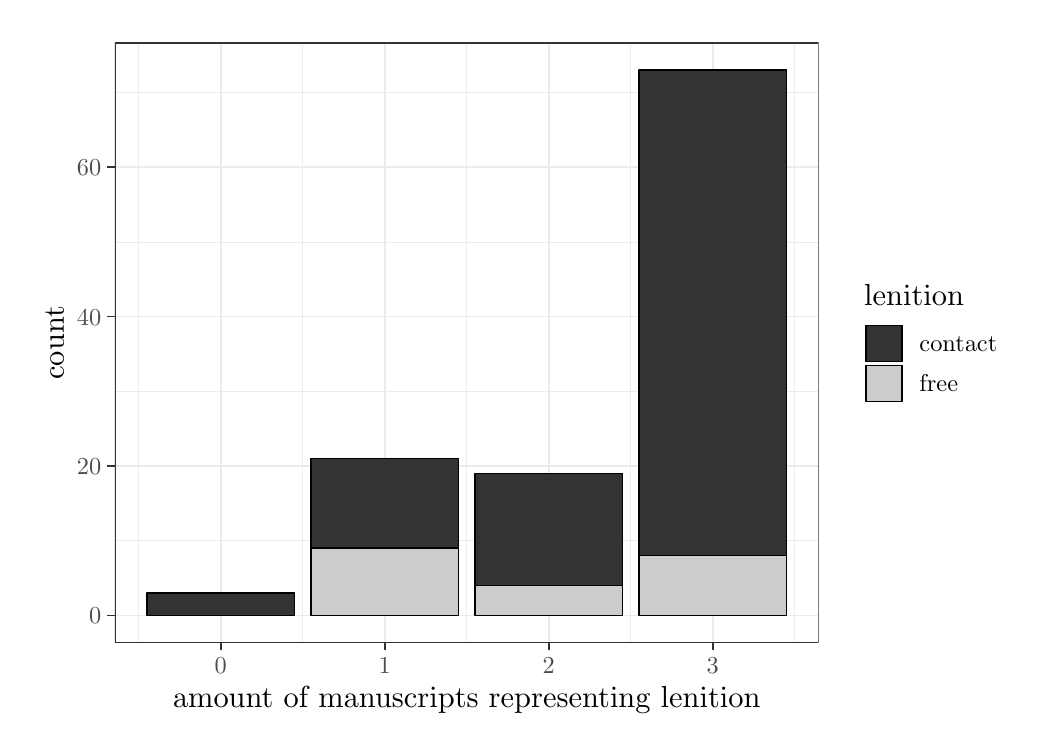
\begin{tikzpicture}[x=1pt,y=1pt]
\definecolor{fillColor}{RGB}{255,255,255}
\path[use as bounding box,fill=fillColor,fill opacity=0.00] (0,0) rectangle (361.35,252.94);
\begin{scope}
\path[clip] (  0.00,  0.00) rectangle (361.35,252.94);
\definecolor{drawColor}{RGB}{255,255,255}
\definecolor{fillColor}{RGB}{255,255,255}

\path[draw=drawColor,line width= 0.6pt,line join=round,line cap=round,fill=fillColor] (  0.00,  0.00) rectangle (361.35,252.94);
\end{scope}
\begin{scope}
\path[clip] ( 31.52, 30.72) rectangle (285.79,247.45);
\definecolor{fillColor}{RGB}{255,255,255}

\path[fill=fillColor] ( 31.52, 30.72) rectangle (285.79,247.45);
\definecolor{drawColor}{gray}{0.92}

\path[draw=drawColor,line width= 0.3pt,line join=round] ( 31.52, 67.56) --
	(285.79, 67.56);

\path[draw=drawColor,line width= 0.3pt,line join=round] ( 31.52,121.54) --
	(285.79,121.54);

\path[draw=drawColor,line width= 0.3pt,line join=round] ( 31.52,175.52) --
	(285.79,175.52);

\path[draw=drawColor,line width= 0.3pt,line join=round] ( 31.52,229.50) --
	(285.79,229.50);

\path[draw=drawColor,line width= 0.3pt,line join=round] ( 40.11, 30.72) --
	( 40.11,247.45);

\path[draw=drawColor,line width= 0.3pt,line join=round] ( 99.38, 30.72) --
	( 99.38,247.45);

\path[draw=drawColor,line width= 0.3pt,line join=round] (158.65, 30.72) --
	(158.65,247.45);

\path[draw=drawColor,line width= 0.3pt,line join=round] (217.93, 30.72) --
	(217.93,247.45);

\path[draw=drawColor,line width= 0.3pt,line join=round] (277.20, 30.72) --
	(277.20,247.45);

\path[draw=drawColor,line width= 0.6pt,line join=round] ( 31.52, 40.58) --
	(285.79, 40.58);

\path[draw=drawColor,line width= 0.6pt,line join=round] ( 31.52, 94.55) --
	(285.79, 94.55);

\path[draw=drawColor,line width= 0.6pt,line join=round] ( 31.52,148.53) --
	(285.79,148.53);

\path[draw=drawColor,line width= 0.6pt,line join=round] ( 31.52,202.51) --
	(285.79,202.51);

\path[draw=drawColor,line width= 0.6pt,line join=round] ( 69.75, 30.72) --
	( 69.75,247.45);

\path[draw=drawColor,line width= 0.6pt,line join=round] (129.02, 30.72) --
	(129.02,247.45);

\path[draw=drawColor,line width= 0.6pt,line join=round] (188.29, 30.72) --
	(188.29,247.45);

\path[draw=drawColor,line width= 0.6pt,line join=round] (247.56, 30.72) --
	(247.56,247.45);
\definecolor{drawColor}{RGB}{0,0,0}
\definecolor{fillColor}{gray}{0.20}

\path[draw=drawColor,line width= 0.6pt,line join=round,fill=fillColor] ( 43.08, 40.58) rectangle ( 96.42, 48.67);
\definecolor{fillColor}{gray}{0.80}

\path[draw=drawColor,line width= 0.6pt,line join=round,fill=fillColor] (102.35, 40.58) rectangle (155.69, 64.87);
\definecolor{fillColor}{gray}{0.20}

\path[draw=drawColor,line width= 0.6pt,line join=round,fill=fillColor] (102.35, 64.87) rectangle (155.69, 97.25);
\definecolor{fillColor}{gray}{0.80}

\path[draw=drawColor,line width= 0.6pt,line join=round,fill=fillColor] (161.62, 40.58) rectangle (214.96, 51.37);
\definecolor{fillColor}{gray}{0.20}

\path[draw=drawColor,line width= 0.6pt,line join=round,fill=fillColor] (161.62, 51.37) rectangle (214.96, 91.85);
\definecolor{fillColor}{gray}{0.80}

\path[draw=drawColor,line width= 0.6pt,line join=round,fill=fillColor] (220.89, 40.58) rectangle (274.23, 62.17);
\definecolor{fillColor}{gray}{0.20}

\path[draw=drawColor,line width= 0.6pt,line join=round,fill=fillColor] (220.89, 62.17) rectangle (274.23,237.59);
\definecolor{drawColor}{gray}{0.20}

\path[draw=drawColor,line width= 0.6pt,line join=round,line cap=round] ( 31.52, 30.72) rectangle (285.79,247.45);
\end{scope}
\begin{scope}
\path[clip] (  0.00,  0.00) rectangle (361.35,252.94);
\definecolor{drawColor}{gray}{0.30}

\node[text=drawColor,anchor=base east,inner sep=0pt, outer sep=0pt, scale=  0.88] at ( 26.57, 37.55) {0};

\node[text=drawColor,anchor=base east,inner sep=0pt, outer sep=0pt, scale=  0.88] at ( 26.57, 91.52) {20};

\node[text=drawColor,anchor=base east,inner sep=0pt, outer sep=0pt, scale=  0.88] at ( 26.57,145.50) {40};

\node[text=drawColor,anchor=base east,inner sep=0pt, outer sep=0pt, scale=  0.88] at ( 26.57,199.48) {60};
\end{scope}
\begin{scope}
\path[clip] (  0.00,  0.00) rectangle (361.35,252.94);
\definecolor{drawColor}{gray}{0.20}

\path[draw=drawColor,line width= 0.6pt,line join=round] ( 28.77, 40.58) --
	( 31.52, 40.58);

\path[draw=drawColor,line width= 0.6pt,line join=round] ( 28.77, 94.55) --
	( 31.52, 94.55);

\path[draw=drawColor,line width= 0.6pt,line join=round] ( 28.77,148.53) --
	( 31.52,148.53);

\path[draw=drawColor,line width= 0.6pt,line join=round] ( 28.77,202.51) --
	( 31.52,202.51);
\end{scope}
\begin{scope}
\path[clip] (  0.00,  0.00) rectangle (361.35,252.94);
\definecolor{drawColor}{gray}{0.20}

\path[draw=drawColor,line width= 0.6pt,line join=round] ( 69.75, 27.97) --
	( 69.75, 30.72);

\path[draw=drawColor,line width= 0.6pt,line join=round] (129.02, 27.97) --
	(129.02, 30.72);

\path[draw=drawColor,line width= 0.6pt,line join=round] (188.29, 27.97) --
	(188.29, 30.72);

\path[draw=drawColor,line width= 0.6pt,line join=round] (247.56, 27.97) --
	(247.56, 30.72);
\end{scope}
\begin{scope}
\path[clip] (  0.00,  0.00) rectangle (361.35,252.94);
\definecolor{drawColor}{gray}{0.30}

\node[text=drawColor,anchor=base,inner sep=0pt, outer sep=0pt, scale=  0.88] at ( 69.75, 19.71) {0};

\node[text=drawColor,anchor=base,inner sep=0pt, outer sep=0pt, scale=  0.88] at (129.02, 19.71) {1};

\node[text=drawColor,anchor=base,inner sep=0pt, outer sep=0pt, scale=  0.88] at (188.29, 19.71) {2};

\node[text=drawColor,anchor=base,inner sep=0pt, outer sep=0pt, scale=  0.88] at (247.56, 19.71) {3};
\end{scope}
\begin{scope}
\path[clip] (  0.00,  0.00) rectangle (361.35,252.94);
\definecolor{drawColor}{RGB}{0,0,0}

\node[text=drawColor,anchor=base,inner sep=0pt, outer sep=0pt, scale=  1.10] at (158.65,  7.44) {amount of manuscripts representing lenition};
\end{scope}
\begin{scope}
\path[clip] (  0.00,  0.00) rectangle (361.35,252.94);
\definecolor{drawColor}{RGB}{0,0,0}

\node[text=drawColor,rotate= 90.00,anchor=base,inner sep=0pt, outer sep=0pt, scale=  1.10] at ( 13.08,139.08) {count};
\end{scope}
\begin{scope}
\path[clip] (  0.00,  0.00) rectangle (361.35,252.94);
\definecolor{fillColor}{RGB}{255,255,255}

\path[fill=fillColor] (296.79,111.62) rectangle (355.85,166.55);
\end{scope}
\begin{scope}
\path[clip] (  0.00,  0.00) rectangle (361.35,252.94);
\definecolor{drawColor}{RGB}{0,0,0}

\node[text=drawColor,anchor=base west,inner sep=0pt, outer sep=0pt, scale=  1.10] at (302.29,152.50) {lenition};
\end{scope}
\begin{scope}
\path[clip] (  0.00,  0.00) rectangle (361.35,252.94);
\definecolor{fillColor}{RGB}{255,255,255}

\path[fill=fillColor] (302.29,131.57) rectangle (316.75,146.03);
\end{scope}
\begin{scope}
\path[clip] (  0.00,  0.00) rectangle (361.35,252.94);
\definecolor{drawColor}{RGB}{0,0,0}
\definecolor{fillColor}{gray}{0.20}

\path[draw=drawColor,line width= 0.6pt,line cap=round,fill=fillColor] (303.00,132.29) rectangle (316.03,145.32);
\end{scope}
\begin{scope}
\path[clip] (  0.00,  0.00) rectangle (361.35,252.94);
\definecolor{fillColor}{RGB}{255,255,255}

\path[fill=fillColor] (302.29,117.12) rectangle (316.75,131.57);
\end{scope}
\begin{scope}
\path[clip] (  0.00,  0.00) rectangle (361.35,252.94);
\definecolor{drawColor}{RGB}{0,0,0}
\definecolor{fillColor}{gray}{0.80}

\path[draw=drawColor,line width= 0.6pt,line cap=round,fill=fillColor] (303.00,117.83) rectangle (316.03,130.86);
\end{scope}
\begin{scope}
\path[clip] (  0.00,  0.00) rectangle (361.35,252.94);
\definecolor{drawColor}{RGB}{0,0,0}

\node[text=drawColor,anchor=base west,inner sep=0pt, outer sep=0pt, scale=  0.88] at (322.25,135.77) {contact};
\end{scope}
\begin{scope}
\path[clip] (  0.00,  0.00) rectangle (361.35,252.94);
\definecolor{drawColor}{RGB}{0,0,0}

\node[text=drawColor,anchor=base west,inner sep=0pt, outer sep=0pt, scale=  0.88] at (322.25,121.32) {free};
\end{scope}
\end{tikzpicture}

  \caption{Contact lenition and free lenition and their respective rate of representation.}
  \label{fig:contfreelendewi}
\end{figure}

It is more significant that free lenition is comparatively more frequently found in one or two manuscripts only, compared to all three manuscripts. In other words: free lenition indeed has a much higher chance of being represented inconsistently between the manuscripts. This means that any instance of free lenition has a much lower probability of being inherited from a common exemplar shared by all three manuscripts. This, in turn, confirms the hypothesis that the orthographical representation of free lenition was introduced in later recensions of \mw[]{Buchedd Dewi} in a much greater degree than contact lenition. Patterns  emanating from how free lenition is shared between the manuscripts are thus strongly diagnostic in establishing a stemma of the different manuscripts.

\begin{figure}[h]
  \centering
  % Created by tikzDevice version 0.11 on 2018-12-11 10:42:24
% !TEX encoding = UTF-8 Unicode
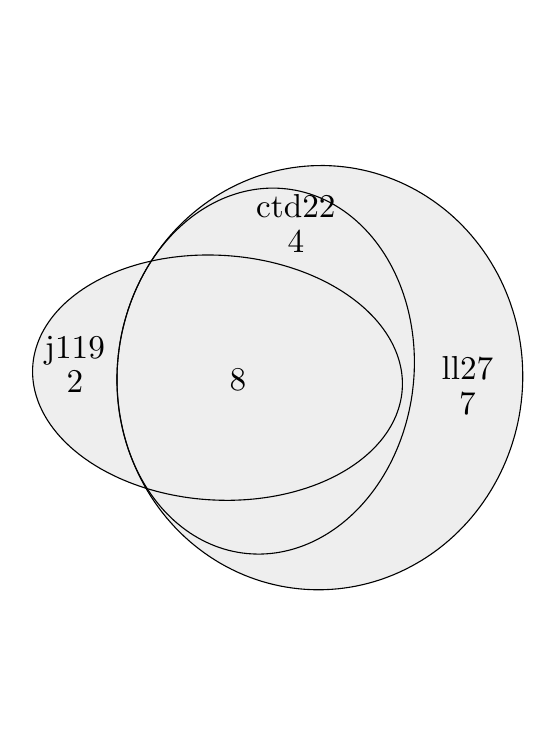
\begin{tikzpicture}[x=1pt,y=1pt]
\definecolor{fillColor}{RGB}{255,255,255}
\path[use as bounding box,fill=fillColor,fill opacity=0.00] (0,0) rectangle (180.67,252.94);
\begin{scope}
\path[clip] (  0.00,  0.00) rectangle (180.67,252.94);
\definecolor{fillColor}{RGB}{238,238,238}

\path[fill=fillColor,nonzero rule]
	( 42.04, 87.76) --
	( 40.92, 89.87) --
	( 39.86, 92.01) --
	( 38.87, 94.19) --
	( 37.94, 96.40) --
	( 37.59, 97.30) --
	( 37.29, 98.07) --
	( 36.59, 99.93) --
	( 35.95,101.82) --
	( 35.36,103.74) --
	( 34.82,105.68) --
	( 34.33,107.65) --
	( 33.89,109.64) --
	( 33.50,111.65) --
	( 33.16,113.67) --
	( 32.88,115.71) --
	( 32.65,117.76) --
	( 32.47,119.82) --
	( 32.35,121.90) --
	( 32.28,123.98) --
	( 32.26,126.06) --
	( 32.28,126.91) --
	( 32.28,127.03) --
	( 32.29,127.25) --
	( 32.30,128.15) --
	( 32.33,128.84) --
	( 32.35,129.45) --
	( 32.38,130.01) --
	( 32.39,130.23) --
	( 32.42,130.59) --
	( 32.49,131.87) --
	( 32.71,134.28) --
	( 33.00,136.68) --
	( 33.36,139.08) --
	( 33.79,141.46) --
	( 34.30,143.82) --
	( 34.88,146.17) --
	( 35.52,148.50) --
	( 35.88,149.65) --
	( 36.20,150.69) --
	( 36.22,150.74) --
	( 36.24,150.81) --
	( 36.34,151.09) --
	( 36.86,152.65) --
	( 37.01,153.06) --
	( 37.02,153.09) --
	( 37.05,153.15) --
	( 37.57,154.59) --
	( 38.33,156.50) --
	( 39.14,158.38) --
	( 40.00,160.23) --
	( 40.89,162.05) --
	( 41.84,163.84) --
	( 41.91,163.97) --
	( 41.96,164.06) --
	( 43.14,166.15) --
	( 44.38,168.20) --
	( 44.64,168.60) --
	( 44.36,168.54) --
	( 42.41,168.08) --
	( 40.48,167.58) --
	( 38.58,167.03) --
	( 36.71,166.45) --
	( 34.87,165.82) --
	( 33.07,165.16) --
	( 31.30,164.45) --
	( 29.57,163.71) --
	( 27.87,162.94) --
	( 26.22,162.12) --
	( 24.61,161.27) --
	( 23.05,160.39) --
	( 21.52,159.47) --
	( 20.05,158.52) --
	( 18.63,157.54) --
	( 17.25,156.52) --
	( 15.93,155.48) --
	( 14.65,154.41) --
	( 13.43,153.31) --
	( 12.27,152.18) --
	( 11.16,151.03) --
	( 10.11,149.85) --
	(  9.12,148.65) --
	(  8.19,147.43) --
	(  7.32,146.18) --
	(  6.51,144.92) --
	(  5.76,143.64) --
	(  5.07,142.34) --
	(  4.45,141.03) --
	(  3.89,139.70) --
	(  3.40,138.35) --
	(  2.97,137.00) --
	(  2.60,135.64) --
	(  2.30,134.26) --
	(  2.07,132.88) --
	(  1.90,131.49) --
	(  1.80,130.10) --
	(  1.77,128.70) --
	(  1.80,127.31) --
	(  1.90,125.91) --
	(  2.07,124.51) --
	(  2.30,123.11) --
	(  2.60,121.72) --
	(  2.97,120.33) --
	(  3.40,118.94) --
	(  3.89,117.57) --
	(  4.45,116.20) --
	(  5.08,114.85) --
	(  5.76,113.50) --
	(  6.51,112.17) --
	(  7.32,110.85) --
	(  8.20,109.55) --
	(  9.13,108.27) --
	( 10.12,107.00) --
	( 11.17,105.75) --
	( 12.28,104.53) --
	( 13.44,103.32) --
	( 14.66,102.14) --
	( 15.93,100.98) --
	( 17.26, 99.85) --
	( 18.64, 98.74) --
	( 20.06, 97.67) --
	( 21.54, 96.62) --
	( 23.06, 95.60) --
	( 24.62, 94.61) --
	( 26.23, 93.65) --
	( 27.89, 92.73) --
	( 29.58, 91.84) --
	( 31.31, 90.98) --
	( 33.08, 90.16) --
	( 34.88, 89.38) --
	( 36.72, 88.63) --
	( 38.59, 87.92) --
	( 40.49, 87.25) --
	( 42.42, 86.61) --
	( 42.75, 86.51) --
	cycle;

\path[fill=fillColor,nonzero rule]
	(107.40, 49.86) --
	(109.72, 49.98) --
	(112.03, 50.17) --
	(114.33, 50.44) --
	(116.62, 50.78) --
	(118.91, 51.20) --
	(121.17, 51.70) --
	(123.43, 52.26) --
	(125.66, 52.91) --
	(127.88, 53.62) --
	(130.07, 54.41) --
	(132.24, 55.27) --
	(134.39, 56.21) --
	(136.50, 57.21) --
	(138.58, 58.28) --
	(140.63, 59.42) --
	(142.65, 60.62) --
	(144.63, 61.89) --
	(146.57, 63.23) --
	(148.47, 64.63) --
	(150.32, 66.09) --
	(152.13, 67.61) --
	(153.90, 69.19) --
	(155.62, 70.83) --
	(157.28, 72.52) --
	(158.90, 74.26) --
	(160.46, 76.06) --
	(161.97, 77.91) --
	(163.42, 79.81) --
	(164.81, 81.75) --
	(166.15, 83.74) --
	(167.42, 85.77) --
	(168.63, 87.84) --
	(169.78, 89.95) --
	(170.87, 92.09) --
	(171.89, 94.27) --
	(172.85, 96.48) --
	(173.73, 98.72) --
	(174.55,100.99) --
	(175.30,103.29) --
	(175.99,105.61) --
	(176.60,107.95) --
	(177.14,110.30) --
	(177.61,112.68) --
	(178.00,115.06) --
	(178.33,117.46) --
	(178.58,119.87) --
	(178.76,122.28) --
	(178.87,124.70) --
	(178.90,127.12) --
	(178.86,129.54) --
	(178.75,131.96) --
	(178.57,134.37) --
	(178.31,136.77) --
	(177.98,139.16) --
	(177.58,141.54) --
	(177.10,143.91) --
	(176.56,146.26) --
	(175.94,148.58) --
	(175.25,150.89) --
	(174.50,153.17) --
	(173.67,155.43) --
	(172.78,157.65) --
	(171.82,159.85) --
	(170.80,162.01) --
	(169.71,164.14) --
	(168.55,166.22) --
	(167.33,168.27) --
	(166.06,170.28) --
	(164.72,172.24) --
	(163.32,174.16) --
	(161.86,176.03) --
	(160.35,177.85) --
	(158.79,179.62) --
	(157.17,181.34) --
	(155.50,183.00) --
	(153.78,184.61) --
	(152.01,186.16) --
	(150.19,187.65) --
	(148.33,189.07) --
	(146.43,190.44) --
	(144.49,191.74) --
	(142.51,192.98) --
	(140.49,194.15) --
	(138.44,195.25) --
	(136.35,196.28) --
	(134.24,197.25) --
	(132.09,198.14) --
	(129.92,198.96) --
	(127.73,199.71) --
	(125.51,200.39) --
	(123.27,201.00) --
	(121.02,201.52) --
	(118.75,201.98) --
	(116.46,202.36) --
	(114.17,202.66) --
	(111.86,202.89) --
	(109.56,203.04) --
	(107.24,203.12) --
	(104.93,203.11) --
	(102.61,203.04) --
	(100.30,202.88) --
	( 98.00,202.65) --
	( 95.70,202.35) --
	( 93.41,201.96) --
	( 91.13,201.51) --
	( 88.87,200.97) --
	( 86.63,200.37) --
	( 84.40,199.69) --
	( 82.20,198.94) --
	( 80.01,198.11) --
	( 77.86,197.21) --
	( 75.73,196.25) --
	( 73.63,195.21) --
	( 71.56,194.11) --
	( 69.53,192.93) --
	( 67.53,191.69) --
	( 65.57,190.39) --
	( 63.65,189.02) --
	( 61.78,187.59) --
	( 59.94,186.10) --
	( 58.15,184.55) --
	( 56.41,182.94) --
	( 54.72,181.28) --
	( 53.08,179.56) --
	( 51.49,177.79) --
	( 49.95,175.97) --
	( 48.48,174.09) --
	( 47.05,172.17) --
	( 45.69,170.21) --
	( 44.64,168.60) --
	( 44.69,168.61) --
	( 44.93,168.99) --
	( 46.05,170.63) --
	( 47.20,172.23) --
	( 48.39,173.78) --
	( 49.63,175.29) --
	( 50.89,176.75) --
	( 52.19,178.17) --
	( 53.53,179.53) --
	( 54.90,180.85) --
	( 56.30,182.11) --
	( 57.73,183.32) --
	( 59.18,184.48) --
	( 60.67,185.58) --
	( 62.17,186.62) --
	( 63.71,187.61) --
	( 65.26,188.53) --
	( 66.84,189.40) --
	( 68.43,190.21) --
	( 70.04,190.96) --
	( 71.67,191.64) --
	( 73.31,192.26) --
	( 74.97,192.82) --
	( 76.63,193.32) --
	( 78.31,193.75) --
	( 79.99,194.11) --
	( 81.68,194.42) --
	( 83.37,194.65) --
	( 85.07,194.82) --
	( 86.77,194.93) --
	( 88.46,194.96) --
	( 90.16,194.94) --
	( 91.84,194.84) --
	( 93.53,194.68) --
	( 95.20,194.46) --
	( 96.87,194.17) --
	( 98.53,193.81) --
	(100.17,193.39) --
	(101.80,192.91) --
	(103.41,192.36) --
	(105.01,191.75) --
	(106.59,191.07) --
	(108.14,190.34) --
	(109.68,189.54) --
	(111.19,188.68) --
	(112.68,187.76) --
	(114.14,186.79) --
	(115.57,185.75) --
	(116.97,184.66) --
	(118.34,183.52) --
	(119.68,182.31) --
	(120.98,181.06) --
	(122.25,179.75) --
	(123.49,178.40) --
	(124.69,176.99) --
	(125.84,175.54) --
	(126.96,174.03) --
	(128.04,172.49) --
	(129.08,170.90) --
	(130.07,169.27) --
	(131.02,167.59) --
	(131.92,165.88) --
	(132.78,164.14) --
	(133.59,162.35) --
	(134.36,160.54) --
	(135.07,158.69) --
	(135.74,156.81) --
	(136.36,154.91) --
	(136.93,152.98) --
	(137.44,151.02) --
	(137.91,149.04) --
	(138.32,147.04) --
	(138.68,145.03) --
	(138.99,143.00) --
	(139.25,140.95) --
	(139.45,138.89) --
	(139.60,136.83) --
	(139.70,134.75) --
	(139.74,132.67) --
	(139.73,130.58) --
	(139.67,128.49) --
	(139.55,126.41) --
	(139.38,124.32) --
	(139.15,122.24) --
	(138.88,120.17) --
	(138.55,118.10) --
	(138.16,116.05) --
	(137.73,114.01) --
	(137.24,111.98) --
	(136.71,109.97) --
	(136.12,107.98) --
	(135.48,106.01) --
	(134.79,104.06) --
	(134.06,102.14) --
	(133.27,100.24) --
	(132.44, 98.37) --
	(131.57, 96.54) --
	(130.65, 94.73) --
	(129.68, 92.96) --
	(128.67, 91.23) --
	(127.62, 89.53) --
	(126.52, 87.87) --
	(125.39, 86.25) --
	(124.21, 84.68) --
	(123.00, 83.14) --
	(121.75, 81.66) --
	(120.47, 80.22) --
	(119.15, 78.83) --
	(117.80, 77.49) --
	(116.41, 76.20) --
	(115.00, 74.96) --
	(113.56, 73.78) --
	(112.09, 72.65) --
	(110.59, 71.58) --
	(109.07, 70.56) --
	(107.53, 69.61) --
	(105.96, 68.71) --
	(104.38, 67.87) --
	(102.77, 67.09) --
	(101.15, 66.38) --
	( 99.52, 65.72) --
	( 97.87, 65.13) --
	( 96.21, 64.61) --
	( 94.54, 64.14) --
	( 92.86, 63.75) --
	( 91.17, 63.41) --
	( 89.48, 63.14) --
	( 87.79, 62.94) --
	( 86.09, 62.80) --
	( 84.39, 62.73) --
	( 82.70, 62.73) --
	( 81.01, 62.79) --
	( 79.32, 62.91) --
	( 77.64, 63.11) --
	( 75.97, 63.36) --
	( 74.31, 63.69) --
	( 72.66, 64.07) --
	( 71.02, 64.53) --
	( 69.40, 65.04) --
	( 67.79, 65.62) --
	( 66.21, 66.27) --
	( 64.64, 66.97) --
	( 63.09, 67.74) --
	( 61.57, 68.57) --
	( 60.07, 69.45) --
	( 58.60, 70.40) --
	( 57.15, 71.41) --
	( 55.74, 72.47) --
	( 54.35, 73.59) --
	( 52.99, 74.76) --
	( 51.67, 75.99) --
	( 50.38, 77.27) --
	( 49.13, 78.60) --
	( 47.91, 79.99) --
	( 46.74, 81.42) --
	( 45.60, 82.89) --
	( 44.50, 84.42) --
	( 43.44, 85.99) --
	( 43.20, 86.38) --
	( 42.75, 86.51) --
	( 43.22, 85.69) --
	( 44.47, 83.66) --
	( 45.78, 81.68) --
	( 47.15, 79.74) --
	( 48.58, 77.84) --
	( 50.06, 75.99) --
	( 51.60, 74.20) --
	( 53.19, 72.45) --
	( 54.84, 70.76) --
	( 56.53, 69.13) --
	( 58.28, 67.55) --
	( 60.07, 66.03) --
	( 61.91, 64.58) --
	( 63.79, 63.18) --
	( 65.71, 61.85) --
	( 67.67, 60.58) --
	( 69.67, 59.37) --
	( 71.71, 58.24) --
	( 73.78, 57.17) --
	( 75.88, 56.17) --
	( 78.01, 55.24) --
	( 80.17, 54.38) --
	( 82.35, 53.60) --
	( 84.56, 52.88) --
	( 86.78, 52.24) --
	( 89.03, 51.68) --
	( 91.29, 51.18) --
	( 93.57, 50.77) --
	( 95.86, 50.43) --
	( 98.16, 50.16) --
	(100.46, 49.97) --
	(102.78, 49.86) --
	(105.09, 49.82) --
	cycle;

\path[fill=fillColor,nonzero rule]
	( 42.83,165.60) --
	( 43.86,167.31) --
	( 44.69,168.61) --
	( 44.64,168.60) --
	( 44.38,168.20) --
	( 43.14,166.15) --
	( 41.96,164.06) --
	( 41.91,163.97) --
	cycle
	( 37.05,153.15) --
	( 37.02,153.09) --
	( 37.01,153.06) --
	cycle
	( 36.34,151.09) --
	( 36.24,150.81) --
	( 36.22,150.74) --
	cycle
	( 32.54,132.32) --
	( 32.74,134.40) --
	( 32.99,136.48) --
	( 33.29,138.55) --
	( 33.65,140.61) --
	( 34.05,142.66) --
	( 34.51,144.69) --
	( 35.03,146.71) --
	( 35.59,148.71) --
	( 35.88,149.65) --
	( 35.52,148.50) --
	( 34.88,146.17) --
	( 34.30,143.82) --
	( 33.79,141.46) --
	( 33.36,139.08) --
	( 33.00,136.68) --
	( 32.71,134.28) --
	( 32.49,131.87) --
	( 32.42,130.59) --
	cycle
	( 32.38,130.01) --
	( 32.35,129.45) --
	( 32.33,128.84) --
	cycle
	( 32.29,127.25) --
	( 32.28,127.03) --
	( 32.28,126.91) --
	cycle
	( 42.43, 87.60) --
	( 41.46, 89.25) --
	( 40.53, 90.94) --
	( 39.65, 92.67) --
	( 38.81, 94.44) --
	( 38.03, 96.24) --
	( 37.59, 97.30) --
	( 37.94, 96.40) --
	( 38.87, 94.19) --
	( 39.86, 92.01) --
	( 40.92, 89.87) --
	( 42.04, 87.76) --
	( 42.75, 86.51) --
	( 43.20, 86.38) --
	cycle;

\path[fill=fillColor,nonzero rule]
	( 37.88,155.35) --
	( 38.80,157.57) --
	( 39.79,159.77) --
	( 40.84,161.93) --
	( 41.91,163.97) --
	( 41.84,163.84) --
	( 40.89,162.05) --
	( 40.00,160.23) --
	( 39.14,158.38) --
	( 38.33,156.50) --
	( 37.57,154.59) --
	( 37.05,153.15) --
	cycle
	( 37.01,153.06) --
	( 36.86,152.65) --
	( 36.34,151.09) --
	cycle
	( 36.22,150.74) --
	( 36.20,150.69) --
	( 35.88,149.65) --
	cycle
	( 32.42,130.59) --
	( 32.39,130.23) --
	( 32.38,130.01) --
	cycle
	( 32.33,128.84) --
	( 32.30,128.15) --
	( 32.29,127.25) --
	cycle
	( 37.08, 98.64) --
	( 36.29,100.91) --
	( 35.57,103.20) --
	( 34.92,105.52) --
	( 34.34,107.86) --
	( 33.83,110.22) --
	( 33.39,112.59) --
	( 33.02,114.98) --
	( 32.73,117.37) --
	( 32.51,119.78) --
	( 32.36,122.20) --
	( 32.28,124.61) --
	( 32.28,126.91) --
	( 32.26,126.06) --
	( 32.28,123.98) --
	( 32.35,121.90) --
	( 32.47,119.82) --
	( 32.65,117.76) --
	( 32.88,115.71) --
	( 33.16,113.67) --
	( 33.50,111.65) --
	( 33.89,109.64) --
	( 34.33,107.65) --
	( 34.82,105.68) --
	( 35.36,103.74) --
	( 35.95,101.82) --
	( 36.59, 99.93) --
	( 37.29, 98.07) --
	( 37.59, 97.30) --
	cycle;

\path[fill=fillColor,nonzero rule]
	( 84.39, 62.73) --
	( 86.09, 62.80) --
	( 87.79, 62.94) --
	( 89.48, 63.14) --
	( 91.17, 63.41) --
	( 92.86, 63.75) --
	( 94.54, 64.14) --
	( 96.21, 64.61) --
	( 97.87, 65.13) --
	( 99.52, 65.72) --
	(101.15, 66.38) --
	(102.77, 67.09) --
	(104.38, 67.87) --
	(105.96, 68.71) --
	(107.53, 69.61) --
	(109.07, 70.56) --
	(110.59, 71.58) --
	(112.09, 72.65) --
	(113.56, 73.78) --
	(115.00, 74.96) --
	(116.41, 76.20) --
	(117.80, 77.49) --
	(119.15, 78.83) --
	(120.47, 80.22) --
	(121.75, 81.66) --
	(123.00, 83.14) --
	(124.21, 84.68) --
	(125.39, 86.25) --
	(126.52, 87.87) --
	(127.62, 89.53) --
	(128.67, 91.23) --
	(129.68, 92.96) --
	(130.65, 94.73) --
	(131.57, 96.54) --
	(132.44, 98.37) --
	(133.27,100.24) --
	(134.06,102.14) --
	(134.79,104.06) --
	(135.48,106.01) --
	(136.12,107.98) --
	(136.71,109.97) --
	(137.24,111.98) --
	(137.73,114.01) --
	(138.16,116.05) --
	(138.55,118.10) --
	(138.88,120.17) --
	(139.15,122.24) --
	(139.38,124.32) --
	(139.55,126.41) --
	(139.67,128.49) --
	(139.73,130.58) --
	(139.74,132.67) --
	(139.70,134.75) --
	(139.60,136.83) --
	(139.45,138.89) --
	(139.25,140.95) --
	(138.99,143.00) --
	(138.68,145.03) --
	(138.32,147.04) --
	(137.91,149.04) --
	(137.44,151.02) --
	(136.93,152.98) --
	(136.36,154.91) --
	(135.74,156.81) --
	(135.07,158.69) --
	(134.36,160.54) --
	(133.59,162.35) --
	(132.78,164.14) --
	(131.92,165.88) --
	(131.02,167.59) --
	(130.07,169.27) --
	(129.08,170.90) --
	(128.04,172.49) --
	(126.96,174.03) --
	(125.84,175.54) --
	(124.69,176.99) --
	(123.49,178.40) --
	(122.25,179.75) --
	(120.98,181.06) --
	(119.68,182.31) --
	(118.34,183.52) --
	(116.97,184.66) --
	(115.57,185.75) --
	(114.14,186.79) --
	(112.68,187.76) --
	(111.19,188.68) --
	(109.68,189.54) --
	(108.14,190.34) --
	(106.59,191.07) --
	(105.01,191.75) --
	(103.41,192.36) --
	(101.80,192.91) --
	(100.17,193.39) --
	( 98.53,193.81) --
	( 96.87,194.17) --
	( 95.20,194.46) --
	( 93.53,194.68) --
	( 91.84,194.84) --
	( 90.16,194.94) --
	( 88.46,194.96) --
	( 86.77,194.93) --
	( 85.07,194.82) --
	( 83.37,194.65) --
	( 81.68,194.42) --
	( 79.99,194.11) --
	( 78.31,193.75) --
	( 76.63,193.32) --
	( 74.97,192.82) --
	( 73.31,192.26) --
	( 71.67,191.64) --
	( 70.04,190.96) --
	( 68.43,190.21) --
	( 66.84,189.40) --
	( 65.26,188.53) --
	( 63.71,187.61) --
	( 62.17,186.62) --
	( 60.67,185.58) --
	( 59.18,184.48) --
	( 57.73,183.32) --
	( 56.30,182.11) --
	( 54.90,180.85) --
	( 53.53,179.53) --
	( 52.19,178.17) --
	( 50.89,176.75) --
	( 49.63,175.29) --
	( 48.39,173.78) --
	( 47.20,172.23) --
	( 46.05,170.63) --
	( 44.93,168.99) --
	( 44.69,168.61) --
	( 46.34,168.96) --
	( 48.34,169.34) --
	( 50.36,169.67) --
	( 52.40,169.97) --
	( 54.45,170.21) --
	( 56.52,170.42) --
	( 58.60,170.58) --
	( 60.69,170.70) --
	( 62.79,170.77) --
	( 64.90,170.80) --
	( 67.00,170.78) --
	( 69.11,170.72) --
	( 71.22,170.62) --
	( 73.33,170.47) --
	( 75.43,170.28) --
	( 77.53,170.05) --
	( 79.61,169.77) --
	( 81.69,169.45) --
	( 83.75,169.08) --
	( 85.80,168.68) --
	( 87.83,168.23) --
	( 89.84,167.74) --
	( 91.83,167.20) --
	( 93.79,166.63) --
	( 95.73,166.02) --
	( 97.65,165.37) --
	( 99.53,164.68) --
	(101.39,163.95) --
	(103.21,163.18) --
	(105.00,162.38) --
	(106.75,161.54) --
	(108.46,160.67) --
	(110.13,159.76) --
	(111.76,158.82) --
	(113.35,157.85) --
	(114.90,156.84) --
	(116.39,155.81) --
	(117.84,154.74) --
	(119.25,153.65) --
	(120.60,152.53) --
	(121.90,151.39) --
	(123.14,150.22) --
	(124.33,149.02) --
	(125.47,147.81) --
	(126.55,146.57) --
	(127.57,145.31) --
	(128.53,144.04) --
	(129.43,142.74) --
	(130.28,141.44) --
	(131.06,140.11) --
	(131.77,138.77) --
	(132.43,137.42) --
	(133.02,136.06) --
	(133.55,134.69) --
	(134.01,133.31) --
	(134.41,131.92) --
	(134.74,130.53) --
	(135.01,129.14) --
	(135.21,127.74) --
	(135.34,126.34) --
	(135.41,124.94) --
	(135.41,123.54) --
	(135.34,122.15) --
	(135.21,120.76) --
	(135.01,119.37) --
	(134.74,117.99) --
	(134.41,116.63) --
	(134.01,115.27) --
	(133.55,113.92) --
	(133.03,112.58) --
	(132.43,111.26) --
	(131.78,109.95) --
	(131.06,108.66) --
	(130.28,107.39) --
	(129.44,106.14) --
	(128.54,104.90) --
	(127.58,103.69) --
	(126.55,102.50) --
	(125.48,101.34) --
	(124.34,100.20) --
	(123.15, 99.08) --
	(121.90, 98.00) --
	(120.61, 96.94) --
	(119.26, 95.91) --
	(117.85, 94.91) --
	(116.40, 93.94) --
	(114.91, 93.01) --
	(113.36, 92.11) --
	(111.78, 91.24) --
	(110.14, 90.41) --
	(108.47, 89.61) --
	(106.76, 88.86) --
	(105.01, 88.13) --
	(103.22, 87.45) --
	(101.40, 86.81) --
	( 99.55, 86.20) --
	( 97.66, 85.64) --
	( 95.75, 85.11) --
	( 93.81, 84.63) --
	( 91.84, 84.19) --
	( 89.85, 83.79) --
	( 87.84, 83.43) --
	( 85.81, 83.12) --
	( 83.76, 82.85) --
	( 81.70, 82.62) --
	( 79.63, 82.44) --
	( 77.54, 82.30) --
	( 75.45, 82.21) --
	( 73.34, 82.15) --
	( 71.24, 82.15) --
	( 69.13, 82.19) --
	( 67.02, 82.27) --
	( 64.91, 82.39) --
	( 62.81, 82.56) --
	( 60.71, 82.77) --
	( 58.62, 83.03) --
	( 56.54, 83.33) --
	( 54.47, 83.68) --
	( 52.41, 84.06) --
	( 50.37, 84.49) --
	( 48.35, 84.96) --
	( 46.35, 85.47) --
	( 44.37, 86.02) --
	( 43.20, 86.38) --
	( 43.44, 85.99) --
	( 44.50, 84.42) --
	( 45.60, 82.89) --
	( 46.74, 81.42) --
	( 47.91, 79.99) --
	( 49.13, 78.60) --
	( 50.38, 77.27) --
	( 51.67, 75.99) --
	( 52.99, 74.76) --
	( 54.35, 73.59) --
	( 55.74, 72.47) --
	( 57.15, 71.41) --
	( 58.60, 70.40) --
	( 60.07, 69.45) --
	( 61.57, 68.57) --
	( 63.09, 67.74) --
	( 64.64, 66.97) --
	( 66.21, 66.27) --
	( 67.79, 65.62) --
	( 69.40, 65.04) --
	( 71.02, 64.53) --
	( 72.66, 64.07) --
	( 74.31, 63.69) --
	( 75.97, 63.36) --
	( 77.64, 63.11) --
	( 79.32, 62.91) --
	( 81.01, 62.79) --
	( 82.70, 62.73) --
	cycle;

\path[fill=fillColor,nonzero rule]
	( 73.34, 82.15) --
	( 75.45, 82.21) --
	( 77.54, 82.30) --
	( 79.63, 82.44) --
	( 81.70, 82.62) --
	( 83.76, 82.85) --
	( 85.81, 83.12) --
	( 87.84, 83.43) --
	( 89.85, 83.79) --
	( 91.84, 84.19) --
	( 93.81, 84.63) --
	( 95.75, 85.11) --
	( 97.66, 85.64) --
	( 99.55, 86.20) --
	(101.40, 86.81) --
	(103.22, 87.45) --
	(105.01, 88.13) --
	(106.76, 88.86) --
	(108.47, 89.61) --
	(110.14, 90.41) --
	(111.78, 91.24) --
	(113.36, 92.11) --
	(114.91, 93.01) --
	(116.40, 93.94) --
	(117.85, 94.91) --
	(119.26, 95.91) --
	(120.61, 96.94) --
	(121.90, 98.00) --
	(123.15, 99.08) --
	(124.34,100.20) --
	(125.48,101.34) --
	(126.55,102.50) --
	(127.58,103.69) --
	(128.54,104.90) --
	(129.44,106.14) --
	(130.28,107.39) --
	(131.06,108.66) --
	(131.78,109.95) --
	(132.43,111.26) --
	(133.03,112.58) --
	(133.55,113.92) --
	(134.01,115.27) --
	(134.41,116.63) --
	(134.74,117.99) --
	(135.01,119.37) --
	(135.21,120.76) --
	(135.34,122.15) --
	(135.41,123.54) --
	(135.41,124.94) --
	(135.34,126.34) --
	(135.21,127.74) --
	(135.01,129.14) --
	(134.74,130.53) --
	(134.41,131.92) --
	(134.01,133.31) --
	(133.55,134.69) --
	(133.02,136.06) --
	(132.43,137.42) --
	(131.77,138.77) --
	(131.06,140.11) --
	(130.28,141.44) --
	(129.43,142.74) --
	(128.53,144.04) --
	(127.57,145.31) --
	(126.55,146.57) --
	(125.47,147.81) --
	(124.33,149.02) --
	(123.14,150.22) --
	(121.90,151.39) --
	(120.60,152.53) --
	(119.25,153.65) --
	(117.84,154.74) --
	(116.39,155.81) --
	(114.90,156.84) --
	(113.35,157.85) --
	(111.76,158.82) --
	(110.13,159.76) --
	(108.46,160.67) --
	(106.75,161.54) --
	(105.00,162.38) --
	(103.21,163.18) --
	(101.39,163.95) --
	( 99.53,164.68) --
	( 97.65,165.37) --
	( 95.73,166.02) --
	( 93.79,166.63) --
	( 91.83,167.20) --
	( 89.84,167.74) --
	( 87.83,168.23) --
	( 85.80,168.68) --
	( 83.75,169.08) --
	( 81.69,169.45) --
	( 79.61,169.77) --
	( 77.53,170.05) --
	( 75.43,170.28) --
	( 73.33,170.47) --
	( 71.22,170.62) --
	( 69.11,170.72) --
	( 67.00,170.78) --
	( 64.90,170.80) --
	( 62.79,170.77) --
	( 60.69,170.70) --
	( 58.60,170.58) --
	( 56.52,170.42) --
	( 54.45,170.21) --
	( 52.40,169.97) --
	( 50.36,169.67) --
	( 48.34,169.34) --
	( 46.34,168.96) --
	( 44.69,168.61) --
	( 43.86,167.31) --
	( 42.83,165.60) --
	( 41.91,163.97) --
	( 40.84,161.93) --
	( 39.79,159.77) --
	( 38.80,157.57) --
	( 37.88,155.35) --
	( 37.05,153.15) --
	( 37.01,153.06) --
	( 36.34,151.09) --
	( 36.22,150.74) --
	( 35.88,149.65) --
	( 35.59,148.71) --
	( 35.03,146.71) --
	( 34.51,144.69) --
	( 34.05,142.66) --
	( 33.65,140.61) --
	( 33.29,138.55) --
	( 32.99,136.48) --
	( 32.74,134.40) --
	( 32.54,132.32) --
	( 32.42,130.59) --
	( 32.38,130.01) --
	( 32.33,128.84) --
	( 32.29,127.25) --
	( 32.28,126.91) --
	( 32.28,124.61) --
	( 32.36,122.20) --
	( 32.51,119.78) --
	( 32.73,117.37) --
	( 33.02,114.98) --
	( 33.39,112.59) --
	( 33.83,110.22) --
	( 34.34,107.86) --
	( 34.92,105.52) --
	( 35.57,103.20) --
	( 36.29,100.91) --
	( 37.08, 98.64) --
	( 37.59, 97.30) --
	( 38.03, 96.24) --
	( 38.81, 94.44) --
	( 39.65, 92.67) --
	( 40.53, 90.94) --
	( 41.46, 89.25) --
	( 42.43, 87.60) --
	( 43.20, 86.38) --
	( 44.37, 86.02) --
	( 46.35, 85.47) --
	( 48.35, 84.96) --
	( 50.37, 84.49) --
	( 52.41, 84.06) --
	( 54.47, 83.68) --
	( 56.54, 83.33) --
	( 58.62, 83.03) --
	( 60.71, 82.77) --
	( 62.81, 82.56) --
	( 64.91, 82.39) --
	( 67.02, 82.27) --
	( 69.13, 82.19) --
	( 71.24, 82.15) --
	cycle;
\definecolor{drawColor}{RGB}{0,0,0}

\path[draw=drawColor,line width= 0.4pt,line join=round,line cap=round] ( 71.22,170.62) --
	( 69.11,170.72) --
	( 67.00,170.78) --
	( 64.90,170.80) --
	( 62.79,170.77) --
	( 60.69,170.70) --
	( 58.60,170.58) --
	( 56.52,170.42) --
	( 54.45,170.21) --
	( 52.40,169.97) --
	( 50.36,169.67) --
	( 48.34,169.34) --
	( 46.34,168.96) --
	( 44.36,168.54) --
	( 42.41,168.08) --
	( 40.48,167.58) --
	( 38.58,167.03) --
	( 36.71,166.45) --
	( 34.87,165.82) --
	( 33.07,165.16) --
	( 31.30,164.45) --
	( 29.57,163.71) --
	( 27.87,162.94) --
	( 26.22,162.12) --
	( 24.61,161.27) --
	( 23.05,160.39) --
	( 21.52,159.47) --
	( 20.05,158.52) --
	( 18.63,157.54) --
	( 17.25,156.52) --
	( 15.93,155.48) --
	( 14.65,154.41) --
	( 13.43,153.31) --
	( 12.27,152.18) --
	( 11.16,151.03) --
	( 10.11,149.85) --
	(  9.12,148.65) --
	(  8.19,147.43) --
	(  7.32,146.18) --
	(  6.51,144.92) --
	(  5.76,143.64) --
	(  5.07,142.34) --
	(  4.45,141.03) --
	(  3.89,139.70) --
	(  3.40,138.35) --
	(  2.97,137.00) --
	(  2.60,135.64) --
	(  2.30,134.26) --
	(  2.07,132.88) --
	(  1.90,131.49) --
	(  1.80,130.10) --
	(  1.77,128.70) --
	(  1.80,127.31) --
	(  1.90,125.91) --
	(  2.07,124.51) --
	(  2.30,123.11) --
	(  2.60,121.72) --
	(  2.97,120.33) --
	(  3.40,118.94) --
	(  3.89,117.57) --
	(  4.45,116.20) --
	(  5.08,114.85) --
	(  5.76,113.50) --
	(  6.51,112.17) --
	(  7.32,110.85) --
	(  8.20,109.55) --
	(  9.13,108.27) --
	( 10.12,107.00) --
	( 11.17,105.75) --
	( 12.28,104.53) --
	( 13.44,103.32) --
	( 14.66,102.14) --
	( 15.93,100.98) --
	( 17.26, 99.85) --
	( 18.64, 98.74) --
	( 20.06, 97.67) --
	( 21.54, 96.62) --
	( 23.06, 95.60) --
	( 24.62, 94.61) --
	( 26.23, 93.65) --
	( 27.89, 92.73) --
	( 29.58, 91.84) --
	( 31.31, 90.98) --
	( 33.08, 90.16) --
	( 34.88, 89.38) --
	( 36.72, 88.63) --
	( 38.59, 87.92) --
	( 40.49, 87.25) --
	( 42.42, 86.61) --
	( 44.37, 86.02) --
	( 46.35, 85.47) --
	( 48.35, 84.96) --
	( 50.37, 84.49) --
	( 52.41, 84.06) --
	( 54.47, 83.68) --
	( 56.54, 83.33) --
	( 58.62, 83.03) --
	( 60.71, 82.77) --
	( 62.81, 82.56) --
	( 64.91, 82.39) --
	( 67.02, 82.27) --
	( 69.13, 82.19) --
	( 71.24, 82.15) --
	( 73.34, 82.15) --
	( 75.45, 82.21) --
	( 77.54, 82.30) --
	( 79.63, 82.44) --
	( 81.70, 82.62) --
	( 83.76, 82.85) --
	( 85.81, 83.12) --
	( 87.84, 83.43) --
	( 89.85, 83.79) --
	( 91.84, 84.19) --
	( 93.81, 84.63) --
	( 95.75, 85.11) --
	( 97.66, 85.64) --
	( 99.55, 86.20) --
	(101.40, 86.81) --
	(103.22, 87.45) --
	(105.01, 88.13) --
	(106.76, 88.86) --
	(108.47, 89.61) --
	(110.14, 90.41) --
	(111.78, 91.24) --
	(113.36, 92.11) --
	(114.91, 93.01) --
	(116.40, 93.94) --
	(117.85, 94.91) --
	(119.26, 95.91) --
	(120.61, 96.94) --
	(121.90, 98.00) --
	(123.15, 99.08) --
	(124.34,100.20) --
	(125.48,101.34) --
	(126.55,102.50) --
	(127.58,103.69) --
	(128.54,104.90) --
	(129.44,106.14) --
	(130.28,107.39) --
	(131.06,108.66) --
	(131.78,109.95) --
	(132.43,111.26) --
	(133.03,112.58) --
	(133.55,113.92) --
	(134.01,115.27) --
	(134.41,116.63) --
	(134.74,117.99) --
	(135.01,119.37) --
	(135.21,120.76) --
	(135.34,122.15) --
	(135.41,123.54) --
	(135.41,124.94) --
	(135.34,126.34) --
	(135.21,127.74) --
	(135.01,129.14) --
	(134.74,130.53) --
	(134.41,131.92) --
	(134.01,133.31) --
	(133.55,134.69) --
	(133.02,136.06) --
	(132.43,137.42) --
	(131.77,138.77) --
	(131.06,140.11) --
	(130.28,141.44) --
	(129.43,142.74) --
	(128.53,144.04) --
	(127.57,145.31) --
	(126.55,146.57) --
	(125.47,147.81) --
	(124.33,149.02) --
	(123.14,150.22) --
	(121.90,151.39) --
	(120.60,152.53) --
	(119.25,153.65) --
	(117.84,154.74) --
	(116.39,155.81) --
	(114.90,156.84) --
	(113.35,157.85) --
	(111.76,158.82) --
	(110.13,159.76) --
	(108.46,160.67) --
	(106.75,161.54) --
	(105.00,162.38) --
	(103.21,163.18) --
	(101.39,163.95) --
	( 99.53,164.68) --
	( 97.65,165.37) --
	( 95.73,166.02) --
	( 93.79,166.63) --
	( 91.83,167.20) --
	( 89.84,167.74) --
	( 87.83,168.23) --
	( 85.80,168.68) --
	( 83.75,169.08) --
	( 81.69,169.45) --
	( 79.61,169.77) --
	( 77.53,170.05) --
	( 75.43,170.28) --
	( 73.33,170.47) --
	( 71.22,170.62);

\path[draw=drawColor,line width= 0.4pt,line join=round,line cap=round] (111.86,202.89) --
	(109.56,203.04) --
	(107.24,203.12) --
	(104.93,203.11) --
	(102.61,203.04) --
	(100.30,202.88) --
	( 98.00,202.65) --
	( 95.70,202.35) --
	( 93.41,201.96) --
	( 91.13,201.51) --
	( 88.87,200.97) --
	( 86.63,200.37) --
	( 84.40,199.69) --
	( 82.20,198.94) --
	( 80.01,198.11) --
	( 77.86,197.21) --
	( 75.73,196.25) --
	( 73.63,195.21) --
	( 71.56,194.11) --
	( 69.53,192.93) --
	( 67.53,191.69) --
	( 65.57,190.39) --
	( 63.65,189.02) --
	( 61.78,187.59) --
	( 59.94,186.10) --
	( 58.15,184.55) --
	( 56.41,182.94) --
	( 54.72,181.28) --
	( 53.08,179.56) --
	( 51.49,177.79) --
	( 49.95,175.97) --
	( 48.48,174.09) --
	( 47.05,172.17) --
	( 45.69,170.21) --
	( 44.38,168.20) --
	( 43.14,166.15) --
	( 41.96,164.06) --
	( 40.84,161.93) --
	( 39.79,159.77) --
	( 38.80,157.57) --
	( 37.88,155.35) --
	( 37.02,153.09) --
	( 36.24,150.81) --
	( 35.52,148.50) --
	( 34.88,146.17) --
	( 34.30,143.82) --
	( 33.79,141.46) --
	( 33.36,139.08) --
	( 33.00,136.68) --
	( 32.71,134.28) --
	( 32.49,131.87) --
	( 32.35,129.45) --
	( 32.28,127.03) --
	( 32.28,124.61) --
	( 32.36,122.20) --
	( 32.51,119.78) --
	( 32.73,117.37) --
	( 33.02,114.98) --
	( 33.39,112.59) --
	( 33.83,110.22) --
	( 34.34,107.86) --
	( 34.92,105.52) --
	( 35.57,103.20) --
	( 36.29,100.91) --
	( 37.08, 98.64) --
	( 37.94, 96.40) --
	( 38.87, 94.19) --
	( 39.86, 92.01) --
	( 40.92, 89.87) --
	( 42.04, 87.76) --
	( 43.22, 85.69) --
	( 44.47, 83.66) --
	( 45.78, 81.68) --
	( 47.15, 79.74) --
	( 48.58, 77.84) --
	( 50.06, 75.99) --
	( 51.60, 74.20) --
	( 53.19, 72.45) --
	( 54.84, 70.76) --
	( 56.53, 69.13) --
	( 58.28, 67.55) --
	( 60.07, 66.03) --
	( 61.91, 64.58) --
	( 63.79, 63.18) --
	( 65.71, 61.85) --
	( 67.67, 60.58) --
	( 69.67, 59.37) --
	( 71.71, 58.24) --
	( 73.78, 57.17) --
	( 75.88, 56.17) --
	( 78.01, 55.24) --
	( 80.17, 54.38) --
	( 82.35, 53.60) --
	( 84.56, 52.88) --
	( 86.78, 52.24) --
	( 89.03, 51.68) --
	( 91.29, 51.18) --
	( 93.57, 50.77) --
	( 95.86, 50.43) --
	( 98.16, 50.16) --
	(100.46, 49.97) --
	(102.78, 49.86) --
	(105.09, 49.82) --
	(107.40, 49.86) --
	(109.72, 49.98) --
	(112.03, 50.17) --
	(114.33, 50.44) --
	(116.62, 50.78) --
	(118.91, 51.20) --
	(121.17, 51.70) --
	(123.43, 52.26) --
	(125.66, 52.91) --
	(127.88, 53.62) --
	(130.07, 54.41) --
	(132.24, 55.27) --
	(134.39, 56.21) --
	(136.50, 57.21) --
	(138.58, 58.28) --
	(140.63, 59.42) --
	(142.65, 60.62) --
	(144.63, 61.89) --
	(146.57, 63.23) --
	(148.47, 64.63) --
	(150.32, 66.09) --
	(152.13, 67.61) --
	(153.90, 69.19) --
	(155.62, 70.83) --
	(157.28, 72.52) --
	(158.90, 74.26) --
	(160.46, 76.06) --
	(161.97, 77.91) --
	(163.42, 79.81) --
	(164.81, 81.75) --
	(166.15, 83.74) --
	(167.42, 85.77) --
	(168.63, 87.84) --
	(169.78, 89.95) --
	(170.87, 92.09) --
	(171.89, 94.27) --
	(172.85, 96.48) --
	(173.73, 98.72) --
	(174.55,100.99) --
	(175.30,103.29) --
	(175.99,105.61) --
	(176.60,107.95) --
	(177.14,110.30) --
	(177.61,112.68) --
	(178.00,115.06) --
	(178.33,117.46) --
	(178.58,119.87) --
	(178.76,122.28) --
	(178.87,124.70) --
	(178.90,127.12) --
	(178.86,129.54) --
	(178.75,131.96) --
	(178.57,134.37) --
	(178.31,136.77) --
	(177.98,139.16) --
	(177.58,141.54) --
	(177.10,143.91) --
	(176.56,146.26) --
	(175.94,148.58) --
	(175.25,150.89) --
	(174.50,153.17) --
	(173.67,155.43) --
	(172.78,157.65) --
	(171.82,159.85) --
	(170.80,162.01) --
	(169.71,164.14) --
	(168.55,166.22) --
	(167.33,168.27) --
	(166.06,170.28) --
	(164.72,172.24) --
	(163.32,174.16) --
	(161.86,176.03) --
	(160.35,177.85) --
	(158.79,179.62) --
	(157.17,181.34) --
	(155.50,183.00) --
	(153.78,184.61) --
	(152.01,186.16) --
	(150.19,187.65) --
	(148.33,189.07) --
	(146.43,190.44) --
	(144.49,191.74) --
	(142.51,192.98) --
	(140.49,194.15) --
	(138.44,195.25) --
	(136.35,196.28) --
	(134.24,197.25) --
	(132.09,198.14) --
	(129.92,198.96) --
	(127.73,199.71) --
	(125.51,200.39) --
	(123.27,201.00) --
	(121.02,201.52) --
	(118.75,201.98) --
	(116.46,202.36) --
	(114.17,202.66) --
	(111.86,202.89);

\path[draw=drawColor,line width= 0.4pt,line join=round,line cap=round] ( 93.53,194.68) --
	( 91.84,194.84) --
	( 90.16,194.94) --
	( 88.46,194.96) --
	( 86.77,194.93) --
	( 85.07,194.82) --
	( 83.37,194.65) --
	( 81.68,194.42) --
	( 79.99,194.11) --
	( 78.31,193.75) --
	( 76.63,193.32) --
	( 74.97,192.82) --
	( 73.31,192.26) --
	( 71.67,191.64) --
	( 70.04,190.96) --
	( 68.43,190.21) --
	( 66.84,189.40) --
	( 65.26,188.53) --
	( 63.71,187.61) --
	( 62.17,186.62) --
	( 60.67,185.58) --
	( 59.18,184.48) --
	( 57.73,183.32) --
	( 56.30,182.11) --
	( 54.90,180.85) --
	( 53.53,179.53) --
	( 52.19,178.17) --
	( 50.89,176.75) --
	( 49.63,175.29) --
	( 48.39,173.78) --
	( 47.20,172.23) --
	( 46.05,170.63) --
	( 44.93,168.99) --
	( 43.86,167.31) --
	( 42.83,165.60) --
	( 41.84,163.84) --
	( 40.89,162.05) --
	( 40.00,160.23) --
	( 39.14,158.38) --
	( 38.33,156.50) --
	( 37.57,154.59) --
	( 36.86,152.65) --
	( 36.20,150.69) --
	( 35.59,148.71) --
	( 35.03,146.71) --
	( 34.51,144.69) --
	( 34.05,142.66) --
	( 33.65,140.61) --
	( 33.29,138.55) --
	( 32.99,136.48) --
	( 32.74,134.40) --
	( 32.54,132.32) --
	( 32.39,130.23) --
	( 32.30,128.15) --
	( 32.26,126.06) --
	( 32.28,123.98) --
	( 32.35,121.90) --
	( 32.47,119.82) --
	( 32.65,117.76) --
	( 32.88,115.71) --
	( 33.16,113.67) --
	( 33.50,111.65) --
	( 33.89,109.64) --
	( 34.33,107.65) --
	( 34.82,105.68) --
	( 35.36,103.74) --
	( 35.95,101.82) --
	( 36.59, 99.93) --
	( 37.29, 98.07) --
	( 38.03, 96.24) --
	( 38.81, 94.44) --
	( 39.65, 92.67) --
	( 40.53, 90.94) --
	( 41.46, 89.25) --
	( 42.43, 87.60) --
	( 43.44, 85.99) --
	( 44.50, 84.42) --
	( 45.60, 82.89) --
	( 46.74, 81.42) --
	( 47.91, 79.99) --
	( 49.13, 78.60) --
	( 50.38, 77.27) --
	( 51.67, 75.99) --
	( 52.99, 74.76) --
	( 54.35, 73.59) --
	( 55.74, 72.47) --
	( 57.15, 71.41) --
	( 58.60, 70.40) --
	( 60.07, 69.45) --
	( 61.57, 68.57) --
	( 63.09, 67.74) --
	( 64.64, 66.97) --
	( 66.21, 66.27) --
	( 67.79, 65.62) --
	( 69.40, 65.04) --
	( 71.02, 64.53) --
	( 72.66, 64.07) --
	( 74.31, 63.69) --
	( 75.97, 63.36) --
	( 77.64, 63.11) --
	( 79.32, 62.91) --
	( 81.01, 62.79) --
	( 82.70, 62.73) --
	( 84.39, 62.73) --
	( 86.09, 62.80) --
	( 87.79, 62.94) --
	( 89.48, 63.14) --
	( 91.17, 63.41) --
	( 92.86, 63.75) --
	( 94.54, 64.14) --
	( 96.21, 64.61) --
	( 97.87, 65.13) --
	( 99.52, 65.72) --
	(101.15, 66.38) --
	(102.77, 67.09) --
	(104.38, 67.87) --
	(105.96, 68.71) --
	(107.53, 69.61) --
	(109.07, 70.56) --
	(110.59, 71.58) --
	(112.09, 72.65) --
	(113.56, 73.78) --
	(115.00, 74.96) --
	(116.41, 76.20) --
	(117.80, 77.49) --
	(119.15, 78.83) --
	(120.47, 80.22) --
	(121.75, 81.66) --
	(123.00, 83.14) --
	(124.21, 84.68) --
	(125.39, 86.25) --
	(126.52, 87.87) --
	(127.62, 89.53) --
	(128.67, 91.23) --
	(129.68, 92.96) --
	(130.65, 94.73) --
	(131.57, 96.54) --
	(132.44, 98.37) --
	(133.27,100.24) --
	(134.06,102.14) --
	(134.79,104.06) --
	(135.48,106.01) --
	(136.12,107.98) --
	(136.71,109.97) --
	(137.24,111.98) --
	(137.73,114.01) --
	(138.16,116.05) --
	(138.55,118.10) --
	(138.88,120.17) --
	(139.15,122.24) --
	(139.38,124.32) --
	(139.55,126.41) --
	(139.67,128.49) --
	(139.73,130.58) --
	(139.74,132.67) --
	(139.70,134.75) --
	(139.60,136.83) --
	(139.45,138.89) --
	(139.25,140.95) --
	(138.99,143.00) --
	(138.68,145.03) --
	(138.32,147.04) --
	(137.91,149.04) --
	(137.44,151.02) --
	(136.93,152.98) --
	(136.36,154.91) --
	(135.74,156.81) --
	(135.07,158.69) --
	(134.36,160.54) --
	(133.59,162.35) --
	(132.78,164.14) --
	(131.92,165.88) --
	(131.02,167.59) --
	(130.07,169.27) --
	(129.08,170.90) --
	(128.04,172.49) --
	(126.96,174.03) --
	(125.84,175.54) --
	(124.69,176.99) --
	(123.49,178.40) --
	(122.25,179.75) --
	(120.98,181.06) --
	(119.68,182.31) --
	(118.34,183.52) --
	(116.97,184.66) --
	(115.57,185.75) --
	(114.14,186.79) --
	(112.68,187.76) --
	(111.19,188.68) --
	(109.68,189.54) --
	(108.14,190.34) --
	(106.59,191.07) --
	(105.01,191.75) --
	(103.41,192.36) --
	(101.80,192.91) --
	(100.17,193.39) --
	( 98.53,193.81) --
	( 96.87,194.17) --
	( 95.20,194.46) --
	( 93.53,194.68);

\node[text=drawColor,anchor=base,inner sep=0pt, outer sep=0pt, scale=  1.20] at ( 17.06,133.37) {\gls{j119}};

\node[text=drawColor,anchor=base,inner sep=0pt, outer sep=0pt, scale=  1.20] at (158.93,125.71) {\gls{ll27}};

\node[text=drawColor,anchor=base,inner sep=0pt, outer sep=0pt, scale=  1.20] at ( 96.89,184.18) {\gls{ctd22}};

\node[text=drawColor,anchor=base,inner sep=0pt, outer sep=0pt, scale=  1.20] at ( 76.01,121.90) {8};

\node[text=drawColor,anchor=base,inner sep=0pt, outer sep=0pt, scale=  1.20] at ( 17.06,120.96) {2};

\node[text=drawColor,anchor=base,inner sep=0pt, outer sep=0pt, scale=  1.20] at (158.93,113.30) {7};

\node[text=drawColor,anchor=base,inner sep=0pt, outer sep=0pt, scale=  1.20] at ( 96.89,171.78) {4};
\end{scope}
\end{tikzpicture}

  \caption{Venn diagram showing how frequently free lenition is shared between  the manuscripts.}
  \label{fig:vennfreelendewi}
\end{figure}
Figure~\ref{fig:vennfreelendewi} shows that no instance of represented free lenition  is shared between \gls{j119} and one other manuscript. In other words, whenever \gls{j119} shares free lenition with another manuscript, it does so with both other manuscripts. By contrast, \gls{ll27} and \gls{ctd22} uniquely represent four instances of free lenition. Moreover, no instances of free lenition being represented are unique to \gls{ctd22}. This shows that \gls{ctd22} did not innovate in the representation of free lenition itself. Considering how it nevertheless shares free lenition with \gls{ll27} alone, it seems probable that representation of free lenition was added in a shared exemplar of \gls{ll27} and \gls{ctd22}, which was not shared with \gls{j119}.


\begin{figure}[h]
  \centering
  % Created by tikzDevice version 0.11 on 2018-12-11 10:42:24
% !TEX encoding = UTF-8 Unicode
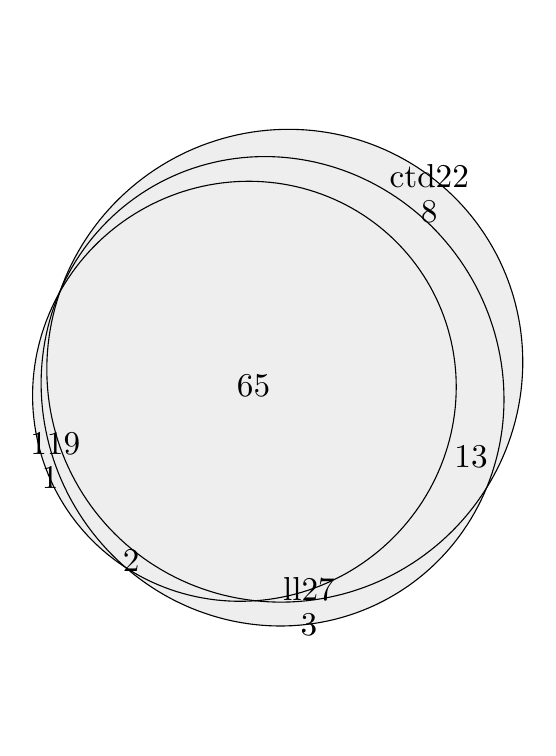
\begin{tikzpicture}[x=1pt,y=1pt]
\definecolor{fillColor}{RGB}{255,255,255}
\path[use as bounding box,fill=fillColor,fill opacity=0.00] (0,0) rectangle (180.67,252.94);
\begin{scope}
\path[clip] (  0.00,  0.00) rectangle (180.67,252.94);
\definecolor{fillColor}{RGB}{238,238,238}

\path[fill=fillColor,nonzero rule]
	( 34.24, 58.89) --
	( 32.25, 60.72) --
	( 30.33, 62.62) --
	( 28.46, 64.58) --
	( 26.65, 66.59) --
	( 24.91, 68.65) --
	( 23.22, 70.77) --
	( 21.60, 72.94) --
	( 20.05, 75.16) --
	( 18.57, 77.43) --
	( 17.16, 79.73) --
	( 15.81, 82.08) --
	( 14.54, 84.47) --
	( 13.35, 86.90) --
	( 12.22, 89.36) --
	( 11.18, 91.85) --
	( 10.21, 94.38) --
	(  9.32, 96.93) --
	(  8.51, 99.50) --
	(  7.78,102.10) --
	(  7.13,104.71) --
	(  6.56,107.35) --
	(  6.07,109.99) --
	(  5.66,112.65) --
	(  5.34,115.32) --
	(  5.10,117.99) --
	(  4.94,120.67) --
	(  4.86,123.35) --
	(  4.87,126.02) --
	(  4.96,128.69) --
	(  5.14,131.36) --
	(  5.40,134.01) --
	(  5.74,136.66) --
	(  6.16,139.28) --
	(  6.67,141.89) --
	(  7.26,144.48) --
	(  7.93,147.05) --
	(  8.67,149.59) --
	(  9.50,152.10) --
	( 10.41,154.58) --
	( 11.36,156.95) --
	( 10.81,155.96) --
	(  9.71,153.81) --
	(  8.67,151.62) --
	(  7.70,149.41) --
	(  6.80,147.16) --
	(  5.98,144.90) --
	(  5.22,142.61) --
	(  4.54,140.29) --
	(  3.94,137.96) --
	(  3.40,135.61) --
	(  2.94,133.25) --
	(  2.56,130.88) --
	(  2.25,128.50) --
	(  2.02,126.11) --
	(  1.86,123.72) --
	(  1.78,121.32) --
	(  1.78,118.92) --
	(  1.85,116.53) --
	(  2.00,114.14) --
	(  2.23,111.76) --
	(  2.53,109.39) --
	(  2.90,107.03) --
	(  3.35,104.69) --
	(  3.88,102.36) --
	(  4.48,100.05) --
	(  5.15, 97.77) --
	(  5.90, 95.50) --
	(  6.72, 93.27) --
	(  7.61, 91.06) --
	(  8.57, 88.88) --
	(  9.60, 86.73) --
	( 10.70, 84.62) --
	( 11.87, 82.55) --
	( 13.10, 80.51) --
	( 14.40, 78.52) --
	( 15.76, 76.56) --
	( 17.18, 74.66) --
	( 18.67, 72.80) --
	( 20.21, 70.99) --
	( 21.81, 69.22) --
	( 23.47, 67.52) --
	( 25.19, 65.86) --
	( 26.95, 64.26) --
	( 28.77, 62.72) --
	( 30.64, 61.23) --
	( 32.55, 59.81) --
	( 34.51, 58.45) --
	( 35.43, 57.85) --
	cycle;

\path[fill=fillColor,nonzero rule]
	( 11.67,157.51) --
	( 11.98,158.36) --
	( 11.39,157.03) --
	( 11.36,156.95) --
	cycle
	( 92.83, 36.75) --
	( 95.46, 36.84) --
	( 98.09, 37.02) --
	(100.71, 37.28) --
	(103.31, 37.62) --
	(105.90, 38.05) --
	(108.48, 38.56) --
	(111.03, 39.15) --
	(113.56, 39.83) --
	(116.07, 40.59) --
	(118.55, 41.42) --
	(120.99, 42.34) --
	(123.41, 43.34) --
	(125.79, 44.41) --
	(128.14, 45.56) --
	(130.44, 46.79) --
	(132.70, 48.09) --
	(134.92, 49.47) --
	(137.10, 50.91) --
	(139.22, 52.43) --
	(141.29, 54.02) --
	(143.31, 55.67) --
	(145.28, 57.39) --
	(147.19, 59.17) --
	(149.04, 61.02) --
	(150.83, 62.92) --
	(152.56, 64.89) --
	(154.22, 66.91) --
	(155.82, 68.98) --
	(157.36, 71.11) --
	(158.82, 73.29) --
	(160.21, 75.51) --
	(161.53, 77.79) --
	(162.78, 80.10) --
	(163.96, 82.46) --
	(165.06, 84.85) --
	(165.80, 86.62) --
	(165.48, 86.09) --
	(163.98, 83.81) --
	(162.42, 81.58) --
	(160.79, 79.40) --
	(159.09, 77.28) --
	(157.32, 75.20) --
	(155.49, 73.18) --
	(153.60, 71.22) --
	(151.64, 69.31) --
	(149.63, 67.47) --
	(147.56, 65.69) --
	(145.44, 63.98) --
	(143.26, 62.33) --
	(141.04, 60.75) --
	(138.76, 59.24) --
	(136.44, 57.80) --
	(134.08, 56.44) --
	(131.68, 55.15) --
	(129.23, 53.93) --
	(126.76, 52.79) --
	(124.24, 51.73) --
	(121.70, 50.75) --
	(119.13, 49.85) --
	(116.53, 49.02) --
	(113.91, 48.28) --
	(111.26, 47.63) --
	(108.60, 47.05) --
	(105.92, 46.56) --
	(103.23, 46.15) --
	(100.53, 45.83) --
	( 97.83, 45.59) --
	( 95.11, 45.43) --
	( 92.40, 45.36) --
	( 89.68, 45.38) --
	( 86.97, 45.48) --
	( 84.27, 45.67) --
	( 82.32, 45.86) --
	( 80.01, 45.73) --
	( 77.60, 45.66) --
	( 75.18, 45.68) --
	( 72.77, 45.76) --
	( 70.36, 45.93) --
	( 67.96, 46.16) --
	( 65.57, 46.48) --
	( 63.20, 46.87) --
	( 60.83, 47.33) --
	( 58.49, 47.87) --
	( 56.17, 48.48) --
	( 53.86, 49.16) --
	( 51.59, 49.91) --
	( 49.34, 50.74) --
	( 47.11, 51.64) --
	( 44.92, 52.60) --
	( 42.76, 53.64) --
	( 40.64, 54.74) --
	( 38.56, 55.91) --
	( 36.51, 57.15) --
	( 35.43, 57.85) --
	( 36.27, 57.12) --
	( 38.36, 55.41) --
	( 40.50, 53.76) --
	( 42.69, 52.19) --
	( 44.92, 50.68) --
	( 47.19, 49.25) --
	( 49.51, 47.88) --
	( 51.86, 46.59) --
	( 54.26, 45.38) --
	( 56.68, 44.24) --
	( 59.14, 43.18) --
	( 61.63, 42.19) --
	( 64.14, 41.29) --
	( 66.68, 40.46) --
	( 69.24, 39.72) --
	( 71.82, 39.05) --
	( 74.41, 38.47) --
	( 77.02, 37.98) --
	( 79.64, 37.56) --
	( 82.27, 37.23) --
	( 84.91, 36.98) --
	( 87.55, 36.82) --
	( 90.19, 36.74) --
	cycle;

\path[fill=fillColor,nonzero rule]
	(166.90, 88.41) --
	(168.24, 90.77) --
	(169.51, 93.17) --
	(170.71, 95.61) --
	(171.83, 98.09) --
	(172.87,100.60) --
	(173.83,103.14) --
	(174.70,105.70) --
	(175.50,108.29) --
	(176.22,110.90) --
	(176.85,113.54) --
	(177.40,116.19) --
	(177.86,118.85) --
	(178.24,121.53) --
	(178.53,124.21) --
	(178.74,126.90) --
	(178.87,129.60) --
	(178.90,132.30) --
	(178.86,134.99) --
	(178.72,137.68) --
	(178.50,140.37) --
	(178.20,143.04) --
	(177.81,145.71) --
	(177.33,148.35) --
	(176.77,150.98) --
	(176.13,153.60) --
	(175.41,156.18) --
	(174.60,158.74) --
	(173.71,161.28) --
	(172.74,163.78) --
	(171.69,166.25) --
	(170.57,168.69) --
	(169.36,171.09) --
	(168.08,173.44) --
	(166.72,175.76) --
	(165.29,178.03) --
	(163.79,180.25) --
	(162.22,182.43) --
	(160.58,184.55) --
	(158.87,186.62) --
	(157.10,188.63) --
	(155.26,190.59) --
	(153.36,192.48) --
	(151.40,194.32) --
	(149.38,196.09) --
	(147.30,197.79) --
	(145.17,199.43) --
	(142.99,201.00) --
	(140.76,202.51) --
	(138.48,203.93) --
	(136.15,205.29) --
	(133.78,206.57) --
	(131.38,207.78) --
	(128.93,208.91) --
	(126.45,209.96) --
	(123.93,210.93) --
	(121.38,211.83) --
	(118.81,212.64) --
	(116.20,213.37) --
	(113.58,214.02) --
	(110.93,214.58) --
	(108.27,215.07) --
	(105.59,215.46) --
	(102.90,215.78) --
	(100.20,216.01) --
	( 97.49,216.15) --
	( 94.78,216.21) --
	( 92.06,216.18) --
	( 89.35,216.07) --
	( 86.64,215.87) --
	( 83.93,215.59) --
	( 81.24,215.23) --
	( 78.55,214.78) --
	( 75.88,214.24) --
	( 73.23,213.62) --
	( 70.60,212.92) --
	( 67.99,212.14) --
	( 65.40,211.28) --
	( 62.84,210.34) --
	( 60.32,209.32) --
	( 57.82,208.22) --
	( 55.36,207.04) --
	( 52.94,205.78) --
	( 50.55,204.46) --
	( 48.21,203.05) --
	( 45.91,201.58) --
	( 43.66,200.04) --
	( 41.46,198.42) --
	( 39.31,196.74) --
	( 37.22,194.99) --
	( 35.18,193.18) --
	( 33.19,191.31) --
	( 31.27,189.38) --
	( 29.41,187.39) --
	( 27.61,185.34) --
	( 25.87,183.24) --
	( 24.21,181.08) --
	( 22.61,178.88) --
	( 21.08,176.62) --
	( 19.62,174.32) --
	( 18.24,171.98) --
	( 16.93,169.60) --
	( 15.70,167.18) --
	( 14.54,164.72) --
	( 13.46,162.23) --
	( 12.46,159.71) --
	( 11.98,158.36) --
	( 12.46,159.45) --
	( 13.59,161.82) --
	( 14.81,164.16) --
	( 16.09,166.45) --
	( 17.45,168.70) --
	( 18.88,170.90) --
	( 20.38,173.06) --
	( 21.94,175.16) --
	( 23.57,177.21) --
	( 25.27,179.20) --
	( 27.03,181.13) --
	( 28.85,183.01) --
	( 30.73,184.82) --
	( 32.67,186.58) --
	( 34.66,188.26) --
	( 36.71,189.88) --
	( 38.81,191.43) --
	( 40.96,192.92) --
	( 43.16,194.33) --
	( 45.40,195.67) --
	( 47.68,196.93) --
	( 50.01,198.12) --
	( 52.37,199.23) --
	( 54.77,200.27) --
	( 57.20,201.23) --
	( 59.66,202.10) --
	( 62.16,202.90) --
	( 64.68,203.62) --
	( 67.22,204.25) --
	( 69.78,204.81) --
	( 72.36,205.27) --
	( 74.96,205.66) --
	( 77.58,205.96) --
	( 80.20,206.18) --
	( 82.83,206.31) --
	( 85.47,206.36) --
	( 88.11,206.33) --
	( 90.75,206.21) --
	( 93.38,206.00) --
	( 96.02,205.71) --
	( 98.64,205.34) --
	(101.26,204.88) --
	(103.86,204.35) --
	(106.45,203.72) --
	(109.02,203.02) --
	(111.57,202.24) --
	(114.09,201.37) --
	(116.59,200.43) --
	(119.07,199.40) --
	(121.51,198.30) --
	(123.92,197.12) --
	(126.29,195.87) --
	(128.63,194.54) --
	(130.92,193.14) --
	(133.18,191.67) --
	(135.39,190.13) --
	(137.55,188.52) --
	(139.66,186.85) --
	(141.73,185.10) --
	(143.73,183.30) --
	(145.69,181.43) --
	(147.59,179.51) --
	(149.43,177.52) --
	(151.20,175.48) --
	(152.92,173.39) --
	(154.57,171.25) --
	(156.15,169.05) --
	(157.67,166.81) --
	(159.12,164.52) --
	(160.50,162.19) --
	(161.81,159.82) --
	(163.04,157.42) --
	(164.20,154.97) --
	(165.28,152.49) --
	(166.29,149.99) --
	(167.22,147.45) --
	(168.07,144.89) --
	(168.84,142.30) --
	(169.53,139.69) --
	(170.14,137.07) --
	(170.67,134.43) --
	(171.12,131.78) --
	(171.49,129.11) --
	(171.77,126.44) --
	(171.97,123.77) --
	(172.08,121.09) --
	(172.12,118.41) --
	(172.07,115.74) --
	(171.93,113.07) --
	(171.72,110.41) --
	(171.42,107.76) --
	(171.03,105.13) --
	(170.57,102.51) --
	(170.02, 99.91) --
	(169.39, 97.33) --
	(168.68, 94.78) --
	(167.90, 92.25) --
	(167.03, 89.75) --
	(166.08, 87.29) --
	(165.80, 86.62) --
	cycle;

\path[fill=fillColor,nonzero rule]
	( 80.01, 45.73) --
	( 82.32, 45.86) --
	( 81.57, 45.94) --
	( 78.89, 46.29) --
	( 76.22, 46.73) --
	( 73.56, 47.26) --
	( 70.92, 47.86) --
	( 68.31, 48.55) --
	( 65.72, 49.33) --
	( 63.16, 50.18) --
	( 60.63, 51.11) --
	( 58.13, 52.12) --
	( 55.66, 53.21) --
	( 53.23, 54.38) --
	( 50.85, 55.63) --
	( 48.50, 56.95) --
	( 46.20, 58.34) --
	( 43.94, 59.80) --
	( 41.73, 61.34) --
	( 39.58, 62.95) --
	( 37.47, 64.62) --
	( 35.43, 66.36) --
	( 33.44, 68.16) --
	( 31.50, 70.03) --
	( 29.63, 71.95) --
	( 27.83, 73.94) --
	( 26.09, 75.98) --
	( 24.41, 78.07) --
	( 22.80, 80.22) --
	( 21.27, 82.42) --
	( 19.80, 84.67) --
	( 18.41, 86.96) --
	( 17.09, 89.30) --
	( 15.85, 91.68) --
	( 14.68, 94.09) --
	( 13.59, 96.55) --
	( 12.58, 99.03) --
	( 11.65,101.55) --
	( 10.81,104.10) --
	( 10.04,106.68) --
	(  9.36,109.28) --
	(  8.75,111.90) --
	(  8.24,114.54) --
	(  7.81,117.19) --
	(  7.46,119.86) --
	(  7.20,122.54) --
	(  7.02,125.23) --
	(  6.93,127.92) --
	(  6.92,130.62) --
	(  7.00,133.32) --
	(  7.17,136.01) --
	(  7.42,138.70) --
	(  7.76,141.38) --
	(  8.18,144.05) --
	(  8.69,146.71) --
	(  9.28,149.35) --
	(  9.95,151.97) --
	( 10.71,154.58) --
	( 11.54,157.15) --
	( 11.67,157.51) --
	( 11.36,156.95) --
	( 10.41,154.58) --
	(  9.50,152.10) --
	(  8.67,149.59) --
	(  7.93,147.05) --
	(  7.26,144.48) --
	(  6.67,141.89) --
	(  6.16,139.28) --
	(  5.74,136.66) --
	(  5.40,134.01) --
	(  5.14,131.36) --
	(  4.96,128.69) --
	(  4.87,126.02) --
	(  4.86,123.35) --
	(  4.94,120.67) --
	(  5.10,117.99) --
	(  5.34,115.32) --
	(  5.66,112.65) --
	(  6.07,109.99) --
	(  6.56,107.35) --
	(  7.13,104.71) --
	(  7.78,102.10) --
	(  8.51, 99.50) --
	(  9.32, 96.93) --
	( 10.21, 94.38) --
	( 11.18, 91.85) --
	( 12.22, 89.36) --
	( 13.35, 86.90) --
	( 14.54, 84.47) --
	( 15.81, 82.08) --
	( 17.16, 79.73) --
	( 18.57, 77.43) --
	( 20.05, 75.16) --
	( 21.60, 72.94) --
	( 23.22, 70.77) --
	( 24.91, 68.65) --
	( 26.65, 66.59) --
	( 28.46, 64.58) --
	( 30.33, 62.62) --
	( 32.25, 60.72) --
	( 34.24, 58.89) --
	( 35.43, 57.85) --
	( 36.51, 57.15) --
	( 38.56, 55.91) --
	( 40.64, 54.74) --
	( 42.76, 53.64) --
	( 44.92, 52.60) --
	( 47.11, 51.64) --
	( 49.34, 50.74) --
	( 51.59, 49.91) --
	( 53.86, 49.16) --
	( 56.17, 48.48) --
	( 58.49, 47.87) --
	( 60.83, 47.33) --
	( 63.20, 46.87) --
	( 65.57, 46.48) --
	( 67.96, 46.16) --
	( 70.36, 45.93) --
	( 72.77, 45.76) --
	( 75.18, 45.68) --
	( 77.60, 45.66) --
	cycle;

\path[fill=fillColor,nonzero rule]
	( 95.11, 45.43) --
	( 97.83, 45.59) --
	(100.53, 45.83) --
	(103.23, 46.15) --
	(105.92, 46.56) --
	(108.60, 47.05) --
	(111.26, 47.63) --
	(113.91, 48.28) --
	(116.53, 49.02) --
	(119.13, 49.85) --
	(121.70, 50.75) --
	(124.24, 51.73) --
	(126.76, 52.79) --
	(129.23, 53.93) --
	(131.68, 55.15) --
	(134.08, 56.44) --
	(136.44, 57.80) --
	(138.76, 59.24) --
	(141.04, 60.75) --
	(143.26, 62.33) --
	(145.44, 63.98) --
	(147.56, 65.69) --
	(149.63, 67.47) --
	(151.64, 69.31) --
	(153.60, 71.22) --
	(155.49, 73.18) --
	(157.32, 75.20) --
	(159.09, 77.28) --
	(160.79, 79.40) --
	(162.42, 81.58) --
	(163.98, 83.81) --
	(165.48, 86.09) --
	(165.80, 86.62) --
	(166.08, 87.29) --
	(167.03, 89.75) --
	(167.90, 92.25) --
	(168.68, 94.78) --
	(169.39, 97.33) --
	(170.02, 99.91) --
	(170.57,102.51) --
	(171.03,105.13) --
	(171.42,107.76) --
	(171.72,110.41) --
	(171.93,113.07) --
	(172.07,115.74) --
	(172.12,118.41) --
	(172.08,121.09) --
	(171.97,123.77) --
	(171.77,126.44) --
	(171.49,129.11) --
	(171.12,131.78) --
	(170.67,134.43) --
	(170.14,137.07) --
	(169.53,139.69) --
	(168.84,142.30) --
	(168.07,144.89) --
	(167.22,147.45) --
	(166.29,149.99) --
	(165.28,152.49) --
	(164.20,154.97) --
	(163.04,157.42) --
	(161.81,159.82) --
	(160.50,162.19) --
	(159.12,164.52) --
	(157.67,166.81) --
	(156.15,169.05) --
	(154.57,171.25) --
	(152.92,173.39) --
	(151.20,175.48) --
	(149.43,177.52) --
	(147.59,179.51) --
	(145.69,181.43) --
	(143.73,183.30) --
	(141.73,185.10) --
	(139.66,186.85) --
	(137.55,188.52) --
	(135.39,190.13) --
	(133.18,191.67) --
	(130.92,193.14) --
	(128.63,194.54) --
	(126.29,195.87) --
	(123.92,197.12) --
	(121.51,198.30) --
	(119.07,199.40) --
	(116.59,200.43) --
	(114.09,201.37) --
	(111.57,202.24) --
	(109.02,203.02) --
	(106.45,203.72) --
	(103.86,204.35) --
	(101.26,204.88) --
	( 98.64,205.34) --
	( 96.02,205.71) --
	( 93.38,206.00) --
	( 90.75,206.21) --
	( 88.11,206.33) --
	( 85.47,206.36) --
	( 82.83,206.31) --
	( 80.20,206.18) --
	( 77.58,205.96) --
	( 74.96,205.66) --
	( 72.36,205.27) --
	( 69.78,204.81) --
	( 67.22,204.25) --
	( 64.68,203.62) --
	( 62.16,202.90) --
	( 59.66,202.10) --
	( 57.20,201.23) --
	( 54.77,200.27) --
	( 52.37,199.23) --
	( 50.01,198.12) --
	( 47.68,196.93) --
	( 45.40,195.67) --
	( 43.16,194.33) --
	( 40.96,192.92) --
	( 38.81,191.43) --
	( 36.71,189.88) --
	( 34.66,188.26) --
	( 32.67,186.58) --
	( 30.73,184.82) --
	( 28.85,183.01) --
	( 27.03,181.13) --
	( 25.27,179.20) --
	( 23.57,177.21) --
	( 21.94,175.16) --
	( 20.38,173.06) --
	( 18.88,170.90) --
	( 17.45,168.70) --
	( 16.09,166.45) --
	( 14.81,164.16) --
	( 13.59,161.82) --
	( 12.46,159.45) --
	( 11.98,158.36) --
	( 11.67,157.51) --
	( 11.98,158.08) --
	( 13.22,160.16) --
	( 14.53,162.20) --
	( 15.89,164.20) --
	( 17.32,166.16) --
	( 18.81,168.08) --
	( 20.36,169.95) --
	( 21.97,171.77) --
	( 23.64,173.54) --
	( 25.35,175.26) --
	( 27.13,176.93) --
	( 28.95,178.54) --
	( 30.82,180.09) --
	( 32.74,181.59) --
	( 34.70,183.02) --
	( 36.71,184.40) --
	( 38.76,185.71) --
	( 40.85,186.95) --
	( 42.97,188.14) --
	( 45.13,189.25) --
	( 47.33,190.30) --
	( 49.55,191.28) --
	( 51.81,192.19) --
	( 54.09,193.03) --
	( 56.39,193.80) --
	( 58.72,194.50) --
	( 61.06,195.12) --
	( 63.42,195.67) --
	( 65.80,196.15) --
	( 68.19,196.55) --
	( 70.59,196.88) --
	( 73.00,197.13) --
	( 75.41,197.31) --
	( 77.83,197.41) --
	( 80.25,197.44) --
	( 82.66,197.39) --
	( 85.07,197.26) --
	( 87.48,197.06) --
	( 89.87,196.79) --
	( 92.25,196.44) --
	( 94.62,196.01) --
	( 96.98,195.51) --
	( 99.31,194.94) --
	(101.62,194.29) --
	(103.91,193.57) --
	(106.18,192.78) --
	(108.41,191.92) --
	(110.62,190.99) --
	(112.80,189.98) --
	(114.94,188.92) --
	(117.04,187.78) --
	(119.11,186.58) --
	(121.13,185.31) --
	(123.11,183.98) --
	(125.05,182.58) --
	(126.94,181.13) --
	(128.78,179.62) --
	(130.57,178.05) --
	(132.31,176.42) --
	(134.00,174.73) --
	(135.63,173.00) --
	(137.20,171.21) --
	(138.72,169.38) --
	(140.17,167.49) --
	(141.56,165.56) --
	(142.89,163.59) --
	(144.16,161.57) --
	(145.36,159.52) --
	(146.49,157.43) --
	(147.56,155.30) --
	(148.55,153.13) --
	(149.48,150.94) --
	(150.33,148.72) --
	(151.12,146.47) --
	(151.83,144.19) --
	(152.46,141.89) --
	(153.03,139.57) --
	(153.52,137.24) --
	(153.93,134.89) --
	(154.27,132.52) --
	(154.53,130.15) --
	(154.72,127.76) --
	(154.83,125.37) --
	(154.86,122.98) --
	(154.82,120.58) --
	(154.70,118.18) --
	(154.51,115.79) --
	(154.24,113.41) --
	(153.89,111.03) --
	(153.47,108.66) --
	(152.98,106.31) --
	(152.41,103.97) --
	(151.76,101.65) --
	(151.04, 99.34) --
	(150.25, 97.06) --
	(149.39, 94.81) --
	(148.46, 92.58) --
	(147.46, 90.38) --
	(146.38, 88.21) --
	(145.25, 86.08) --
	(144.04, 83.98) --
	(142.77, 81.91) --
	(141.43, 79.89) --
	(140.03, 77.91) --
	(138.57, 75.97) --
	(137.05, 74.08) --
	(135.47, 72.23) --
	(133.84, 70.44) --
	(132.15, 68.69) --
	(130.40, 67.00) --
	(128.60, 65.36) --
	(126.76, 63.78) --
	(124.86, 62.25) --
	(122.92, 60.79) --
	(120.94, 59.38) --
	(118.91, 58.04) --
	(116.84, 56.76) --
	(114.73, 55.54) --
	(112.59, 54.40) --
	(110.41, 53.31) --
	(108.20, 52.30) --
	(105.96, 51.35) --
	(103.69, 50.48) --
	(101.40, 49.67) --
	( 99.08, 48.94) --
	( 96.75, 48.28) --
	( 94.39, 47.69) --
	( 92.02, 47.18) --
	( 89.64, 46.74) --
	( 87.24, 46.37) --
	( 84.84, 46.08) --
	( 82.43, 45.87) --
	( 82.32, 45.86) --
	( 84.27, 45.67) --
	( 86.97, 45.48) --
	( 89.68, 45.38) --
	( 92.40, 45.36) --
	cycle;

\path[fill=fillColor,nonzero rule]
	( 82.43, 45.87) --
	( 84.84, 46.08) --
	( 87.24, 46.37) --
	( 89.64, 46.74) --
	( 92.02, 47.18) --
	( 94.39, 47.69) --
	( 96.75, 48.28) --
	( 99.08, 48.94) --
	(101.40, 49.67) --
	(103.69, 50.48) --
	(105.96, 51.35) --
	(108.20, 52.30) --
	(110.41, 53.31) --
	(112.59, 54.40) --
	(114.73, 55.54) --
	(116.84, 56.76) --
	(118.91, 58.04) --
	(120.94, 59.38) --
	(122.92, 60.79) --
	(124.86, 62.25) --
	(126.76, 63.78) --
	(128.60, 65.36) --
	(130.40, 67.00) --
	(132.15, 68.69) --
	(133.84, 70.44) --
	(135.47, 72.23) --
	(137.05, 74.08) --
	(138.57, 75.97) --
	(140.03, 77.91) --
	(141.43, 79.89) --
	(142.77, 81.91) --
	(144.04, 83.98) --
	(145.25, 86.08) --
	(146.38, 88.21) --
	(147.46, 90.38) --
	(148.46, 92.58) --
	(149.39, 94.81) --
	(150.25, 97.06) --
	(151.04, 99.34) --
	(151.76,101.65) --
	(152.41,103.97) --
	(152.98,106.31) --
	(153.47,108.66) --
	(153.89,111.03) --
	(154.24,113.41) --
	(154.51,115.79) --
	(154.70,118.18) --
	(154.82,120.58) --
	(154.86,122.98) --
	(154.83,125.37) --
	(154.72,127.76) --
	(154.53,130.15) --
	(154.27,132.52) --
	(153.93,134.89) --
	(153.52,137.24) --
	(153.03,139.57) --
	(152.46,141.89) --
	(151.83,144.19) --
	(151.12,146.47) --
	(150.33,148.72) --
	(149.48,150.94) --
	(148.55,153.13) --
	(147.56,155.30) --
	(146.49,157.43) --
	(145.36,159.52) --
	(144.16,161.57) --
	(142.89,163.59) --
	(141.56,165.56) --
	(140.17,167.49) --
	(138.72,169.38) --
	(137.20,171.21) --
	(135.63,173.00) --
	(134.00,174.73) --
	(132.31,176.42) --
	(130.57,178.05) --
	(128.78,179.62) --
	(126.94,181.13) --
	(125.05,182.58) --
	(123.11,183.98) --
	(121.13,185.31) --
	(119.11,186.58) --
	(117.04,187.78) --
	(114.94,188.92) --
	(112.80,189.98) --
	(110.62,190.99) --
	(108.41,191.92) --
	(106.18,192.78) --
	(103.91,193.57) --
	(101.62,194.29) --
	( 99.31,194.94) --
	( 96.98,195.51) --
	( 94.62,196.01) --
	( 92.25,196.44) --
	( 89.87,196.79) --
	( 87.48,197.06) --
	( 85.07,197.26) --
	( 82.66,197.39) --
	( 80.25,197.44) --
	( 77.83,197.41) --
	( 75.41,197.31) --
	( 73.00,197.13) --
	( 70.59,196.88) --
	( 68.19,196.55) --
	( 65.80,196.15) --
	( 63.42,195.67) --
	( 61.06,195.12) --
	( 58.72,194.50) --
	( 56.39,193.80) --
	( 54.09,193.03) --
	( 51.81,192.19) --
	( 49.55,191.28) --
	( 47.33,190.30) --
	( 45.13,189.25) --
	( 42.97,188.14) --
	( 40.85,186.95) --
	( 38.76,185.71) --
	( 36.71,184.40) --
	( 34.70,183.02) --
	( 32.74,181.59) --
	( 30.82,180.09) --
	( 28.95,178.54) --
	( 27.13,176.93) --
	( 25.35,175.26) --
	( 23.64,173.54) --
	( 21.97,171.77) --
	( 20.36,169.95) --
	( 18.81,168.08) --
	( 17.32,166.16) --
	( 15.89,164.20) --
	( 14.53,162.20) --
	( 13.22,160.16) --
	( 11.98,158.08) --
	( 11.67,157.51) --
	( 11.54,157.15) --
	( 10.71,154.58) --
	(  9.95,151.97) --
	(  9.28,149.35) --
	(  8.69,146.71) --
	(  8.18,144.05) --
	(  7.76,141.38) --
	(  7.42,138.70) --
	(  7.17,136.01) --
	(  7.00,133.32) --
	(  6.92,130.62) --
	(  6.93,127.92) --
	(  7.02,125.23) --
	(  7.20,122.54) --
	(  7.46,119.86) --
	(  7.81,117.19) --
	(  8.24,114.54) --
	(  8.75,111.90) --
	(  9.36,109.28) --
	( 10.04,106.68) --
	( 10.81,104.10) --
	( 11.65,101.55) --
	( 12.58, 99.03) --
	( 13.59, 96.55) --
	( 14.68, 94.09) --
	( 15.85, 91.68) --
	( 17.09, 89.30) --
	( 18.41, 86.96) --
	( 19.80, 84.67) --
	( 21.27, 82.42) --
	( 22.80, 80.22) --
	( 24.41, 78.07) --
	( 26.09, 75.98) --
	( 27.83, 73.94) --
	( 29.63, 71.95) --
	( 31.50, 70.03) --
	( 33.44, 68.16) --
	( 35.43, 66.36) --
	( 37.47, 64.62) --
	( 39.58, 62.95) --
	( 41.73, 61.34) --
	( 43.94, 59.80) --
	( 46.20, 58.34) --
	( 48.50, 56.95) --
	( 50.85, 55.63) --
	( 53.23, 54.38) --
	( 55.66, 53.21) --
	( 58.13, 52.12) --
	( 60.63, 51.11) --
	( 63.16, 50.18) --
	( 65.72, 49.33) --
	( 68.31, 48.55) --
	( 70.92, 47.86) --
	( 73.56, 47.26) --
	( 76.22, 46.73) --
	( 78.89, 46.29) --
	( 81.57, 45.94) --
	( 82.32, 45.86) --
	cycle;
\definecolor{drawColor}{RGB}{0,0,0}

\path[draw=drawColor,line width= 0.4pt,line join=round,line cap=round] ( 36.71,184.40) --
	( 34.70,183.02) --
	( 32.74,181.59) --
	( 30.82,180.09) --
	( 28.95,178.54) --
	( 27.13,176.93) --
	( 25.35,175.26) --
	( 23.64,173.54) --
	( 21.97,171.77) --
	( 20.36,169.95) --
	( 18.81,168.08) --
	( 17.32,166.16) --
	( 15.89,164.20) --
	( 14.53,162.20) --
	( 13.22,160.16) --
	( 11.98,158.08) --
	( 10.81,155.96) --
	(  9.71,153.81) --
	(  8.67,151.62) --
	(  7.70,149.41) --
	(  6.80,147.16) --
	(  5.98,144.90) --
	(  5.22,142.61) --
	(  4.54,140.29) --
	(  3.94,137.96) --
	(  3.40,135.61) --
	(  2.94,133.25) --
	(  2.56,130.88) --
	(  2.25,128.50) --
	(  2.02,126.11) --
	(  1.86,123.72) --
	(  1.78,121.32) --
	(  1.78,118.92) --
	(  1.85,116.53) --
	(  2.00,114.14) --
	(  2.23,111.76) --
	(  2.53,109.39) --
	(  2.90,107.03) --
	(  3.35,104.69) --
	(  3.88,102.36) --
	(  4.48,100.05) --
	(  5.15, 97.77) --
	(  5.90, 95.50) --
	(  6.72, 93.27) --
	(  7.61, 91.06) --
	(  8.57, 88.88) --
	(  9.60, 86.73) --
	( 10.70, 84.62) --
	( 11.87, 82.55) --
	( 13.10, 80.51) --
	( 14.40, 78.52) --
	( 15.76, 76.56) --
	( 17.18, 74.66) --
	( 18.67, 72.80) --
	( 20.21, 70.99) --
	( 21.81, 69.22) --
	( 23.47, 67.52) --
	( 25.19, 65.86) --
	( 26.95, 64.26) --
	( 28.77, 62.72) --
	( 30.64, 61.23) --
	( 32.55, 59.81) --
	( 34.51, 58.45) --
	( 36.51, 57.15) --
	( 38.56, 55.91) --
	( 40.64, 54.74) --
	( 42.76, 53.64) --
	( 44.92, 52.60) --
	( 47.11, 51.64) --
	( 49.34, 50.74) --
	( 51.59, 49.91) --
	( 53.86, 49.16) --
	( 56.17, 48.48) --
	( 58.49, 47.87) --
	( 60.83, 47.33) --
	( 63.20, 46.87) --
	( 65.57, 46.48) --
	( 67.96, 46.16) --
	( 70.36, 45.93) --
	( 72.77, 45.76) --
	( 75.18, 45.68) --
	( 77.60, 45.66) --
	( 80.01, 45.73) --
	( 82.43, 45.87) --
	( 84.84, 46.08) --
	( 87.24, 46.37) --
	( 89.64, 46.74) --
	( 92.02, 47.18) --
	( 94.39, 47.69) --
	( 96.75, 48.28) --
	( 99.08, 48.94) --
	(101.40, 49.67) --
	(103.69, 50.48) --
	(105.96, 51.35) --
	(108.20, 52.30) --
	(110.41, 53.31) --
	(112.59, 54.40) --
	(114.73, 55.54) --
	(116.84, 56.76) --
	(118.91, 58.04) --
	(120.94, 59.38) --
	(122.92, 60.79) --
	(124.86, 62.25) --
	(126.76, 63.78) --
	(128.60, 65.36) --
	(130.40, 67.00) --
	(132.15, 68.69) --
	(133.84, 70.44) --
	(135.47, 72.23) --
	(137.05, 74.08) --
	(138.57, 75.97) --
	(140.03, 77.91) --
	(141.43, 79.89) --
	(142.77, 81.91) --
	(144.04, 83.98) --
	(145.25, 86.08) --
	(146.38, 88.21) --
	(147.46, 90.38) --
	(148.46, 92.58) --
	(149.39, 94.81) --
	(150.25, 97.06) --
	(151.04, 99.34) --
	(151.76,101.65) --
	(152.41,103.97) --
	(152.98,106.31) --
	(153.47,108.66) --
	(153.89,111.03) --
	(154.24,113.41) --
	(154.51,115.79) --
	(154.70,118.18) --
	(154.82,120.58) --
	(154.86,122.98) --
	(154.83,125.37) --
	(154.72,127.76) --
	(154.53,130.15) --
	(154.27,132.52) --
	(153.93,134.89) --
	(153.52,137.24) --
	(153.03,139.57) --
	(152.46,141.89) --
	(151.83,144.19) --
	(151.12,146.47) --
	(150.33,148.72) --
	(149.48,150.94) --
	(148.55,153.13) --
	(147.56,155.30) --
	(146.49,157.43) --
	(145.36,159.52) --
	(144.16,161.57) --
	(142.89,163.59) --
	(141.56,165.56) --
	(140.17,167.49) --
	(138.72,169.38) --
	(137.20,171.21) --
	(135.63,173.00) --
	(134.00,174.73) --
	(132.31,176.42) --
	(130.57,178.05) --
	(128.78,179.62) --
	(126.94,181.13) --
	(125.05,182.58) --
	(123.11,183.98) --
	(121.13,185.31) --
	(119.11,186.58) --
	(117.04,187.78) --
	(114.94,188.92) --
	(112.80,189.98) --
	(110.62,190.99) --
	(108.41,191.92) --
	(106.18,192.78) --
	(103.91,193.57) --
	(101.62,194.29) --
	( 99.31,194.94) --
	( 96.98,195.51) --
	( 94.62,196.01) --
	( 92.25,196.44) --
	( 89.87,196.79) --
	( 87.48,197.06) --
	( 85.07,197.26) --
	( 82.66,197.39) --
	( 80.25,197.44) --
	( 77.83,197.41) --
	( 75.41,197.31) --
	( 73.00,197.13) --
	( 70.59,196.88) --
	( 68.19,196.55) --
	( 65.80,196.15) --
	( 63.42,195.67) --
	( 61.06,195.12) --
	( 58.72,194.50) --
	( 56.39,193.80) --
	( 54.09,193.03) --
	( 51.81,192.19) --
	( 49.55,191.28) --
	( 47.33,190.30) --
	( 45.13,189.25) --
	( 42.97,188.14) --
	( 40.85,186.95) --
	( 38.76,185.71) --
	( 36.71,184.40);

\path[draw=drawColor,line width= 0.4pt,line join=round,line cap=round] ( 40.96,192.92) --
	( 38.81,191.43) --
	( 36.71,189.88) --
	( 34.66,188.26) --
	( 32.67,186.58) --
	( 30.73,184.82) --
	( 28.85,183.01) --
	( 27.03,181.13) --
	( 25.27,179.20) --
	( 23.57,177.21) --
	( 21.94,175.16) --
	( 20.38,173.06) --
	( 18.88,170.90) --
	( 17.45,168.70) --
	( 16.09,166.45) --
	( 14.81,164.16) --
	( 13.59,161.82) --
	( 12.46,159.45) --
	( 11.39,157.03) --
	( 10.41,154.58) --
	(  9.50,152.10) --
	(  8.67,149.59) --
	(  7.93,147.05) --
	(  7.26,144.48) --
	(  6.67,141.89) --
	(  6.16,139.28) --
	(  5.74,136.66) --
	(  5.40,134.01) --
	(  5.14,131.36) --
	(  4.96,128.69) --
	(  4.87,126.02) --
	(  4.86,123.35) --
	(  4.94,120.67) --
	(  5.10,117.99) --
	(  5.34,115.32) --
	(  5.66,112.65) --
	(  6.07,109.99) --
	(  6.56,107.35) --
	(  7.13,104.71) --
	(  7.78,102.10) --
	(  8.51, 99.50) --
	(  9.32, 96.93) --
	( 10.21, 94.38) --
	( 11.18, 91.85) --
	( 12.22, 89.36) --
	( 13.35, 86.90) --
	( 14.54, 84.47) --
	( 15.81, 82.08) --
	( 17.16, 79.73) --
	( 18.57, 77.43) --
	( 20.05, 75.16) --
	( 21.60, 72.94) --
	( 23.22, 70.77) --
	( 24.91, 68.65) --
	( 26.65, 66.59) --
	( 28.46, 64.58) --
	( 30.33, 62.62) --
	( 32.25, 60.72) --
	( 34.24, 58.89) --
	( 36.27, 57.12) --
	( 38.36, 55.41) --
	( 40.50, 53.76) --
	( 42.69, 52.19) --
	( 44.92, 50.68) --
	( 47.19, 49.25) --
	( 49.51, 47.88) --
	( 51.86, 46.59) --
	( 54.26, 45.38) --
	( 56.68, 44.24) --
	( 59.14, 43.18) --
	( 61.63, 42.19) --
	( 64.14, 41.29) --
	( 66.68, 40.46) --
	( 69.24, 39.72) --
	( 71.82, 39.05) --
	( 74.41, 38.47) --
	( 77.02, 37.98) --
	( 79.64, 37.56) --
	( 82.27, 37.23) --
	( 84.91, 36.98) --
	( 87.55, 36.82) --
	( 90.19, 36.74) --
	( 92.83, 36.75) --
	( 95.46, 36.84) --
	( 98.09, 37.02) --
	(100.71, 37.28) --
	(103.31, 37.62) --
	(105.90, 38.05) --
	(108.48, 38.56) --
	(111.03, 39.15) --
	(113.56, 39.83) --
	(116.07, 40.59) --
	(118.55, 41.42) --
	(120.99, 42.34) --
	(123.41, 43.34) --
	(125.79, 44.41) --
	(128.14, 45.56) --
	(130.44, 46.79) --
	(132.70, 48.09) --
	(134.92, 49.47) --
	(137.10, 50.91) --
	(139.22, 52.43) --
	(141.29, 54.02) --
	(143.31, 55.67) --
	(145.28, 57.39) --
	(147.19, 59.17) --
	(149.04, 61.02) --
	(150.83, 62.92) --
	(152.56, 64.89) --
	(154.22, 66.91) --
	(155.82, 68.98) --
	(157.36, 71.11) --
	(158.82, 73.29) --
	(160.21, 75.51) --
	(161.53, 77.79) --
	(162.78, 80.10) --
	(163.96, 82.46) --
	(165.06, 84.85) --
	(166.08, 87.29) --
	(167.03, 89.75) --
	(167.90, 92.25) --
	(168.68, 94.78) --
	(169.39, 97.33) --
	(170.02, 99.91) --
	(170.57,102.51) --
	(171.03,105.13) --
	(171.42,107.76) --
	(171.72,110.41) --
	(171.93,113.07) --
	(172.07,115.74) --
	(172.12,118.41) --
	(172.08,121.09) --
	(171.97,123.77) --
	(171.77,126.44) --
	(171.49,129.11) --
	(171.12,131.78) --
	(170.67,134.43) --
	(170.14,137.07) --
	(169.53,139.69) --
	(168.84,142.30) --
	(168.07,144.89) --
	(167.22,147.45) --
	(166.29,149.99) --
	(165.28,152.49) --
	(164.20,154.97) --
	(163.04,157.42) --
	(161.81,159.82) --
	(160.50,162.19) --
	(159.12,164.52) --
	(157.67,166.81) --
	(156.15,169.05) --
	(154.57,171.25) --
	(152.92,173.39) --
	(151.20,175.48) --
	(149.43,177.52) --
	(147.59,179.51) --
	(145.69,181.43) --
	(143.73,183.30) --
	(141.73,185.10) --
	(139.66,186.85) --
	(137.55,188.52) --
	(135.39,190.13) --
	(133.18,191.67) --
	(130.92,193.14) --
	(128.63,194.54) --
	(126.29,195.87) --
	(123.92,197.12) --
	(121.51,198.30) --
	(119.07,199.40) --
	(116.59,200.43) --
	(114.09,201.37) --
	(111.57,202.24) --
	(109.02,203.02) --
	(106.45,203.72) --
	(103.86,204.35) --
	(101.26,204.88) --
	( 98.64,205.34) --
	( 96.02,205.71) --
	( 93.38,206.00) --
	( 90.75,206.21) --
	( 88.11,206.33) --
	( 85.47,206.36) --
	( 82.83,206.31) --
	( 80.20,206.18) --
	( 77.58,205.96) --
	( 74.96,205.66) --
	( 72.36,205.27) --
	( 69.78,204.81) --
	( 67.22,204.25) --
	( 64.68,203.62) --
	( 62.16,202.90) --
	( 59.66,202.10) --
	( 57.20,201.23) --
	( 54.77,200.27) --
	( 52.37,199.23) --
	( 50.01,198.12) --
	( 47.68,196.93) --
	( 45.40,195.67) --
	( 43.16,194.33) --
	( 40.96,192.92);

\path[draw=drawColor,line width= 0.4pt,line join=round,line cap=round] ( 45.91,201.58) --
	( 43.66,200.04) --
	( 41.46,198.42) --
	( 39.31,196.74) --
	( 37.22,194.99) --
	( 35.18,193.18) --
	( 33.19,191.31) --
	( 31.27,189.38) --
	( 29.41,187.39) --
	( 27.61,185.34) --
	( 25.87,183.24) --
	( 24.21,181.08) --
	( 22.61,178.88) --
	( 21.08,176.62) --
	( 19.62,174.32) --
	( 18.24,171.98) --
	( 16.93,169.60) --
	( 15.70,167.18) --
	( 14.54,164.72) --
	( 13.46,162.23) --
	( 12.46,159.71) --
	( 11.54,157.15) --
	( 10.71,154.58) --
	(  9.95,151.97) --
	(  9.28,149.35) --
	(  8.69,146.71) --
	(  8.18,144.05) --
	(  7.76,141.38) --
	(  7.42,138.70) --
	(  7.17,136.01) --
	(  7.00,133.32) --
	(  6.92,130.62) --
	(  6.93,127.92) --
	(  7.02,125.23) --
	(  7.20,122.54) --
	(  7.46,119.86) --
	(  7.81,117.19) --
	(  8.24,114.54) --
	(  8.75,111.90) --
	(  9.36,109.28) --
	( 10.04,106.68) --
	( 10.81,104.10) --
	( 11.65,101.55) --
	( 12.58, 99.03) --
	( 13.59, 96.55) --
	( 14.68, 94.09) --
	( 15.85, 91.68) --
	( 17.09, 89.30) --
	( 18.41, 86.96) --
	( 19.80, 84.67) --
	( 21.27, 82.42) --
	( 22.80, 80.22) --
	( 24.41, 78.07) --
	( 26.09, 75.98) --
	( 27.83, 73.94) --
	( 29.63, 71.95) --
	( 31.50, 70.03) --
	( 33.44, 68.16) --
	( 35.43, 66.36) --
	( 37.47, 64.62) --
	( 39.58, 62.95) --
	( 41.73, 61.34) --
	( 43.94, 59.80) --
	( 46.20, 58.34) --
	( 48.50, 56.95) --
	( 50.85, 55.63) --
	( 53.23, 54.38) --
	( 55.66, 53.21) --
	( 58.13, 52.12) --
	( 60.63, 51.11) --
	( 63.16, 50.18) --
	( 65.72, 49.33) --
	( 68.31, 48.55) --
	( 70.92, 47.86) --
	( 73.56, 47.26) --
	( 76.22, 46.73) --
	( 78.89, 46.29) --
	( 81.57, 45.94) --
	( 84.27, 45.67) --
	( 86.97, 45.48) --
	( 89.68, 45.38) --
	( 92.40, 45.36) --
	( 95.11, 45.43) --
	( 97.83, 45.59) --
	(100.53, 45.83) --
	(103.23, 46.15) --
	(105.92, 46.56) --
	(108.60, 47.05) --
	(111.26, 47.63) --
	(113.91, 48.28) --
	(116.53, 49.02) --
	(119.13, 49.85) --
	(121.70, 50.75) --
	(124.24, 51.73) --
	(126.76, 52.79) --
	(129.23, 53.93) --
	(131.68, 55.15) --
	(134.08, 56.44) --
	(136.44, 57.80) --
	(138.76, 59.24) --
	(141.04, 60.75) --
	(143.26, 62.33) --
	(145.44, 63.98) --
	(147.56, 65.69) --
	(149.63, 67.47) --
	(151.64, 69.31) --
	(153.60, 71.22) --
	(155.49, 73.18) --
	(157.32, 75.20) --
	(159.09, 77.28) --
	(160.79, 79.40) --
	(162.42, 81.58) --
	(163.98, 83.81) --
	(165.48, 86.09) --
	(166.90, 88.41) --
	(168.24, 90.77) --
	(169.51, 93.17) --
	(170.71, 95.61) --
	(171.83, 98.09) --
	(172.87,100.60) --
	(173.83,103.14) --
	(174.70,105.70) --
	(175.50,108.29) --
	(176.22,110.90) --
	(176.85,113.54) --
	(177.40,116.19) --
	(177.86,118.85) --
	(178.24,121.53) --
	(178.53,124.21) --
	(178.74,126.90) --
	(178.87,129.60) --
	(178.90,132.30) --
	(178.86,134.99) --
	(178.72,137.68) --
	(178.50,140.37) --
	(178.20,143.04) --
	(177.81,145.71) --
	(177.33,148.35) --
	(176.77,150.98) --
	(176.13,153.60) --
	(175.41,156.18) --
	(174.60,158.74) --
	(173.71,161.28) --
	(172.74,163.78) --
	(171.69,166.25) --
	(170.57,168.69) --
	(169.36,171.09) --
	(168.08,173.44) --
	(166.72,175.76) --
	(165.29,178.03) --
	(163.79,180.25) --
	(162.22,182.43) --
	(160.58,184.55) --
	(158.87,186.62) --
	(157.10,188.63) --
	(155.26,190.59) --
	(153.36,192.48) --
	(151.40,194.32) --
	(149.38,196.09) --
	(147.30,197.79) --
	(145.17,199.43) --
	(142.99,201.00) --
	(140.76,202.51) --
	(138.48,203.93) --
	(136.15,205.29) --
	(133.78,206.57) --
	(131.38,207.78) --
	(128.93,208.91) --
	(126.45,209.96) --
	(123.93,210.93) --
	(121.38,211.83) --
	(118.81,212.64) --
	(116.20,213.37) --
	(113.58,214.02) --
	(110.93,214.58) --
	(108.27,215.07) --
	(105.59,215.46) --
	(102.90,215.78) --
	(100.20,216.01) --
	( 97.49,216.15) --
	( 94.78,216.21) --
	( 92.06,216.18) --
	( 89.35,216.07) --
	( 86.64,215.87) --
	( 83.93,215.59) --
	( 81.24,215.23) --
	( 78.55,214.78) --
	( 75.88,214.24) --
	( 73.23,213.62) --
	( 70.60,212.92) --
	( 67.99,212.14) --
	( 65.40,211.28) --
	( 62.84,210.34) --
	( 60.32,209.32) --
	( 57.82,208.22) --
	( 55.36,207.04) --
	( 52.94,205.78) --
	( 50.55,204.46) --
	( 48.21,203.05) --
	( 45.91,201.58);

\node[text=drawColor,anchor=base,inner sep=0pt, outer sep=0pt, scale=  1.20] at (  8.13, 98.88) {\gls{j119}};

\node[text=drawColor,anchor=base,inner sep=0pt, outer sep=0pt, scale=  1.20] at (101.63, 45.81) {\gls{ll27}};

\node[text=drawColor,anchor=base,inner sep=0pt, outer sep=0pt, scale=  1.20] at (145.11,195.12) {\gls{ctd22}};

\node[text=drawColor,anchor=base,inner sep=0pt, outer sep=0pt, scale=  1.20] at ( 37.40, 56.34) {2};

\node[text=drawColor,anchor=base,inner sep=0pt, outer sep=0pt, scale=  1.20] at (160.20, 94.02) {13};

\node[text=drawColor,anchor=base,inner sep=0pt, outer sep=0pt, scale=  1.20] at ( 81.61,119.58) {65};

\node[text=drawColor,anchor=base,inner sep=0pt, outer sep=0pt, scale=  1.20] at (  8.13, 86.48) {1};

\node[text=drawColor,anchor=base,inner sep=0pt, outer sep=0pt, scale=  1.20] at (101.63, 33.41) {3};

\node[text=drawColor,anchor=base,inner sep=0pt, outer sep=0pt, scale=  1.20] at (145.11,182.71) {8};
\end{scope}
\end{tikzpicture}

  \caption{Venn diagram showing how frequently contact lenition is shared between  the manuscripts.}
  \label{fig:venncontlendewi}
\end{figure}

Figure~\ref{fig:vennfreelendewi} may be compared and contrasted with Figure~\ref{fig:venncontlendewi}, which in turn shows how representation of contact lenition is shared between manuscripts. Here, we see how the three circles overlap nearly completely, and the position of \gls{j119} as an outlier is less obvious than in Figure~\ref{fig:vennfreelendewi}. Still, even here we see thirteen instances of represented contact lenition shared between \gls{ll27} and \gls{ctd22}, but not with \gls{j119}, while only three such instances are uniquely  shared between \gls{j119} and \gls{ll27}, and none at all between \gls{j119} and \gls{ctd22}.

\begin{figure}[h]\centering
  \subfloat[Free lenition]{
    \begin{forest}
      where n children={0}{tier=word}{}
      [α,baseline,for tree={s sep=7mm}
      [\textit{β}, edge label={node[midway,auto]{8}}
      [\gls{j119}, edge label={node[midway,auto]{2}},name=j119]
      [γ, edge label={node[midway,auto]{4}}
      [\gls{ll27}, edge label={node[midway,auto]{7}},name=ll27]
      [\gls{ctd22}, edge label={node[midway,auto]{0}}]]]
      ]
      \draw[draw=none,bend left=50] (ll27) to node[opacity=0,midway,below,swap]{0} (j119); %% phantom node for equal height
    \end{forest}}
  \subfloat[Contact lenition. The dashed line shows shared innovations that do not fit within this stemma.]{
    \begin{forest}
      where n children={0}{tier=word}{}
      [α,baseline,for tree={s sep=7mm}
      [\textit{β}, edge label={node[midway,auto]{65}}
      [\gls{j119}, edge label={node[midway,auto]{1}},name=j119]
      [γ, edge label={node[midway,auto]{13}}
      [\gls{ll27}, edge label={node[midway,auto]{3}},name=ll27]
      [\gls{ctd22}, edge label={node[midway,auto]{8}}]]]
      ]
      \draw[dashed,bend left=50] (ll27) to node[midway,below,swap]{2} (j119);
    \end{forest}}
  \caption{Stemma of \mw[]{Buchedd Dewi} with representations added for free lenition and contact lenition, respectively.}
\label{fig:stemmaadditionsfreecont}
\end{figure}



Whereas contact lenition seems to have been added by the stage of \textit{β} in the vast majority of cases, this is not the case with free lenition. This shows that the existence of node \textit{γ}, a shared ancestor of \gls{ll27} and \gls{ctd22} hypothesized by Evans, is more clearly apparent from free lenition than it is from contact lenition. Representing free lenition indeed seems to be a less trivial type of orthographical innovation than contact lenition. That is: non-represented contact lenition was more jarring to the eye of the \gls{mw} scribe than free lenition was, so emending such a textual shortcoming was more likely to occur for contact lenition than for free lenition.


Comparison of the Venn-diagram on free lenition with the stages at which free lenition may have been added shows that a stemma containing such a node \textit{γ} is able to incorporate all variant readings. That is: there are no exclusive similarities between \gls{j119} and \gls{ll27} or \gls{ctd22}, just as the stemma would predict. This is not the case with contact lenition. Here, we find two instances where \gls{j119} and \gls{ll27} represent lenition, and where \gls{ctd22} does not.

An account of these two instances must fulfill two seemingly contradictory requirements in order to maintain Evans' stemma. One must on the one hand argue that it would be trivial to add orthographic lenition in these cases, and that it could thus be added independently in \gls{j119} and \gls{ll27}. On the other hand, the need to emend lenition in such an example must not be so obvious that it would already have been picked up by the prime moderniser, the scribe of MS \textit{β}. I will now turn to these instances. 

\begin{mwl}
  \mwc[ex:gwybydetpawbj119]{\gls{j119}  97r.7--9}{Gỽybydet \al{baỽp} ry lad or arglỽyd duỽ o achaỽs deỽi. boya a satarpa y ỽreic}{Everybody must know that the lord God killed, for Dewi's sake, Boya and his wife Satrapa.}
  \mwc[ex:gwybydetpawbll27]{\gls{ll27}  66r.8--9}{Gỽybydet \al{baỽp} ry lad or arglỽyd duỽ boya a satrapa y wreic o achaỽs dewi.}{Everybody must know that the lord God killed Boya and his wife Satrapa, for Dewi's sake.}
  \mwc[ex:gwybydetpawbctd22]{\gls{ctd22} 144r.14--15}{gỽybydet \al{paỽb} ry lad or arglỽyd duỽ boya a satrapa y wreic o achos dewi.}{Everybody must know that the lord God killed Boya and his wife Satrapa, for Dewi's sake.}
\end{mwl}
Obviously, the somewhat trivial agreement of lenition of \mw[everybody]{pawb} is overshadowed by the different position of \mw[Boya and Satrapa, his wife]{boya a satarpa y ỽreic}, especially because the word order found in \gls{ll27} and \gls{ctd22} is in fact the innovative one\footnote{The difference in word order is easily explained with reference to the Latin original: \lat[And let nobody doubt that the Lord, for David his servant, struck Baia and his wife.]{Nemoque dubitet quod Dominus propter Dauid seruum suum percussit Baiam et uxorem eius}~\autocite[157]{Wad_Vitae13}.  The original word order is quite clunky in Welsh, and was rearranged in the common ancestor of \gls{ll27} and \gls{ctd22}. Reference to the Latin confirms \gls{j119} as the archaic reading and \gls{ll27} and \gls{ctd22} as the innovative reading.}. 

\begin{mwl}
  \mwc[]{\gls{j119} 100v.13--14}{gann dyrchauel ohonaỽ y benn brynn vchel y lle y buassei \al{bregeth} kynn o hynny}{by his rising to the top of the high hill, the place where a sermon had been before that.}
  \mwc[]{\gls{ll27} 68v.22--23}{gan dyrchafel ohonaỽ y benn brynn uchel.\ y lle y buassei \al{bregeth} kynn no hynny.}{by his rising to the top of the high hill, the place where a sermon had been before that.}
  \mwc[]{\gls{ctd22} 150r.11--12}{gan drychafel ohanaỽ y ben bryn uchel.\ y lle y buassei \al{pregeth} gyn no hynny}{by his rising to the top of the high hill, the place where a sermon had been before that.}
\end{mwl}
The sentence containing \mw[sermon]{bregeth/pregeth} is also found in Examples~\ref{ex:advgynj119}, \ref{ex:advgynll27}, and \ref{ex:advgynctd22}. In those Examples, lenition of the following word, \mw[before]{gyn/cyn}, is discussed, and satisfying account for why \mw[]{gyn} should be lenited in \gls{ctd22} is found to be lacking. This brings us to a situation where we have one word whose non-representation of lenition stands out as unexpected, only to be immediately followed by a word whose lenition is just as unexpected. Perhaps these two events are connected, and the scribe of \gls{ctd22} mistakenly modernised the wrong word. Such a mistake could be called an error of transposition, but in this case an instance of lenition would be reversed rather than a word. This explanation would work best under the assumption that \gls{ctd22}'s exemplar did not have lenition of \mw[]{pregeth}.

Both instances of unique non-lenition in \gls{ctd22} have one more crucial feature in common: they are lenited following verbs, but they are not instances of object lenition. Both problematic words are the subject of their clause, and they are lenited because it is a property of \ei\ and \mw[]{-et} to cause lenition. Lenition as a property of specific verbal endings existed from the beginning until the end of the \gls{mw} period~\autocite[42]{van_development14}.

In the Mabinogion tales found in the \gls{wbr}, the pattern of this type of lenition is found to differ from object lenition~\autocite[42, 69--70]{van_development14}. There, object lenition is written inconsistently, but this inconsistency does not hinge on the initial consonant of the word to be lenited. In other words, \mw[]{p, t, c} are equally likely to be lenited due to object lenition as other consonants are. Contact lenition following \ei\ and \oes, however, is written consistently, but it is only done so to consonants other than \mw[]{p, t, c}. These tales analysed were composed well before the \gls{wbr}, which may itself be dated to the mid-fourteenth century\todo{Huws' repertory}. The following examples illustrate the pattern found in here:
\begin{mwl}
  \mwc[ex:wbrei]{\acrshort{wbr}~2.2-4}%
  {ac ual ẏ llathrei \al{ỽynnet} ẏ cỽn ẏ llathrei \al{cochet} ẏ clusteu}%
  {And as the white of the dogs shone, so shone the red of their ears.}%
  \mwc[]{\acrshort{wbr}~8.6--9}%
  {ef a eill \al{uot} ẏn ediuar gennẏf gỽneuthur a ỽneuthum itt.}%
  {It can be regretful for me to do what I did to you.}
  \mwc[]{\acrshort{wbr}~53.27--28}%
  {ac ẏnteu a gẏmerth \al{gẏnghor}.}%
  {And he took counsel}
  \mwc[]{\acrshort{wbr}~465.31--32}%
  {Gỽẏdaỽc mab menester a ladaỽd \al{kei}.}%
  {Gwyddawg son of Menester killed Cei.}
  \mwc[ex:wbroes]{\acrshort{wbr}~481.22--24}%
  {canẏt oes \al{lestẏr} ẏn ẏ bẏt a dalhẏo ẏ llẏn cadarn hỽnnỽ namẏn hi.}%
  {For there is no vessel in the world to hold that strong drink save this one.}%
  \mwc[]{\acrshort{wbr}~487.6--7}%
  {ac vn onadunt a dẏwaỽt \al{gallel} ẏslipanu cledẏueu.}%
  {And one of them spoke of the power to sharpen swords.}
\end{mwl}
Examples~\ref{ex:wbrei} and \ref{ex:wbroes} show contact lenition following \ei\ and \oes\ and lenition of consonants other than \mw[]{p, t, c} only, while the remaining examples show inconsistently applied object lenition, but without an opposition between \mw[]{p, t, c} and other consonants.

What these patterns tell us is the following: contact lenition following verbs was present in the White Book of Rhydderch's exemplar, but lenition of \mw[]{p, t, c} was not written. Object lenition was not present in this exemplar, because object lenition is a later \gls{mw} innovation. The scribe of the White Book of Rhydderch did have object lenition in his internal grammar, and would add lenition where he saw the need to do so for the sake of understanding the text. By contrast, he did not see the need to add contact lenition following verbs, because this type of lenition was already represented in his exemplar anyway, and adding lenition to following subjects would not help understanding in any way. This left lenited \mw[]{p, t, c} following postverbal contact lenition unrepresented, but gave rise to object lenition.

The analogous development in \mw[]{Buchedd Dewi} would be as follows: the original translator had postverbal contact lenition in his internal grammar, but not object lenition. His orthography had lenited \mw[]{c}, but not \mw[]{p, t}. As a result, he would write lenition of \mw[]{c} following \ei\ and \mw[]{-et}, but not of the other consonants, and not following object lenition either. The later scribes of \mw[]{Buchedd Dewi} did have object lenition in their internal grammar, and also wrote lenition of \mw[]{p, t, c}. Hence, they added object lenition irrespectively of the word's initial consonant. Subjects following \ei\ and \mw[]{-et} did not receive this level of scrutiny, because most of them were already lenited.

This account gives a plausible reconstruction for how two manuscripts could separately come to the same innovation, even though their last common ancestor could not. All the scribes of the intermediate ancestors (\textit{β, γ}) had little reason to pay attention to lenition following \ei\ and \mw[]{-et}. After all, it was already written for most consonants and the presence or absence of contact lenition did nothing to inform the reader of the subjectness or objectness of the lenited word. Still, there never was any controversy as to whether \ei\ and \mw[]{-et} ought to cause lenition, so the scribes of \gls{j119} and \gls{ll27} could easily add lenition independently.

We do indeed find lenition of \mw[]{c} following \ei\ in \mw[]{Buchedd Dewi}, although there is only one example and there are no examples involving \oes\ or \mw[]{-et}:

\begin{mwl}
  \mwc[]{\gls{j119} 100r.13--15}{Sef a oruc y ỽreic druan a glyỽssei \al{glot} deỽi.}{This is what the wretched woman who had heard of David's fame did.}
\end{mwl}

\section{Shared archaisms and innovations}
\label{sec:shar-innov-arch}

Taxonomic disciplines such as biology, historical linguistics and textual criticism  share the rule that shared innovations trump shared archaisms in establishing taxonomic sub-groupings\footnote{See \eg \textcite[169]{MT_Trask15} for historical linguistics. See \eg \textcite[103--104, 107]{Tar_Classical95} for textual criticism, although this author chooses terms such as `error' or `nonoriginal feature' instead of `innovation'.}. In textual criticism, the method of deducing a family tree of manuscripts from `erroneous readings' is called `recension'~\autocite[232]{Sar_Manuscript13}. However, this rule only holds water when the innovation that is shared is an innovation which is one choice out of many possible choices. So,  we may argue that \eg Grimm's Law is a shared innovation rather than an archaism, and we henceforth use Grimm's Law as a basis for the idea that there is such a thing as a Germanic node in the Indo-European family tree.

Yet there is a hidden assumption  in this reasoning. This assumption is that Grimm's Law is a non-trivial innovation, so it would be inconceivable for two unrelated branches of Indo-European to independently undergo a development as specific and as complex as Grimm's Law.  This assumption easily holds water in the specific case of Grimm's Law, because there are perhaps hundreds of conceivable phonological innovations which could have happened, yet the result of specifically Grimm's Law is visible in all of the Germanic languages.

For the orthography of lenition, this assumption is not so easily made: there are only two conceivable choices for a scribe to make: either he adds lenition or he does not. Because the choice is binary here, the evidentiary values of shared archaisms and innovations are comparable.

\subsection{Triviality}
\label{sec:more-fund-disc}
Although the evidentiary values of shared archaisms and shared innovations are comparable, they are not necessarily equal. Orthographic representation of lenition is trivial when lenition in a particular grammatical context is likely to be represented in later copies. This likelihood makes independent innovations more likely to occur due to chance than in a grammatical context where lenition tends not to be represented.

Archaisms can also be trivial. In such a case, not adding orthographic lenition would be the most likely option. In such a case, two manuscripts would be likely to agree in not having orthographic lenition. A grammatical environment likely to add orthographic lenition would produce trivial innovations, and non-trivial archaisms, and the inverse would be the case for a grammatical environment unlikely to add orthographic lenition.

The more trivial a shared archaism or innovation is, the lower its evidential value in establishing a shared stemmatic relationship between the texts sharing this feature. A non-trivial shared feature would be highly diagnostic in establishing a stemmatic relationship. Consequently, we may say that shared archaisms trump shared innovations in creating a taxonomy, as long as the innovation is highly trivial.

For example, lenition following verbal particle \mw[]{a} is represented nearly universally in \mw[]{Buchedd Dewi}. Consequently, if I were to pick a random instance, \eg \mow[that I prepare]{a baraf}~(\gls{j119}~97v.14, \gls{ll27}~66v.7, \gls{ctd22}~145v.1), chances would be high for all instances to show lenition, which indeed they do here. Therefore, if I were to attempt a stemma of the three manuscripts containing \mw[]{Buchedd Dewi} based purely on lenition following \mw[]{a}, I would consider an individual instance of lenition being represented in two manuscripts of little interest. Conversely, however, non-representation of lenition would be a rare event in this grammatical environment, and would be unlikely to survive independently in two manuscripts. In such a case, we could consider the fact that two manuscripts share non-representation of lenition as evidence of a shared stemmatic relationship. We may thus say that representation of lenition following verbal particle \mw[]{a} is highly trivial, but its non-representation would be non-trivial, \ie diagnostic of a shared stemmatic relationship.

The discussion of the shared archaisms in \mw[]{Buchedd Dewi} yielded some environments where non-representation of lenition is comparatively trivial, \ie lenition tends not to be added in these environments. Non-representation of lenition is trivial when lenition itself is only optional, or where there is no phonetic or phonological difference between the radical and the lenited consonants. An example of the first type is parenthesis or object lenition, which was applied inconsistently in \gls{mw}. An example of the second type is lenition of the second element in a \mw[]{-t t-} consonant cluster.

Examples~\ref{ex:hyttrannoethj119}, \ref{ex:hyttrannoethll27}, \ref{ex:hyttrannoethctd22} shown on page~\pref{ex:hyttrannoethll27} all fail to represent lenited \mw[]{t} orthographically, because the \mw[]{-t t-} consonant cluster prevents this. Because of this delenition mechanism, these examples are trivial archaisms. If we were to find orthographically lenited \mw[]{t} following \mw[as long as]{hyt}, and if we were to find this in the same instance in two manuscripts, then this would be strongly indicative of a shared stemmatic relationship.


% \todo[inline]{to come: what does it mean for an innovation to be trivial? Archaisms can also be trivial. Trivial innovations are less strongly diagnostic of a shared stemmatic relationship than non-trivial ones. Contact lenition is more trivial than free lenition: borne out by evidence of chap, but also by knowledge of MW. Parenthesis was optional, thus highly non-trivial, thus shared parenthesis implies shared stemmatic relationship}

\subsection{The problem of convergence}
\label{sec:problem-convergence}


When two manuscripts innovate in the same way, and do so independently, we may call this phenomenon `convergence'. To continue the analogy with other taxonomic sciences, convergence is the result of a common environment. For example, fish and cetaceans\footnote{Cetaceans are the clade of animals today comprising whales, dolphins and porpoises.} both have streamlined bodies and fins. This is not because fish and cetaceans share a common ancestor with these features, because cetaceans are in fact mammals. Rather, the explanation is that fish and cetaceans both inhabit the same ecosystems: the sea and rivers. In this environment, these traits may arise independently because the different species face the same challenges. Similarly, unrelated neighbouring languages may undergo similar phonological developments due to their geographical proximity. For example, Modern Welsh and Modern Irish use a near-identical word for `breakfast': \gmow{brecwast} and \gmoi{bricfeasta}. Yet no shared ancestor of Welsh and Irish had this word in this form. Rather, both languages are spoken on the British Isles, where English is the dominant language, so both languages borrowed this word from English. Convergence may act as a confounding variable in establishing stemmatic relationships.

In textual criticism, the principle that shared innovations trump shared archaisms also holds true. This is the principle on which recension was based. However, here too, the possibility of convergence is considered: \tqt{{[C]}ritics noted that Lachmann's method [of recension] was flawed in that it assumed that the errors in manuscript copies of a text were always genetically related (that they descend from the same \emph{exemplars}, or master-copies), while it is an observable fact of manuscript transmission that scribes can come up with the same error independently, and that in the history of the transmission of a text, mansucripts often turn out to have been compared and ``corrected'' against one another, with the result that variant readings characteristic of one manuscript family can appear in manuscripts that do not descend from the same exemplars.}{Sar_Manuscript13}{232}



Convergent evolution also plays a role in the orthography of lenition. If the orthography of lenition in different manuscripts is modernised by the same scribe, or in a similar scholarly environment, or at a similar date, then it would stand to reason that lenition would be modernised according to similar patterns. Figure~\ref{fig:diffstemmconv} visualises the difference between convergence and shared inheritance. Lenition could conceivably be similar in terms of which grammatical environments are modernised, or to what extent different consonants are modernised. If the orthography of lenition were to be added in two manuscripts in a similar environment, and their relationship were to be tested for independence, then the null hypothesis of independence would likely be rejected.

\begin{figure}[h]
  \centering
  \subfloat[Stemmatic relationship.]{
    \begin{forest}
      for tree={s sep=1cm}
      [α[\textit{β},draw,rounded corners,fill=black,fill opacity=0.1[X,name=X][Y,name=Y]]%
      {\draw[<-,thick]()--++(-1.5cm,0.5cm) node[anchor=south]{lenition added.};}
      ]
      \node[draw,rounded corners,opacity=0,fit=(X)(Y)](env){};
    \end{forest}
  }
  \hfill
  \subfloat[Convergence.]{
    \begin{forest}
      for tree={s sep=1cm}
      [α[X,name=X,l*=2][Y,name=Y,l*=2]]
      \node[draw,rounded corners,fill=black,fill opacity=0.1,fit=(X)(Y)](env){};
      \draw[<-,thick](env.east)--++(1.5cm,1cm) node[anchor=south, align=center]{lenition added in\\same environment.};
    \end{forest}
  }
  \caption{The difference between a stemmatic relationship and convergent evolution visualised.}
  \label{fig:diffstemmconv}
\end{figure}

Because such an effect of convergence may conceivably exist, confirmation that representation of lenition  correlates with representation in another does not by definition imply a shared stemmatic relationship. I will argue that it is theoretically possible to differentiate between the effects of convergent innovation and a stemmatic relationship between two manuscripts.

To differentiate between these effects, one would need to identify what environments cause differing degrees of modernisation. Then, one would have to treat these conceivable environments as if they were manuscripts of their own, and check whether the dependence between being lenited in the first manuscript and in the second manuscript still holds.

So, we established that free lenition and contact lenition are modernised to a different extent in the different recensions of \mw[]{Buchedd Dewi}. What we could then do is perform the \(\chi^2\) tests again, but only using instances of free lenition, or only using instances of contact lenition. If there is still a statistically significant dependence between the two variables, then the case for shared inheritance between these exemplars becomes stronger again.

There is an important caveat though: we can never be quite sure which grammatical variables cause differing rates of lenition. It may therefore be that scribes modernised similarly beyond the variable of free or contact lenition. If so, and if this is not picked up, then the shared stemmatic relationship we see may still be a false positive result.

Conversely, overcategorising variables would lead to false negative results. Obviously, if scribes modernised lenition to differing degrees in different grammatical environments, then so may the scribe of the shared ancestor of two particular manuscripts have done. This would lead to a result similar to convergence in the surviving manuscripts. Besides, overcategorising variables would lead to smaller sample sizes, so statistical tests are more likely to return non-significant values.

Let us apply these ideas on convergent modernisation to the relationship between \gls{ll27} and \gls{ctd22}. We saw that representation of lenition in \gls{ll27} correlates to a statistically significant degree with representation in \gls{ctd22} in Subsection~\ref{sec:chisqapplied}. Let us now hypothesise that the correlation we see here is because \gls{ll27} and \gls{ctd22} independently modernise contact lenition and free lenition in similar respective rates, and that representation of lenition is not due to common inheritance. We may test this hypothesis by comparing these manuscripts, but using instances of contact lenition only, or by using instances of free lenition only. 


\begin{table}[h]
  \centering
  \subfloat[Contact lenition.]{%
    \begin{tabular}{ccddd}
\toprule
 & & \tchhh{\gls{ll27}} \\
& & \tch{A} & \tch{I} & \tch{Total}\\
\multirow{3}{*}{\gls{ctd22}} & A  & 4 & 5 & 9\\
& I & 8 & 78 & 86\\
& Total & 12 & 83 & 95\\\bottomrule
\end{tabular}
  }%
  \hfill
  \subfloat[Free lenition.]{%
    \begin{tabular}{ccddd}
\toprule
 & & \tchhh{\gls{ll27}} \\
& & \tch{A} & \tch{I} & \tch{Total}\\
\multirow{3}{*}{\gls{ctd22}} & A  & 2 & 7 & 9\\
& I & 0 & 12 & 12\\
& Total & 2 & 19 & 21\\\bottomrule
\end{tabular}
    \label{tab:obsll27ctd22free}
  }%
  \caption{Observed values for the relationship between \gls{ll27} and \gls{ctd22}, subdivided between contact lenition and free lenition.}
  \label{tab:obsll27ctd22freecontact}
\end{table}
The contingency tables are given in Table~\ref{tab:obsll27ctd22freecontact}. These contingency tables yield the following chi-square scores: \(\chi^2 = 9.117\), and the following result for free lenition: \(\chi^2 = 2.947\). For contact lenition, the score is significant at \emph{p} < 0.05. This demonstrates that the statistically significant correspondence between \gls{ll27} and \gls{ctd22} argued for in Subsection~\ref{sec:chisqapplied} was not simply because contact lenition and free lenition were modernised similarly enough. 

For free lenition, the score is not significant. However, the methodology used to collect examples of free lenition differs from contact lenition: examples are only included where at least one manuscript represents lenition\footnote{See Section~\ref{sec:free-lenition-1}.}. The result is that the top-left category in Table~\ref{tab:obsll27ctd22free}, containing shared archaisms, only counts shared archaisms that are also innovations in \gls{j119}, but not shared archaisms between the three manuscripts. It thus understates the real amount of shared archaisms between \gls{ll27} and \gls{ctd22}. A higher amount of shared archaisms would yield a higher \(\chi^2\) statistic.

These considerations lead us to reject the hypothesis that representation of lenition in \gls{ll27} and \gls{ctd22} are dependent purely because contact lenition and free lenition are lenited to similar extents. This leaves us with two alternative scenarios: either representation of lenition is dependent due to common inheritance, or the sub-categorisation into contact lenition and free lenition was the wrong sub-categorisation.

We see that the total number of observations of contact lenition far exceeds free lenition. As such, contact lenition may still be an undercategorised category, \ie there may yet be another confounding variable that causes lenition to be represented in some instances, but not in other instances. Conversely, free lenition may be overcategorised \ie the amount of instances in this category is so low that even a real-world shared stemmatic relationship may not reach the significance threshold. 

The issue of convergence  limits the power of the orthography of lenition in uncovering stemmatic relationships between manuscripts all by itself. Still, it may serve as a useful tool in addition to more established philological methods. The issue also leads us to new avenues in research: it would be worthwhile to attempt various methods of categorising the lenitions we find in our manuscripts. A better view of how fourteenth-century scribes modernised lenition would help in avoiding both undercategorisation and overcategorisation. Beyond this, it would provide a glimpse into the grammars and scribal practices of these scribes.



\subsection{Triviality and convergence}
\label{sec:triv-conv}

We saw that contact lenition is more frequently modernised than free lenition, so a single case of modernised contact lenition being shared is more trivial than a single case of modernised free lenition being shared. 

If we want to establish a shared inheritance of orthographic lenition in two mansucripts, we saw that it is necessary to account for the confounding variable of convergence. Two manuscripts may show similar patterns of lenition because they independently add orthographical representation to many instances in one category and few in another. Before we can account for convergence, however, we must develop a method to decide on such categories.

Triviality may serve as a guiding principle in forming these categories, and how many categories there should be. Environments within which representation of lenition is similarly trivial should form a single category. If, hypothetically, lenition following environment W has an 80\% probability of being represented, X has a 90\% chance, Y has a 30\% chance, and Z has a 40\% chance, then it is reasonable to lump W and X into one category, and Y and Z into another.

Beyond this principle, there may be a theoretical motivation as to why items inside a certain category should behave similarly to one another, and why items in different categories should behave differently. An example of this is the categorisation into free lenition and contact lenition shown to have wildly differing rates of representation in \mw[]{Buchedd Dewi}.


\section{Conclusion}
\label{sec:dewi-conclusion}

Based on the representation of lenited \mw[]{p, t, c}, we may confirm the late thirteenth-century date of the translation of the Latin \lat{Vita Sancti Davidi} posited by Brynley Roberts. This is evidenced by the exceptionless orthographical representation of lenited \mw[]{c}, and the irregular representation of lenited \mw[]{p, t}. Exceptionless orthographical representation implies that lenited \mw[]{c} was written as such in the original translation of the Latin, while irregular representation of \mw[]{p, t} implies that a later scribe added them in, but missed some instances. Texts representing lenited \mw[]{c} with \mw[]{g} were written in the second half of the thirteenth century, so this is the period we must assign to the original translation we call \mw[]{Buchedd Dewi}. The methods used to reach this conclusion were developed in Chapter~\ref{cha:indep-comp-mwbr}, which showed that different periods had differing orthographies of lenition, and Chapter~\ref{cha:welsh-laws}, which showed that later copies based on exemplars without orthographic lenition never manage to catch all environments which should have lenition represented, and thus leave us with an irregular mix of represented and non-represented lenition.

\subsection{Methodologies developed}
\label{sec:meth-devel}


The above conclusion could be reached simply by comparing what percentage of lenition is represented for the different consonants. Yet the purpose of this chapter was to explore how comparison of specific instances of lenition between copies of the same text may give insight into the stemmatic relationship between these copies.

Whenever a text hypothesised not to have represented lenition originally is copied, new instances of represented lenition may be added, but we have seen that this is never added fully. By adding lenition partially, the scribe of such a copy creates a unique fingerprint of specific instances of representation and non-representation. Such a fingerprint may, in turn, be copied again, and perhaps more than once. So, if we find a similar fingerprint in two manuscripts, they must be related through the manuscript which added the fingerprint. If we establish such a relationship, we are able to establish a common intermediate ancestor for these two manuscripts, and we may date the latest intermediate ancestor on the basis of which consonants show a similar fingerprint. If lenition has a shared fingerprint for lenition of \mw[]{c} only, then the latest shared ancestor may be dated to the late thirteenth century. If it has a shared fingerprint for lenition of \mw[]{p, t}, then this ancestor may be dated from early fourteenth century onwards.

In order to establish such a relationship through an intermediate common exemplar, we first need to reject that a similarity in the pattern of lenition is due to chance. This can be done using Pearson's \(\chi^2\) test for independence, which calculates the probability that an observed difference between sets of data is due to chance. This test may lead us to reject independence of the variable of lenition in one manuscript compared to another manuscript. If so, lenition found in the manuscripts may be inherited through a common ancestor.

However, rejecting independence of lenition between two manuscripts does not by definition mean the fingerprint of lenition is shared through common inheritance. Alternatively, lenition may agree in an amount of instances higher than chance because similar principles in modernising lenition were employed independently. We saw that contact lenition was modernised to a much greater extent than free lenition was. If representation of lenition were to be added twice independently, but at high rates for contact lenition and low rates for free lenition, then a statistically significant dependence between two manuscript may arise, but these manuscript would still not have this representation of lenition inherited from a common ancestor. I call this phenomenon `convergence'.

If one suspects that a dependency of lenition between two manuscripts is due to convergence rather than common inheritance, it is worthwhile to establish whether a statistically significant dependence is also found between two manuscripts, but comparing instances of either contact lenition only or free lenition only. If these tests still return a statistically significant association between the two manuscripts, then the case for common inheritance of lenition is strengthened. If they return statistically insignificant results, then convergence would seem to be the culprit.

Controlling for convergence hinges on the correct subcategorisation of lenition. I chose the variable of contact lenition or free lenition because the former is observed to be added more frequently than the latter, but this may not be sufficient. If it is observed that other variables predict even better where lenition is represented and where it is not, then convergence may still be on the table. More research is therefore needed into how likely which grammatical environments were to be lenited, and how this differs across time and space.

Categorising a text into many types of lenition leads to small sample sizes. Sample sizes that are too small may give rise to false negative results, \ie a statistically significant correlation is more likely not to be found, even though lenition in the manuscripts is in reality inherited from a shared ancestor. We may call such a mistake `overcategorisation'. More fundamentally, if two scribes may conceivably modernise according to such a similar extent that convergence comes into play as a factor, then the scribe of an exemplar copied twice may also have had a particular preference for modernising certain types of lenition. Consequently, these two copies would have an inherited core of lenition from their exemplar, but the pattern that results from this core could be difficult to distinguish from convergence in practice.

All in all, analysis of the orthography of lenition of \mw[]{p, t, c} may provide an addition tool in the field of textual criticism of \gls{mw}. The tool is particularly valuable in that it may aid in not only creating a stemma, but it may also give a date to intermediate exemplars in such a stemma even when these exemplars are not handed down to us. However, the issues of convergence and overcategorisation make it difficult to conclusively prove that shared features between manuscripts are inherited features. Still, stemmatic relationships are easy enough to uncover using textual criticism, and their conclusions may serve to confirm or deny the role of convergence.

An example of how more established methods of textual criticism may adjudicate between convergence and shared inheritance is  found in Example~\ref{ex:gwybydetpawbj119} (page~\pageref{ex:gwybydetpawbj119}) found in \gls{j119} compared to its counterparts in Example~\ref{ex:gwybydetpawbll27} from \gls{ll27} and \ref{ex:gwybydetpawbctd22} from \gls{ctd22}. Here we find an instance of lenition being added twice in \gls{j119} and \gls{ll27}. Yet we are able to identify these two modernisations as two independent events  because the sentence as a whole contains a shared innovation between \gls{ll27} \gls{ctd22}, while \gls{j119} retains the original reading. 

\subsection{New insights into the stemmatics of \mw{Buchedd Dewi}}
\label{sec:new-insights-into}

\Textcite[lviii]{Eva_Welsh88} proposed that all three manuscripts discussed in this chapter are based on a single copy of the original translation into Welsh. I refer to this copy as MS \textit{β} in Figure~\ref{fig:stemmadewievans}. The \(\chi^2\) tests performed in Section~\ref{sec:pearsons-chi-squared} demonstrated that representation of lenition of \mw[]{p, t} correlates to a statistically significant degree between each and every pairing of manuscripts. This significant correlation may conceivably have been reached independently if lenition was added in similar patterns three times over, but chances of this being true grow slimmer as the amount of manuscripts involved grows: not only the pair \gls{j119} and \gls{ll27} show significant correlation, but also the two other pairings. Moreover, shared inheritance of lenition from MS \textit{β} seems all the more probable considering how Evans reached his conclusion on the existence of MS \textit{β} on grounds other than the orthography of lenition. In other words: there are two methodologies that bear witness to the existence of MS \textit{β}. 

The \(\chi^2\) tests yielded higher squared residuals for shared archaisms than any other correspondences. These archaisms shared between at least two manuscripts led to the identification of the grammatical environments in which lenition was the least likely to be modernised. These environments included instances where phonotactic considerations prevented lenition from being represented, as well as free lenition, which was still applied inconsistently in \gls{mw}. When these types of lenition are represented anyway, and this representation is shared between two manuscripts, then this is highly indicative that these manuscripts uniquely share a stemmatic node. This is exactly what we see with free lenition: compared to contact lenition, few instances of free lenition are represented in all three manuscripts, and many instances are represented by either \gls{j119} only, or shared between \gls{ll27} and \gls{ctd22}. Based on these findings, the existence of MS \textit{γ} in Figure~\ref{fig:stemmadewievans} may be confirmed. Again, it was Evans who first proposed this stemma, yet the methodology developed in this chapter wholly confirms it.

Yet this methodology does more than simply confirm what Evans stated sixty years ago. We now know  that lenition of \mw[]{p, t} was represented from MS \textit{β} onwards. This allows us to posit a \lat{terminus post quem} for the composition of MS \textit{β}, \ie the date when lenited \mw[]{p, t} were generally represented. I argued in Chapter~\ref{cha:indep-comp-mwbr} that this was probably from the beginning of the fourteenth century onwards. This date may be contrasted with the date of \textit{α}, the second half of the thirteenth century. Based purely on what Evans knew, it might have been conceivable that MS \textit{α} was copied to \textit{β} immediately after  MS \textit{α} was completed. Now we know that a sufficiently long period must have passed between the composition of MS \textit{α} and \textit{β} to allow for a new orthographical consensus to develop. 


%%% Local Variables:
%%% mode: latex
%%% TeX-master: "../main"
%%% End:
